% Created 2023-10-30 Mon 23:42
% Intended LaTeX compiler: xelatex
\documentclass[a4paper,fontsize=10pt,twoside=true,fontmethod=modern,svgnames]{kaobook}
\usepackage{graphicx}
\usepackage{longtable}
\usepackage{wrapfig}
\usepackage{rotating}
\usepackage[normalem]{ulem}
\usepackage{amsmath}
\usepackage{amssymb}
\usepackage{capt-of}
\usepackage{hyperref}
\usepackage{fontspec}
\usepackage{polyglossia}
\setdefaultlanguage{thai}
\setotherlanguage{english}
\usepackage{xltxtra}
\usepackage{setspace}
\onehalfspacing
\XeTeXlinebreaklocale "th_TH"
\newfontfamily{\thaifont}[Script=Thai]{Laksaman}
\newfontfamily{\thaifontsf}[Script=Thai]{Laksaman}
\newfontfamily{\englishfont}{Libertinus Serif}
\usepackage{booktabs}
\usepackage{tikz}
\usepackage[american]{circuitikz}
\usetikzlibrary{arrows,calc,decorations,shapes,shapes.arrows,shapes.misc,positioning,decorations.pathmorphing,patterns}
\usepackage[american]{circuitikz}
\usepackage{pgfplots}
\pgfplotsset{compat=1.18}
\usepackage{amsmath}
\usepackage{siunitx}
\usepackage{epigraph}
\usepackage{mhchem}
\hypersetup{colorlinks=true, linkcolor=blue}
\usepackage[style=numeric,backend=biber,language=english,autolang=other]{biblatex}
\author{สัปปินันทน์ เอกอำพน}
\date{}
\title{พลังงานทดแทนในประเทศไทย}
\hypersetup{
 pdfauthor={สัปปินันทน์ เอกอำพน},
 pdftitle={พลังงานทดแทนในประเทศไทย},
 pdfkeywords={},
 pdfsubject={},
 pdfcreator={Emacs 30.0.50 (Org mode 9.6.10)}, 
 pdflang={English}}
\makeatletter
\newcommand{\citeprocitem}[2]{\hyper@linkstart{cite}{citeproc_bib_item_#1}#2\hyper@linkend}
\makeatother

\usepackage[notquote]{hanging}
\begin{document}

\begin{titlepage}
  \newgeometry{top=1cm,left=1cm} %defines the geometry for the titlepage
  \pagecolor{ForestGreen}
  % INSERT KKU LOGO?
  % \raggedright 
\includegraphics[height=0.15\textheight]{pictures/logo-tu} \\
  \noindent
  \color{white}
  \makebox[0pt][l]{\rule{1.3\textwidth}{1pt}}
  \par
  \noindent
  \textcolor{DarkBlue}{คณะวิศวกรรมศาสตร์}\textbf{มหาวิทยาลัยขอนแก่น}
  \begin{center}
    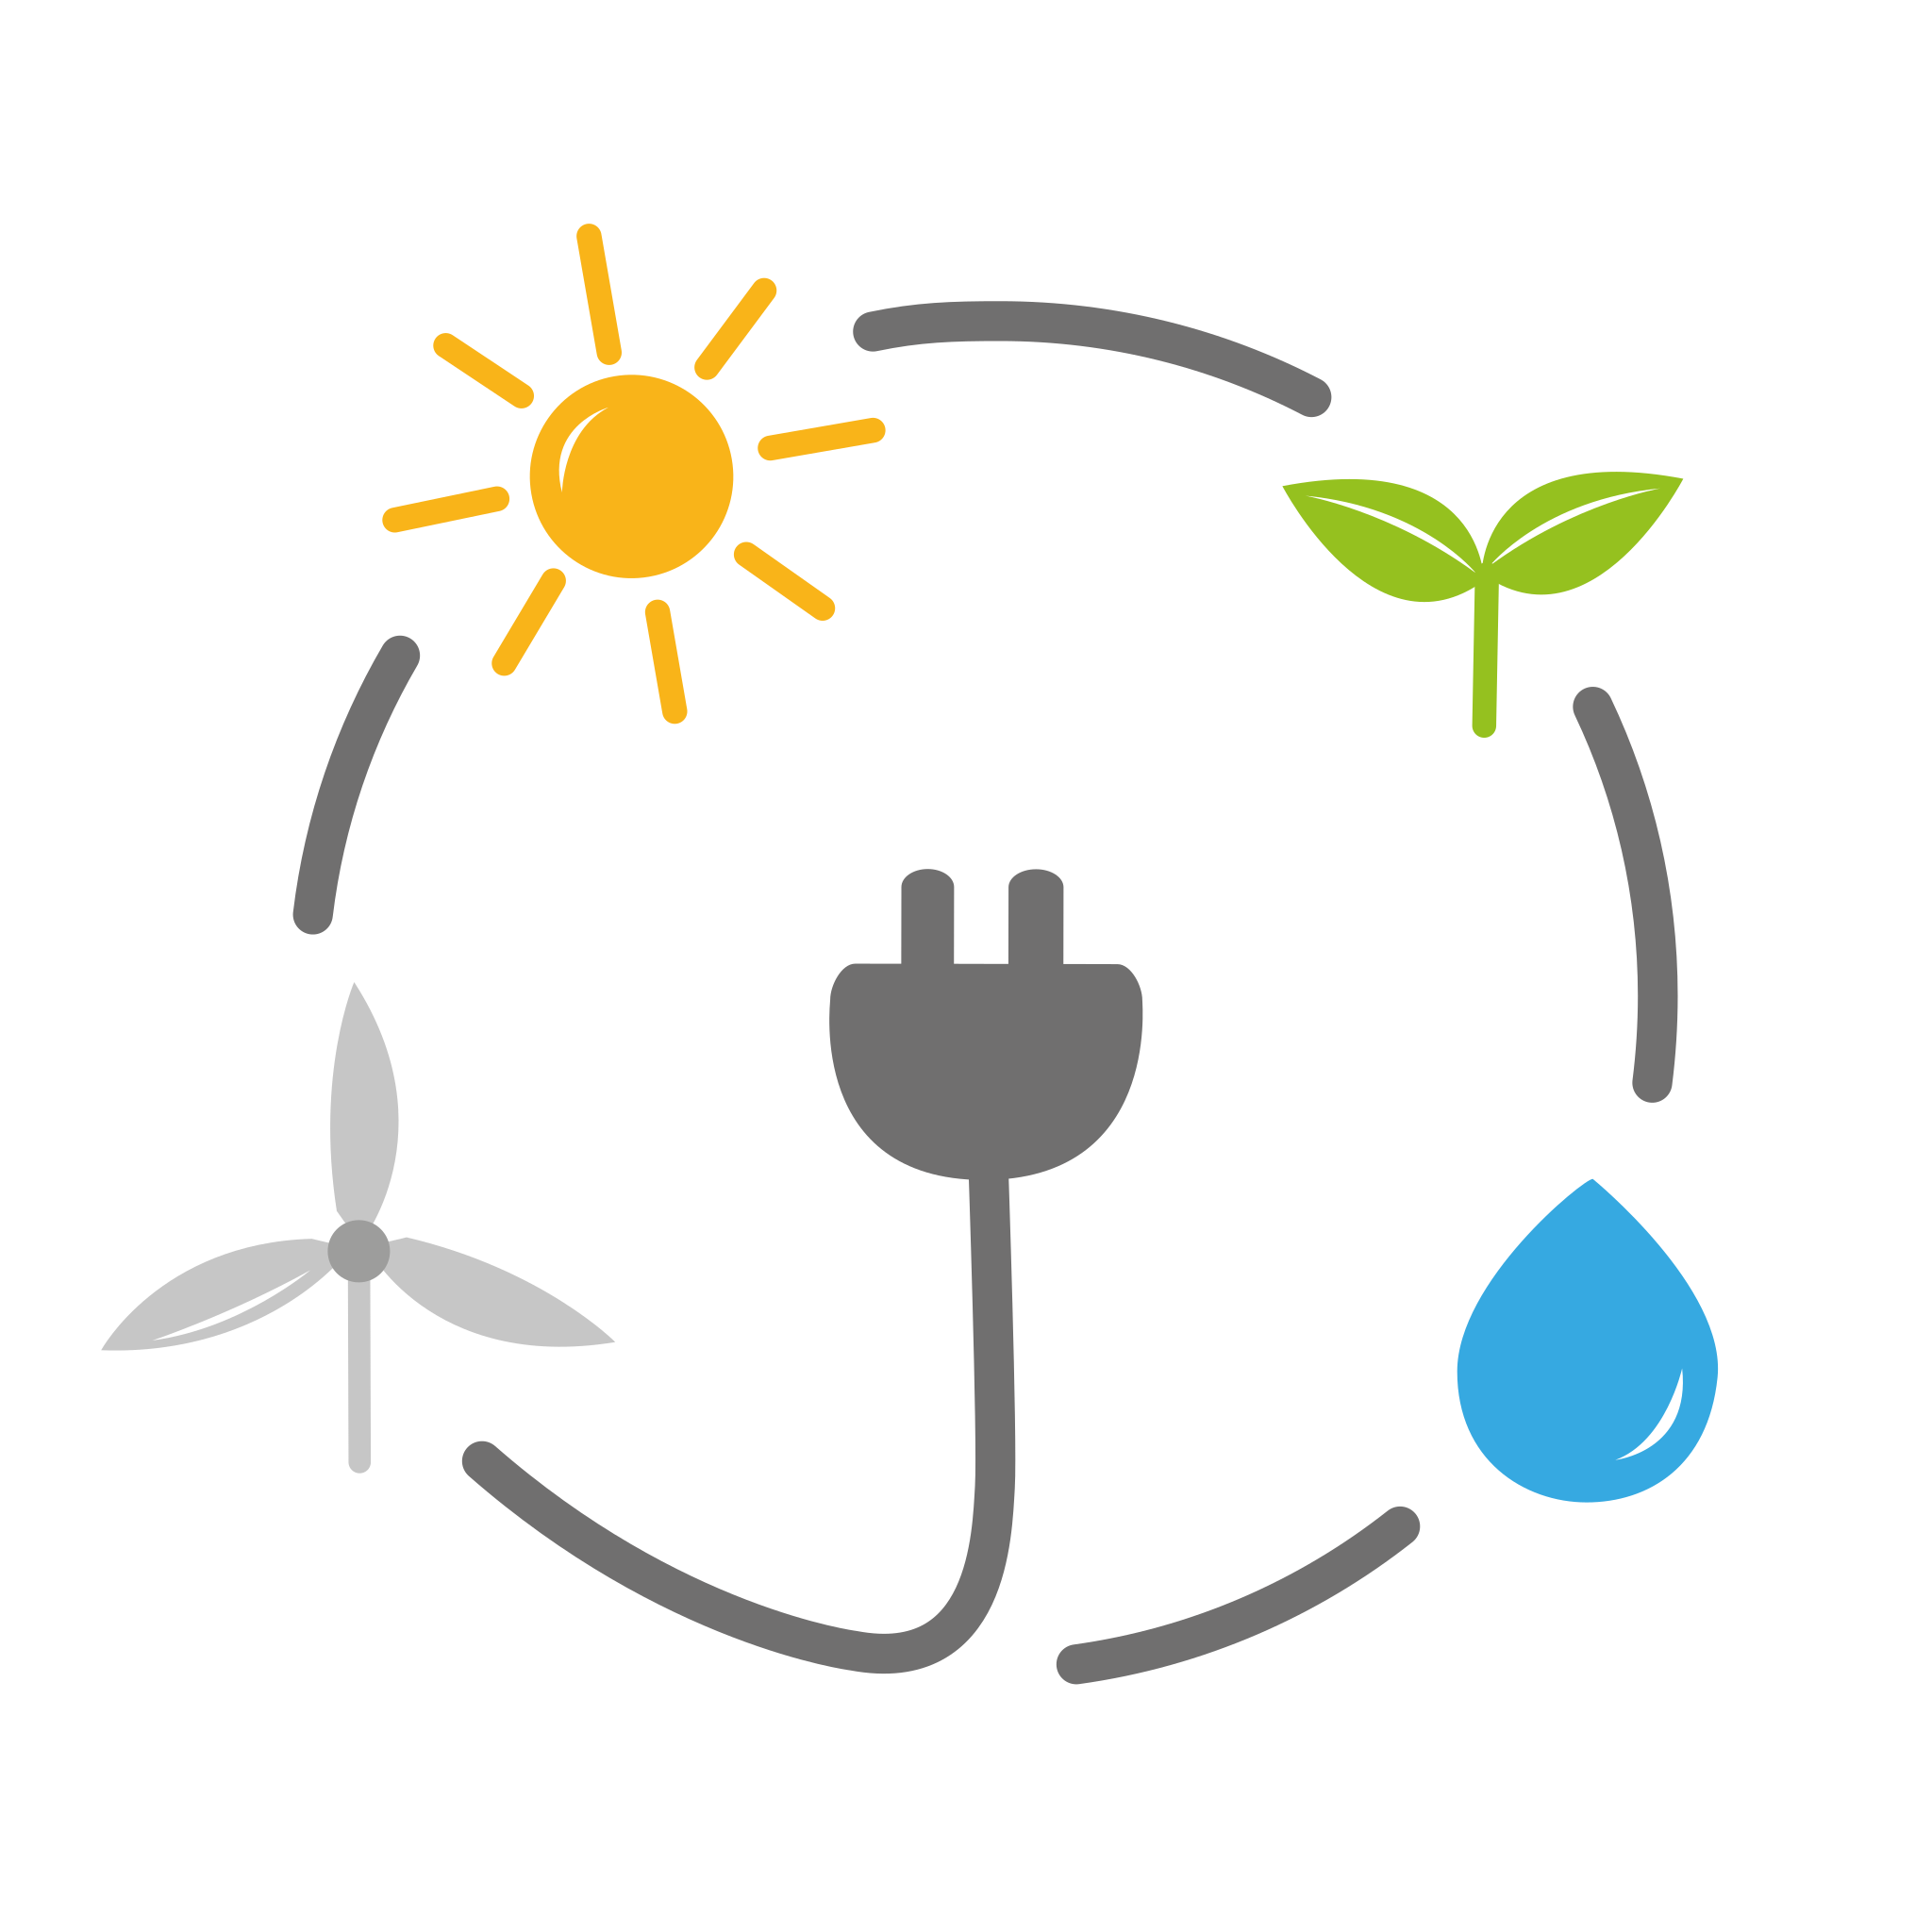
\includegraphics[width=0.8\textwidth]{pictures/renew-book-cover-art}
  \end{center}
  \vfill
  \noindent
  \color{black}
  \raggedleft{\Huge\textbf{พลังงานหมุนเวียนในประเทศไทย}}
  \vskip\baselineskip
  \noindent
  {\huge\color{Black}{สัปปินันทน์ เอกอำพน}}
\end{titlepage}

\restoregeometry
\pagecolor{White}

\frontmatter


\chapter{คำนำ}
\label{sec:org8dc3a72}

ตำราเล่มนี้ถูกเขียนขึ้นเพื่อใช้ประกอบการเรียนการสอนเกี่ยวกับการใช้พลังงานแสงอาทิตย์สำหรับนักศึกษาปี ๓ - ๔ และสำหรับบุคคลทั่วไปที่มีความสนใจทางด้านดังกล่าว โดยที่แม้เนื้อหาบางส่วนจะมีคณิตศาสตร์ชั้นสูงเพื่อช่วยในการแสดงความสัมพันธ์ระหว่างตัวแปร แต่ความตั้งใจหลักของผู้เขียนต้องการจะให้ผู้ที่มีความสนใจและมีพื้นฐานคณิตศาสตร์ระดับมัธยมปลายควรจะสามารถอ่านแล้วเข้าใจได้ ทั้งนี้เนื่องจากผู้เขียนเล็งเห็นความสำคัญของการสร้างความเข้าใจพื้นฐานเรื่องของพลังงานแสงอาทิตย์ รวมถึงเทคโนโลยีต่างๆที่จะนำไประยุกต์ใช้เพื่อกักเก็บ แปลง หรือนำพลังงานนี้ไปใช้ เพื่อให้ผู้อ่านจะได้มีความเข้าใจที่ถูกต้อง มีพื้นฐานความรู้ที่เหมาะสมในการทำงานในเทคโนโลยีพลังงานสะอาดในอนาคต หรือแม้แต่สามารถทำความเข้าใจและคำนึงถึงความเหมาะสมของนโยบายหรือโครงการที่เกี่ยวกับพลังงานแสงอาทิตย์ได้โดยไม่เชื่อเพียงคำโฆษณาหรืออวดอ้างที่อาจจะเกินความเป็นจริง

ผู้เขียนหวังว่าข้อมูลที่ได้รับการรวบรวมไว้ในตำราเล่มนี้จะเป็นประโยชน์ต่อผู้อ่านในวงกว้าง มิใช่เฉพาะระดับนักศึกษาหรือนักวิชาการเท่านั้น อย่างไรก็ดี ถ้าหากผู้อ่านมีความรู้พื้นฐานทางด้านฟิสิกส์พื้นฐาน จะทำให้สามารถเข้าใจเนื้อหาและบทวิเคราะห์ได้ดียิ่งขึ้น รวมถึงสามารถนำความรู้ที่ได้รับนำไปวิเคราะห์ข้อมูลอื่นๆได้ด้วยตนเอง

สัปปินันทน์ เอกอำพน

\tableofcontents

\listoffigures

\listoftables

\mainmatter

\chapter{พลังงานแสงอาทิตย์}
\label{sec:org65a1b3a}

\epigraph{ผมพนันไว้เลยว่าพระอาทิตย์และพลังงานแสงอาทิตย์จะต้องมาแน่ๆ พลังงานมันมากมายมหาศาลเหลือเกิน หวังว่าเราคงจะไม่ต้องรอจนกว่าน้ำมันกับถ่านหินจะหมดก่อนถึงจะได้ใช้นะ I'd put my money on the sun and solar energy. What a source of power! I hope we don't have to wait until oil and coal run out before we tackle that.}{Thomas A. Edison}

เวลาพูดถึงพลังงานแสงอาทิตย์นั้น
หลายๆคนอาจจะนึกถึงแดดร้อนๆในช่วงเดือนมีนาคมหรือเมษายน
แต่จริงๆแล้วจะรู้ไหมว่าพลังงานที่มีอยู่ในแสงอาทิตย์นั้นประกอบด้วยหลายส่วน
การจะตักตวงพลังงานแสงอาทิตย์มาใช้ให้ได้เต็มที่นั้น
จำเป็นที่เราจะต้องมีความเข้าใจถึงส่วนประกอบเหล่านี้

เนื่องจากพลังงานแสงอาทิตย์นั้นเป็นพลังงานที่เกิดขึ้นมาจากการแผ่รังสีของดวงอาทิตย์ออกมาในรูปของคลื่นแม่เหล็กไฟฟ้าในช่วงคลื่นต่างๆ
ดังนั้นเราควรจะเริ่มทำความเข้าใจกับการแผ่รังสีของวัตถุดำก่อน

\section{การแผ่รังสีของวัตถุดำ}
\label{sec:org23e7eab}

การแผ่รังสีของวัตถุดำ (blackbody radiation) เกิดจากการแผ่รังสีคลื่นแม่เหล็กไฟฟ้าจากความร้อนของวัตถุซึ่งอยู่ในสภาวะสมดุลทางอุณหพลศาสตร์กับสิ่งแวดล้อม ซึ่งช่วงความถี่และความเข้มข้นของคลื่นต่างๆนั้นขึ้นอยู่กับอุณหภูมิของวัตถุดังกล่าว อย่างไรก็ดี ในความเป็นจริงแล้วไม่มีวัตถุได้ที่มีการแผ่รังสีเหมือนวัตถุดำแท้จริง โดนเฉพาะอย่างยิ่งดาวฤกษ์อย่างพระอาทิตย์นั้นก็ไม่ได้อยู่ในสภาวะสมดุลกับสิ่งแวดล้อม แต่ความเข้าใจเรื่องของการแผ่รังสีนี้ก็สามารถนำมาใช้ทำความเข้าใจส่วนประกอบของแสงอาทิตย์ได้

ยกตัวอย่างเช่น ในวัตถุที่มีอุณหภูมิต่ำนั้น ในห้องมืดจะมองเห็นเป็นสีดำเนื่องจากช่วงคลื่นที่แผ่ออกมาเป็นช่วงอินฟราเรดซึ่งมองด้วยตาเปล่าไม่เห็น เมื่ออุณหภูมิสูงขึ้นถึงราว 500\(^{\circ}\) C การแผ่รังสีเริ่มเข้าอยู่ในช่วงความถี่ที่ตามองเห็น (visible spectrum) และจะเริ่มมีสีแดง เมื่ออุณหภูมิสูงมากจะออกเป็นสีฟ้าขาว เมื่อวัตถุมีการแผ่รังสีเป็นสีขาว แสดงว่ามีการแผ่รังสีบางส่วนออกมาเป็นรังสีอัลตราไวโอเลต

ดวงอาทิตย์ซึ่งมีอุณหภูมิที่ผิวประมาณ 5800 K นั้น มีการแผ่รังสีออกมามากที่สุดในช่วงคลื่นแสงและอินฟราเรด และมีจำนวนอีกเล็กน้อยในช่วงอัลตราไวโอเลต

\section{ทิศทางของแสงอาทิตย์}
\label{sec:org3ee4b91}
เนื่องจากดวงอาทิตย์เคลื่อนที่อยู่ตลอดเวลา และพลังงานของแสงอาทิตย์ที่ตกกระทบลงบนพื้นที่หนึ่งๆขึ้นอยู่กับความเข้มข้นของแสงและมุมตกกระทบ เพื่อจะเพิ่มพลังงานแสงอาทิตย์ที่ได้รับ เราสามารถออกแบบอุปกรณ์ให้มีความสามารถในการติดตามดวงอาทิตย์ (solar tracking) ซึ่งในปัจจุบันมีเทคโนโลยีหลายวิธีที่ใช้ในการติดตาม ซึ่งแบ่งได้เป็น 2 ประเภทใหญ่

\section{การติดตามแบบใช้พลังงาน}
\label{sec:org7085368}
การติดตามดวงอาทิตย์แบบใช้พลังงานหรือที่เรียกว่า Active Tracking
นั้นเป็นการใช้ระบบ Feedback Loop
โดยใช้ตัวรับแสงเพื่อช่วยในการบอกตำแหน่งของดวงอาทิตย์ที่ประเมินผล
แล้วส่งสัญญาณให้กับระบบควบคุมให้เคลื่อนที่ไปยังตำแหน่งที่ต้องการ

\section{การติดตามแบบไม่ใช้พลังงาน}
\label{sec:org2bded8b}
วิธีการติดตามดวงอาทิตย์แบบไม่ใช้พลังงาน (Passive Tracking)
ใช้ความร้อนจากแสงอาทิตย์ที่ตกกระทบในการสร้างความเปลี่ยนแปลงในกลไกเพื่อจะปรับทิศทางของตัวรับแสง
ซึ่งมีตัวอย่างดังนี้

\begin{enumerate}
\item แผ่นโลหะประกอบ

ระบบติดตามแสงอาทิตย์โดย \ldots{} ทำมาจากน้ำหนักที่ประกอบเข้ากับแผ่นโลหะ 2 ชนิดซึ่งมีสัมประสิทธิ์การขยายตัวจากความร้อนต่างกัน เมื่อแผ่นโลหะประกอบได้รับความร้อนจากแสงอาทิตย์ โลหะทั้งสองชนิดจะขยายตัวไม่เท่ากันทำให้เกิดการโค้งงอของแผ่น ซึ่งสามารถนำไปใช้ในการปรับถ่วงน้ำหนักตัวรับแสงได้

\item ท่อบรรจุของเหลว-แก็ส

ระบบติดตามด้วยหลักการนี้ใช้ของเหลวที่มีจุดเดือดต่ำบรรจุในท่อสองด้านของตัวรับแสง
ด้านที่ได้รับแสงจะเกิดความร้อน
ทำให้ของเหลวที่อยู่ด้านในเปลี่ยนสถานะเป็นแก๊ส
ผลักดันให้ของไหลที่เหลือไปอยู่ที่ด้านที่ไม่โดนแสง
ทำให้เกิดความไม่สมดุลของน้ำหนักของตัวรับแสง
ซึ่งจะปรับทิศทางตามความไม่สมดุลที่เกิดขึ้นโดยหันเข้าหาทิศทางของดวงอาทิตย์
\end{enumerate}

\section{วิถีการติดตามแสงอาทิตย์}
\label{sec:orge254580}
กลไกในการติดตามแสงอาทิตย์ทำได้ไดยการควบคุมมุนของแผงติดตาม
ซึ่งมุมที่อยู่ควบคุมนี้จะเป็นมุมที่ตั้งฉากกันเพื่อให้การควบคุมแต่ละมุมเป็นอิสระต่อกัน
โดยวิถีการติดตามมีสองแบบดังนี้

\begin{enumerate}
\item Clock-declination โดยมุมที่ใช้ในการควบคุมคือมุมตามทิศตะวันออก-ตะวันตก
(\(\theta_{CL}\)) และมุมเงย (\(\theta_{DE}\))

\item Pseudo-azimuthal ควบคุมโดยใช้มุมอซิมุทและมุมเงย
\end{enumerate}

\chapter{เซลล์แสงอาทิตย์}
\label{sec:orgb157a80}

เซลล์แสงอาทิตย์ (Solar cell หรือ Photovoltaic cell)
เป็นอุปกรณ์ที่สามารถแปลงพลังงานจากคลื่นแม่เหล็กไฟฟ้าในแสงอาทิตย์ให้เป็นพลังงานไฟฟ้าได้โดยตรงโดยใช้ปรากฏการณ์โฟโตโวลตาอิก
(Photovoltaic effect)
ปรากฏการณ์นี้เกิดขึ้นจากการเคลื่อนไหวของอิเลกตรอนในเซลล์แสงอาทิตย์เมื่อได้ดูดซับพลังงานแสงอาทิตย์
ซึ่งทำให้เกิดกระแสไฟฟ้าซึ่งสามารถนำไปใช้ให้เกิดประโยชน์ได้

จริงๆแล้วปรากฏการณ์โฟโตโวลตาอิกนั้นสามารถเกิดขึ้นได้ในวัสดุอื่นๆนอกจากเซลล์สุริยะด้วย
แต่เนื่องจากการเคลื่อนที่ของอิเลกตรอนจากปรากฏการณ์ดังกล่าวนั้นไม่มีทิศทางหรือแนวโน้มใดๆ
จึงทำให้ไม่มีกระแสลัพธ์เกิดขึ้น
จำเป็นจะต้องมีวิธีบังคับการไหลของอิเลกตรอนเพื่อให้เกิดกระแสได้
นั่นเป็นสาเหตุที่เซลล์สุริยะจำเป็นจะต้องมีการออกแบบวงจรพิเศษ

\section{หลักการทำงานของเซลล์แสงอาทิตย์}
\label{sec:orgae7bd3f}
ในเซลล์สุริยะนั้น
ระบบวงจรที่จะบังคับทิศทางการไหลของอิเลกตรอนที่เกิดจากปรากฏการณ์โฟโตโวทาอิกคือ
P-N junction ซึ่งเป็นการเชื่อมต่อระหว่างสารกึ่งตัวนำประเภทบวก (P-type)
กับประเภทลบ (N-type) โดยที่สาร P-type นั้นมีหลุมอิเลกตรอนเนื่องมาจากการ
dope สารที่ขาดอิเลกตรอนลงไปในซิลิกอน ส่วนสาร N-type
นั้นมีอิเลกตรอนอิสระเนื่องจากการ dope สารที่มีอิเลกตรอนอิสระลงไป
เมื่อนำสารทั้งสองแบบมาเชื่อมต่อกัน
หลุมอิเลกตรอนและอิเลกตรอนอิสระเคลื่อนที่เข้าหากันทำให้เกิด \textbf{Depletion
Zone} ซึ่งป้องกันการไหลของอิเลกตรอนอีก เมื่อแสงอาทิตย์ตกกระทบ
อิเลกตรอนอิสระและหลุมอิเลกตรอนที่เกิดขึ้นจึงถูกบังคับให้ไหลผ่านความต้านทานภายนอกซึ่งทำให้เกิดกระแสไฟฟ้าขึ้น

ปริมาณกระแสที่เซลล์แสงอาทิตย์สร้างขึ้นได้นั้นขึ้นอยู่กับปัจจัยหลายประการ
เช่น ประสิทธิภาพของ P-N junction ในการป้องกันกระแสย้อนกลับ
และประสิทธิภาพของวัสดุเซลล์ในการสร้างอิเลกตรอนเมื่อมีแสงอาทิตย์ตกกระทบ
ซึ่งระบบเซลล์แสงอาทิตย์สามารถเขียนแทนได้ด้วยวงจรเทียบเท่าได้โดยไดโอดและความต้านทานภายในดังรูปที่ \ref{orgcec09ab}


\begin{figure}[h]
  \centering
  \ctikzset{bipoles/length=1cm}
  \begin{tikzpicture}
    \draw[color=Black] (0,0) to [I,l^=$i_{PV}$] ++(90:3) to [short] ++(0:1) to [Do, i=$i_D$] ++(-90:3) to [short] ++(180:1);
    % \draw[color=Black] (1,3) to [short] ++(0:1) to [R,l^=$R_{SH}$,i=$I_{SH}$] ++(-90:3) to [short] ++(180:1);
    \draw[color=Black] (1,3) to [R,l^=$R_s$, i=$i$, -*] ++(0:3);
    \draw[color=Black] (1,0) to [short,-*] ++(0:3);
    \node at (4,1.5) {$V_L$};
  \end{tikzpicture}
\caption{\label{orgcec09ab}วงจรเทียบเท่าของเซลล์แสงอาทิตย์}
\end{figure}

จากวงจรเทียบเท่าดังกล่าว
สามารถเขียนสมการแสดงปริมาณกระแสที่เซลล์สุริยะได้ว่า
กระแสที่ไหลผ่านไปที่โหลดภายนอกเท่ากับกระแสที่เซลล์สุริยะสร้างได้ลบด้วยกระแสที่ไหลย้อนผ่าน
P-N junction

\begin{equation}
\label{eq:org4975087}
  i = i_{PV} - i_D
\end{equation}

ปริมาณกระแสที่ไหลผ่าน P-N junction ขึ้นอยู่กับอุณหภูมิ (\(T\))
และความต่างศักย์ของโหลดภายนอก (\(V\)) โดยสามารถเขียนเป็นสมการได้ดังนี้

\begin{equation}
\label{eq:orgb1c36fe}
  i_D = i_0 \left[ exp \left( \frac{eV}{kT} \right) - 1 \right]
\end{equation}

เมื่อแทนสมการ \ref{eq:orgb1c36fe} ลงในสมการ
\ref{eq:org4975087} จะได้สมการ

\begin{equation}
\label{eq:org6b60a1a}
  i = i_{PV} - i_0\left[exp \left( \frac{eV}{kT} \right) - 1 \right]
\end{equation}

โดยที่ \(i_0\) คือกระแสย้อนกลับอิ่มตัวของ P-N junction, \(i_{PV}\)
คือกระแสจากปรากฏการณ์โฟโตโวลทาอิก และ \(i\)
คือกระแสที่ผ่านตัวต้านทานภายนอก

เซลล์สุริยะสามารถผลิตกำลังได้สูงสุดเมื่อ

\begin{align}
\label{eq:orge1e26dd}
  P_{out} &= i V \nonumber \\
  \frac{dP_{out}}{dV} &= 0 \nonumber \\
  exp \left(\frac{e V_{\max P}}{kT} \right) &= \dfrac{1+\dfrac{i_{PV}}{i_0}}{1+ \dfrac{e V_{\max P}}{kT}}
\end{align}

สังเกตว่าสมการนี้มีค่า \(V_{\max P}\) อยู่ทั้งสองด้าน
ไม่สามารถแก้สมการเชิงวิเคราะห์ได้ จำเป็นต้องแก้สมการเชิงตัวเลข

ประสิทธิภาพสูงสุดของแผงเซลล์สุริยะเกิดในตอนที่แผงผลิตกำลังไฟฟ้าสูงสุด
ซึ่งเขียนเป็นสมการได้ว่า

\begin{gather*}
\label{eq:org8069bb3}
  P_{\max} =  \dfrac{V_{\max P} ( i_0 + i_{PV} )}{1 + \dfrac{kT}{e V_{\max P}}} \\
  \eta_{\max} = \eta_{\max P} =  \dfrac{P_{\max}}{I_{in}} = \dfrac{V_{\max P} ( i_0 + i_{PV} )}{I_{in} \left(1 + \dfrac{kT}{e V_{\max P}} \right)}
\end{gather*}

\begin{figure}[h]
  \centering
  \begin{tikzpicture}
    \begin{axis} [
      scale only axis,
      % xtick=data,
      xmin=0,xmax=0.5,
      ymin=0,ymax=4,
      xtick distance=0.1,
      xlabel={ความต่างศักย์ $V$ [V]},
      ylabel={กระแส $I$ [A]},
      axis y line*=left,
      ]
      \addlegendimage{empty legend}
      \label{plot_0}
      \addplot [blue, domain=0:0.45, samples=50] {3.5 - 10^(-7)*(exp(\x/0.0259)-1)};
      \label{plot_1}
      \addplot [red, domain=0:0.4, samples=50] {3.5 - 10^(-6)*(exp(\x/0.0259)-1)};
      \label{plot_2}
      \addplot [green, domain=0:0.35, samples=50] {3.5 - 10^(-5)*(exp(\x/0.0259)-1)};
      \label{plot_3}
    \end{axis}
    \begin{axis} [
      scale only axis,
      axis y line*=right,
      axis x line=none,
      xmin=0,xmax=0.5,
      ymin=0,ymax=1.5,
      ylabel={กำลังไฟฟ้า [W]},
      compat=1.3,
      ytick distance=0.3,
      legend style={at={(0.1,0.6)}, anchor=west},
      ]
      \addlegendimage{/pgfplots/refstyle=plot_0}\addlegendentry{\hspace{-6mm}\textbf{กระแส}};
      \addlegendimage{/pgfplots/refstyle=plot_1}\addlegendentry{$10^{-7}$}
      \addlegendimage{/pgfplots/refstyle=plot_2}\addlegendentry{$10^{-6}$}
      \addlegendimage{/pgfplots/refstyle=plot_3}\addlegendentry{$10^{-5}$}
      \addlegendimage{empty legend}
      \addplot [blue, dashed, domain=0:0.45] {\x * (3.5 - 10^(-7)*(exp(\x/0.0259)-1))};
      \addplot [red, dashed, domain=0:0.4] {\x * (3.5 - 10^(-6)*(exp(\x/0.0259)-1))};
      \addplot [green, dashed, domain=0:0.35] {\x * (3.5 - 10^(-5)*(exp(\x/0.0259)-1))};
      \addlegendentry{\hspace{-6mm}\textbf{กำลัง}};
      \addlegendentry{$10^{-7}$};
      \addlegendentry{$10^{-6}$};
      \addlegendentry{$10^{-5}$};
    \end{axis}
  \end{tikzpicture}
  \caption{กราฟแสดงความสัมพันธ์ระหว่างกระแส แรงดันไฟฟ้า และกำลังไฟฟ้าที่ผลิตได้จากในเซลล์แสงอาทิตย์ที่อุณหภูมิ 25$^{\circ}$C}
\end{figure}

\subsection{Example}
\label{sec:org85da596}
กำลังและประสิทธิภาพของเซลล์สุริยะ

เซลล์สุริยะหนึ่งมีพื้นที่ 2 m\(^{\text{2}}\)
ในคู่มือระบุว่ามีคุณสมบัติดังนี้

\begin{center}
\begin{tabular}{ll}
\toprule
Properties & Value (A/m\(^{\text{2}}\))\\[0pt]
\midrule
\(i_{pv}\) & \(0.3 I_{rad}\)\\[0pt]
\(i_0\) & \(10^{-8}\)\\[0pt]
\bottomrule
\end{tabular}
\end{center}

บริเวณที่ติดตั้งมีกำลังจากแสงอาทิตย์โดยเฉลี่ย 250 W/m\(^2\)
ระหว่างการทำงาน แผงเซลล์สุริยะจะมีอุณหภูมิ 50 C จงคำนวณหา

\begin{enumerate}
\item กำลังไฟฟ้าสูงสุดที่ผลิตได้

\item ประสิทธิภาพของเซลล์สุริยะนี้
\end{enumerate}

\subsection{Solution}
\label{sec:org5739fd1}
จากสมการ \ref{eq:orge1e26dd} เราจะสามารถคำนวณหาค่าความต่างศักย์ที่สร้างกระแสไฟฟ้าสูงสุด
\(P_{\max P}\) ได้ดังนี้

\begin{align*}
  \exp \left(\frac{e V_{\max P}}{kT} \right) &= \dfrac{1+\dfrac{i_{PV}}{i_0}}{1+ \dfrac{e V_{\max P}}{kT}} \\
  \exp \left(\frac{ 1.6 \times 10^{-19} V_{\max P} }{ 1.38 \times 10^{-23} \times (50 + 273)} \right) &= \dfrac{1+ \dfrac{0.3 \times 250}{10^{-8}}}{1+\dfrac{1.6 \times 10^{-19} V_{\max P}}{1.38 \times 10^{-23} \times (50 + 273)}} \\
  V_{\max} &= 0.549 \text{ V}
\end{align*}

เมื่อคำนวณ \(V_{\max P}\)
ได้แล้วเราจะสามารถคำนวณหากำลังไฟฟ้าสูงสุดที่จะสามารถสร้างได้เท่ากับ

\begin{align*}
    P_{\max} &=  \dfrac{V_{\max P} ( i_0 + i_{PV} )}{1 + \dfrac{kT}{e V_{\max P}}} \\
             &= \dfrac{0.549 \left(10^{-8} + 75\right)}{1 + \dfrac{ 1.38 \times 10^{-23} (50 + 273)}{1.6 \times 10^{-19} (0.549)}} \\
             P_{\max} &= 39.189 \text{ W}
  \end{align*}

ประสิทธิภาพของแผงเซลล์แสงอาทิตย์สามารถคำนวณได้จากกำลังไฟฟ้าที่ผลิตได้หารด้วยกำลังของรังสีแสงอาทิตย์ที่ตกกระทบบนแผง

\begin{align*}
  \eta &= \frac{P_{\max}}{I_{rad}} \\
       &= \frac{39.189}{250} \\
&= 0.157
\end{align*}

\chapter{พลังงานความร้อนแสงอาทิตย์}
\label{sec:org05a8cb3}
พลังงานความร้อนจากแสงอาทิตย์ได้รับการนำมาใช้ตั้งแต่โบราณกาลในชีวิตประจำวันไม่ว่าจะเป็นการถนอมอาหาร
การตากแห้ง หรือเพื่อกับเก็บไว้ใช้ในภายหลัง ในบทนี้
เราจะมาพิจารณาการเพิ่มประสิทธิภาพการสร้างพลังงานความร้อนและการนำพลังงานนั้นมาใช้

\section{Solar Collectors}
\label{sec:org68d1863}

\begin{itemize}
\item Heat exchangers collecting solar radiation \(\rightarrow\) heat transported by fluid
\end{itemize}

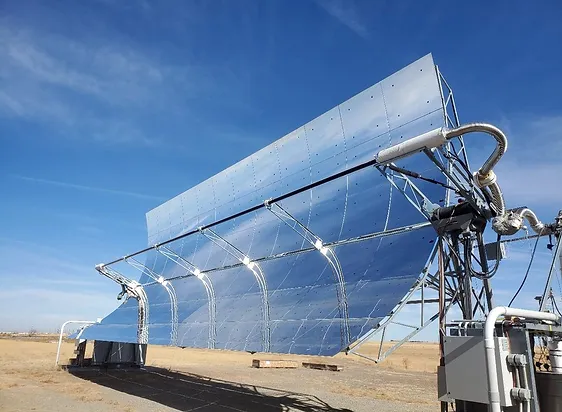
\includegraphics[height=0.45\textheight]{./pictures/parabolic-collector.png} 
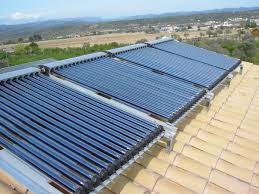
\includegraphics[height=0.45\textheight]{./pictures/flat-plate-collector.jpg} 

\section{วัสดุรับแสงอาทิตย์}
\label{sec:orgebe1b7f}

\begin{itemize}
\item Use to allow solar radiation through (short-wave radiation)
\item Prevent heat loss through convection and long-wave radiation
\item Glasses (low long-wave transmission) is best, plastics are ok (medium long-wave transmission)
\end{itemize}


\subsection{วัสดุที่เหมาะสม}
\label{sec:orga91c853}

\begin{itemize}
\item absorb solar radiation (high absorbance \(\alpha\))
\item convert to heat
\item transfer to working fluid with min loss (low emittance \(\varepsilon\))
\item "selective surface"
\end{itemize}

\subsection{Selective Surfaces}
\label{sec:org6458694}

\begin{itemize}
\item Thin high \(\alpha\) with high transmission to shortwave
\item bottom layer is highly reflective and low \(\varepsilon\) to longwave
\item Crucial for collector whose \(T \gg T_{a}\)

\begin{itemize}
\item Black chrome
\end{itemize}

\begin{center}
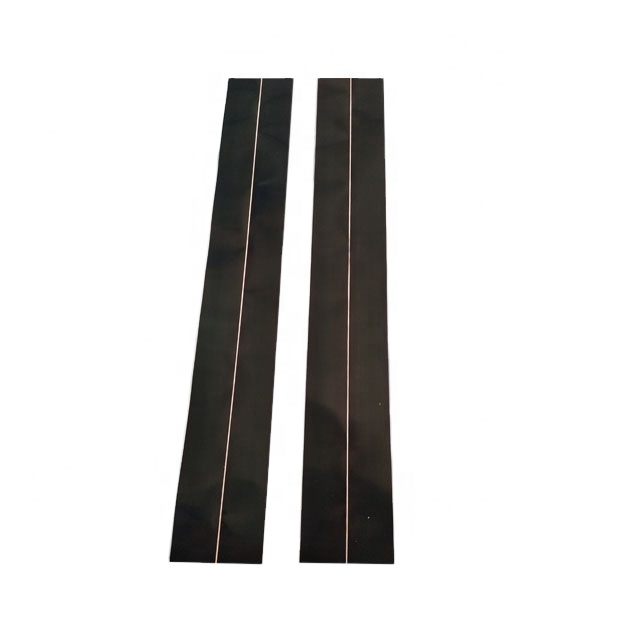
\includegraphics[height=0.4\textheight]{./pictures/black-chrome.jpg}
\end{center}
\end{itemize}


\begin{center}

\includegraphics[height=0.4\textheight]{./pictures/black-anodized-alum.jpg}
\end{center}


\section{ชนิดของ Solar Collector}
\label{sec:orgf04ef72}

\begin{itemize}
\item แผ่นรับแสงอาทิตย์แบบแบน (flat-plate solar collector)
\item แผ่นรับแสงอาทิตย์แบบรวมแสง (concentrating solar collector)
\end{itemize}

\section{แผ่นรับแสงอาทิตย์แบบแบน}
\label{sec:org488cf76}

ส่วนประกอบของแผ่นรับแสงอาทิตย์แบบแบน

\begin{center}
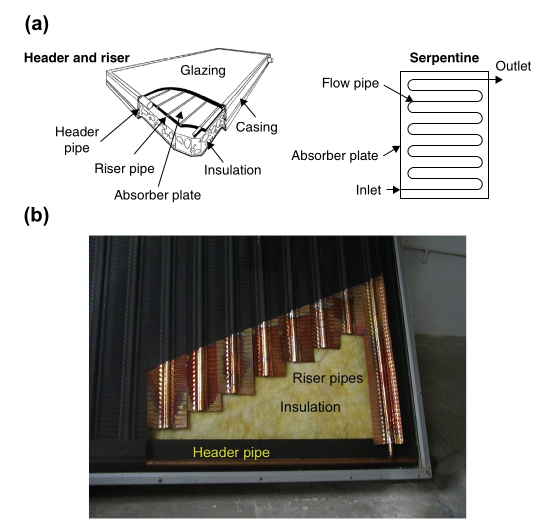
\includegraphics[height=0.9\textheight]{./pictures/flat-collector-views.png}
\end{center}


\begin{center}
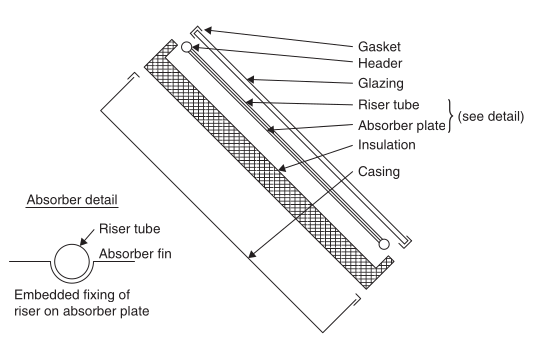
\includegraphics[width=.9\linewidth]{./pictures/flat-collector-components.png}
\end{center}


\begin{itemize}
\item Water systems

\begin{center}
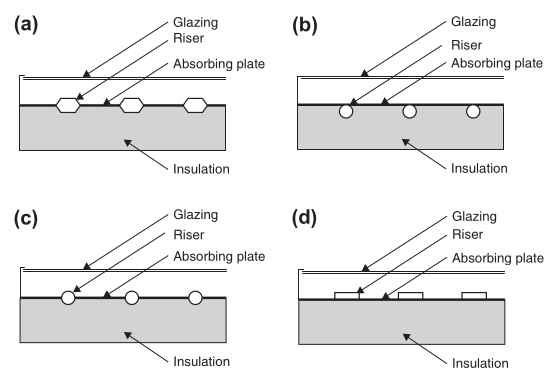
\includegraphics[width=.9\linewidth]{./pictures/water-system.png}
\end{center}
\end{itemize}


\begin{itemize}
\item Air systems

\begin{center}
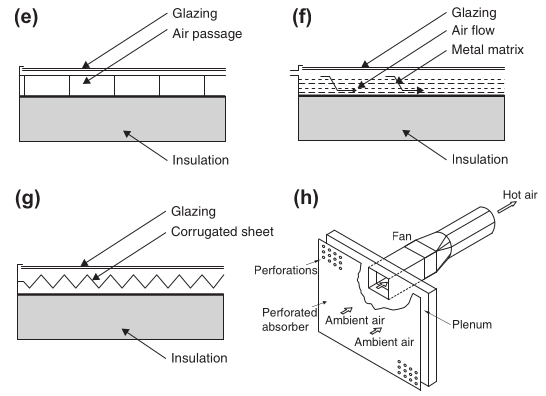
\includegraphics[width=.9\linewidth]{./pictures/air-system.png}
\end{center}
\end{itemize}

\subsection{คำถามคิดสนุก}
\label{sec:orga79118e}

\begin{itemize}
\item What are the main design difference(s) between air and water systems?
\item Why?
\end{itemize}

\section{การวิเคราะห์ความร้อน}
\label{sec:org66448bb}
From \(q_{loss} = U\Delta T\)

\begin{center}
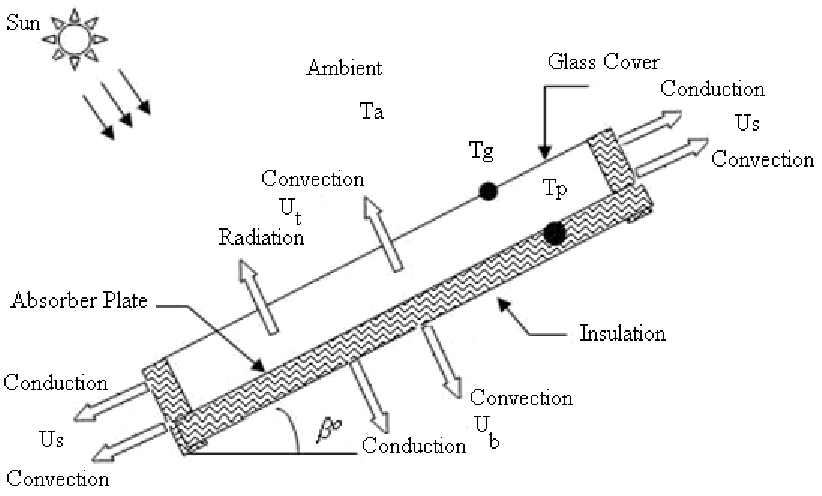
\includegraphics[width=\textwidth]{./pictures/flat-plate-heat-loss.png}
\end{center}

\begin{itemize}
\item Top (\(U_t\))
\item Bottom (\(U_b\))
\item Sides (\(U_e\))

\item Assume steady-state operation
\end{itemize}

การถ่ายเทความร้อนทั้งหมดที่เกิดขึ้นในระบบสามารถอธิบายโดยใช้วงจรความร้อนได้ดังนี้

\begin{figure}[h]
  \centering
  \begin{tikzpicture}
    \draw (0,0) node[above right]{$T_p$} --++ (135:1) to [/tikz/circuitikz/bipoles/length=0.75cm,R=$1/h_{c,p-c}$] ++ (90:1) --++ (45:1);
    \draw (0,0) --++ (45:1) to [/tikz/circuitikz/bipoles/length=0.75cm,resistor,l_=$1/h_{r,p-c}$] ++ (90:1) --++ (135:1) node(Tc){} node[right]{$T_c$};
    \draw (Tc.center) --++ (135:1) to [/tikz/circuitikz/bipoles/length=0.75cm,R=$1/h_{c,c-a}$] ++ (90:1) --++ (45:1);
    \draw (Tc.center) --++ (45:1) to [/tikz/circuitikz/bipoles/length=0.75cm,resistor,l_=$1/h_{r,c-a}$] ++ (90:1) --++ (135:1) node[right]{$T_a$};
    \draw (0,0) --++ (-135:1) to [/tikz/circuitikz/bipoles/length=0.75cm,resistor,l_=$1/h_{c,b-a}$] ++ (-90:1) --++ (-45:1);
    \draw (0,0) --++ (-45:1) to [/tikz/circuitikz/bipoles/length=0.75cm,R=$1/h_{r,b-a}$] ++ (-90:1) --++ (-135:1) node[right]{$T_a$};
    \draw [stealth-, thick] (0,0) ++ (180:0.1) --++ (180:2) node[left]{$S$};
    \draw [-stealth, thick] (0,0) ++ (0:0.1) --++ (0:2) node[right]{$Q_{u}$};
  \end{tikzpicture}
\end{figure}

การสูญเสียความร้อนไปที่ด้านบนของเครื่องมีเกิดจากกระบวนการนำและพาความร้อน ซึ่งสามารถเขียนเป็นสมการได้ว่า

\begin{align*}
  q_{loss} &= h_{c,p-c1}(T_{p} - T_{c1}) + \frac{\sigma(T_{p}^{4} - T_{c1}^{4})}{\dfrac{1}{\varepsilon_{p}} + \dfrac{1}{\varepsilon_{c1}} - 1} \\
	   &= (h_{c,p_{c1}} + h_{r,p-c1})(T_{p}- T_{c1})
\end{align*}

โดยที่
\begin{align*}
  h_{r,p-c} &= \frac{\sigma(T_{p}+T_{c})(T_{p}^{2} + T_{c}^{2})}{\frac{1}{\varepsilon_{p}} + \frac{1}{\varepsilon_{c}} - 1}
\end{align*}

ความต้านทานต่อการสูญเสียความร้อน \(R_1\) เท่ากับ
\begin{align*}
  R_{1} &= \frac{1}{h_{c,p-c} + h_{r,p-c}}
\end{align*}

การสูญเสียความร้อนจากแผ่นครอบ (cover) ไปถึงสภาพแวดล้อมเกิดได้จากการพาความร้อนของลม และการแผ่รังสีไปสูสภาพแวดล้อม
\begin{align*}
  q_{loss} &= h_w(T_{c} - T_{a}) + \sigma\varepsilon_c(T_{c}^{4} - T_{s}^{4}) \\
  	 &= (h_{w} + h_{r,c-a})(T_{c}- T_{a})
\end{align*}

โดยที่ค่าสัมประสิทธิ์การแผ่รังสีไปสู่สภาพแวดล้อมคือ
\begin{align*}
  h_{r,c-a} &= \frac{\sigma\varepsilon_c(T_c^4 - T_s^4)}{T_c - T_a}
\end{align*}

ดังนั้น ความต้านทานต่อการสูญเสียความร้อนจากแผ่นครอบไปจนถึงสภาพแวดล้อมสามารถคำนวณได้จาก
\begin{align*}
  R_{2} &= \frac{1}{h_{w} + h_{r,c-a}}
\end{align*}

เมื่อพิจารณาจากวงจรความร้อน จะเห็นได้ว่าความต้านทานทั้งสองต่อกันแบบอนุกรม เราจึงสามารถคำนวณความต้านทานรวมได้ว่า
\begin{align*}
  R_{t} &= R_{1} + R_{2}
\end{align*}

และสามารถคำนวณสัมประสิทธิ์การสูญเสียความร้อนได้ดังนี้
\begin{align*}
  U_{t} &= \frac{1}{R_{t}} = \left( \frac{1}{h_{c,p-c} + h_{r,p-c}} + \frac{1}{h_{w} + h_{r,c-a}} \right)^{-1}
\end{align*}

การแก้สมการในกรณีนี้อาจมีความซับซ้อนเนื่องจากคุณสมบัติส่วนมากขึ้นกับอุณหภูมิ \(T_c\) ดังนั้น วิธีการหาคำตอบจะต้องใช้การหาคำตอบเชิงตัวเลขโดยการสมมติค่า \(T_c\) เบื้องต้น แก้สมการเพื่อหาค่า \(T_c\) จริงจนกว่าค่าจะลู่เข้าหาคำตอบจริงเพียงพอ (แก้โดยใช้เครื่องคิดเลขอาจจะยาก แต่แก้โดยใช้ spreadsheet หรือโปรแกรมทางคณิตศาสตร์ทำได้สะดวกกว่ามาก)


\subsubsection{Example: Loss Coefficient of a Flat-plate Collector}
\label{sec:org1a3688b}

Calculate loss coefficient for an absorber with a single glass cover having the following specs

\begin{center}
\begin{tabular}{lrl}
Plate-to-cover spacing & 25 & mm\\[0pt]
Plate emissivity & 0.95 & \\[0pt]
Ambient and sky temp & 10 & C\\[0pt]
Wind heat transfer coeff & 10 & W/m\textsuperscript{2}K\\[0pt]
Plate temperature & 100 & C\\[0pt]
Collector tilt & 45 & \\[0pt]
Glass emissivity & 0.88 & \\[0pt]
\end{tabular}
\end{center}

\subsubsection{Solution:}
\label{sec:org568eb51}

Estimate cover temperature so we can calculate \(h_{c,p-c}, h_{r,p-c}, h_{r,c-a}\)

Assume cover temperature of 35 C
The radiative coefficients can be calculated as

\begin{align*}
  h_{r,p-c} &= \frac{\sigma (T_{p}^{2} + T_{c}^{2})(T_{p} + T_{c})}{\frac{1}{\varepsilon_{p}} + \frac{1}{\varepsilon_{c}} - 1} \\
            &= \frac{5.67 \times 10^{-8}(373^{2} + 308^{2})(373 + 308)}{\frac{1}{0.95} + \frac{1}{0.88} - 1} \\
            &= 7.6 \text{ W/m}^2\text{K} \\
  h_{r,c-a} &= \varepsilon_{c}\sigma (T_{c}^{2} + T_{s}^{2})(T_{c} + T_{s}) \\
            &= 0.88(5.67 \times 10^{-8})(308^{2} + 283^{2})(308 + 283) \\
            &= 5.16 \text{ W/m}^2\text{K}
\end{align*}

For convective coefficient, assume average air temp between plate and cover is (100 + 35)/2 = 67.5 C = 340.5 K, at that temp, \(\nu\) = 1.96 \(\times 10^{-5}\) m\(^2\text{/K}\), \(k\) = 0.0293 W/mK, Pr = 0.7
\begin{align*}
  \text{Ra} &= \frac{g\beta\Delta T L^{3}Pr}{\nu^{2}} \\
            &= \frac{9.8(1/340.5)(100 - 35)(0.025^{3})(0.7)}{(1.96 \times 10^{-5})^{2}} \\
            &= 5.33 \times 10^{4} \\
  \text{Nu} &= 1 + 1.44\left[1-\frac{1708 (\sin 1.8(45))^{1.6}}{53300\cos 45}\right]\left[ 1 - \frac{1708}{53300\cos 45}\right]^{+} \\
            & \hspace{5mm} + \left[ \left(\frac{53300 \cos 45}{5830} \right)^{1/3} - 1 \right]^{+} \\
            &= 3.19 \\
\end{align*}

Finally, calculate the convective coefficient by
\begin{align*}
  h_{c,p-c} &= \text{Nu}\frac{k}{L} = 3.19\frac{0.0293}{0.025} \\
            &= 3.73 \text{ W/m}^{2}\text{K}
\end{align*}

Top loss coefficient is

\begin{align*}
  U_{t} &= \left( \frac{1}{3.73 + 7.6} + \frac{1}{5.16 + 10.0} \right)^{-1} \\
        &= 6.46 \text{ W/m}^{2}\text{K}
\end{align*}

Heat flow from plate to cover must be the same as from plate to air

The cover temperature, based on \(U_t\), is
\begin{align*}
  \left( h_{c,p-c} + h_{r,p-c} \right)(T_{p} - T_{c}) &= U_{t}(T_{p} - T_{a}) \\
  T_c &= T_p - \frac{U_t(T_p - T_a)}{h_{c,p-c} + h_{r,p-c}} \\
      &= 100 - \frac{6.46 (100 - 10)}{3.73 + 7.6} \\
      &= 48.5 \text{ C}
\end{align*}

Note that this is not very close to original guess of 35 C --> Repeat the loop with \(T_c = 48.5\) C

Recalculating \(h_{c,p-c}, h_{r,p-c}, h_{r,c-a}\)

\(T_c\) = 48.5 C = 321.5 K
\begin{align*}
  h_{r,p-c} &= \frac{\sigma (T_{p}^{2} + T_{c}^{2})(T_{p} + T_{c})}{\dfrac{1}{\varepsilon_{p}} + \dfrac{1}{\varepsilon_{c}} - 1} \\
            &= \frac{5.67 \times 10^{-8}(373^{2} + 321.5^{2})(373 + 321.5)}{\frac{1}{0.95} + \frac{1}{0.88} - 1} \\
            &= 8.03 \text{ W/m}^2\text{K} \\
  h_{r,c-a} &= \varepsilon_{c}\sigma (T_{c}^{2} + T_{s}^{2})(T_{c} + T_{s}) \\
            &= 0.88(5.67 \times 10^{-8})(321.5^{2} + 283^{2})(321.5 + 283) \\
            &= 5.53 \text{ W/m}^2\text{K}
\end{align*}

Now for convective coefficient, average air temp between plate and cover is now (100 + 48.5)/2 = 74.25 C = 347.25 K, at that temp, \(\nu\) = 2.05 \(\times 10^{-5}\) m\(^2\text{/K}\), \(k\) = 0.0293 W/mK, Pr = 0.7
\begin{align*}
  \text{Ra} &= \frac{g\beta\Delta T L^{3}\text{Pr}}{\nu^{2}} \\
            &= \frac{9.8(1/347.25)(100 - 48.5)(0.025^{3})(0.7)}{(2.05 \times 10^{-5})^{2}} \\
            &= 3.78 \times 10^{4} \\
  \text{Nu} &= 1 + 1.44\left[1-\frac{1708 (\sin 1.8(45))^{1.6}}{37800\cos 45}\right]\left[ 1 - \frac{1708}{37800\cos 45}\right]^{+} \\
            & \hspace{5mm} + \left[ \left(\frac{37800 \cos 45}{5830} \right)^{1/3} - 1 \right]^{+} \\
            &= 1 + 1.44(0.937)(0.936) + 0.66 \\
            &= 2.92 \\
\end{align*}

Finally, calculate the convective coefficient by
\begin{align*}
  h_{c,p-c} &= \text{Nu}\frac{k}{L} = 2.92\frac{0.0293}{0.025} \\
            &= 3.43 \text{ W/m}^{2}\text{K}
\end{align*}

Top loss coefficient is
\begin{align*}
  U_{t} &= \left( \frac{1}{3.43 + 8.03} + \frac{1}{5.53 + 10.0} \right)^{-1} \\
        &= 6.59 \text{ W/m}^{2}\text{K}
\end{align*}

The cover temperature, based on the recalculated \(U_t\), is
\begin{align*}
  T_c &= T_p - \frac{U_t(T_p - T_a)}{h_{c,p-c} + h_{r,p-c}} \\
      &= 100 - \frac{6.59 (100 - 10)}{3.43 + 8.03} \\
      &= 48.2 \text{ C}
\end{align*}

This is quite close to 48.5 C that was predicted. So we will take this as our final solution.

\subsection{Heat Loss to Bottom and Edge}
\label{sec:orgcd0c8d7}

\begin{itemize}
\item Assumed to be just insulation --> conductive loss only

\begin{align*} 
  q_{b} &= \frac{k}{L}(T_{b} - T_{a}) \\
  q_{e} &= \frac{(UA)_{edge}}{A_{c}}(T_p - T_a)
\end{align*}

\begin{description}
\item[{\((UA)_{e}\)}] product of heat loss coeff and area of insulation
\item[{\(A_c\)}] area of collector
\end{description}
\end{itemize}

\subsection{Total Heat Loss Coefficient \(U_L\)}
\label{sec:org372cbe3}

\begin{align*}
  U_L &= U_t + U_e + U_b
\end{align*}

\subsubsection{Example: Overall Loss Coefficient}
\label{sec:org0cd6b76}

From the previous collector, calculate the overall loss coefficient with these additional specs:

\begin{center}
\begin{tabular}{lrl}
Back-insulation thickness & 50 & mm\\[0pt]
Insulation conductivity & 0.045 & W/mK\\[0pt]
Collector length & 10 & m\\[0pt]
Collector width & 3 & m\\[0pt]
Collector thickness & 75 & mm\\[0pt]
Edge insulation thickness & 25 & mm\\[0pt]
\end{tabular}
\end{center}

\subsubsection{Solution: Overall Loss Coefficient}
\label{sec:org3a4e25c}

Bottom loss is

$$ U_b = \frac{k}{L} = \frac{0.045}{0.05} = 0.9 \text{ W/m}^2\text{K} $$

Edge loss is

$$ U_e = \frac{(k/L)A}{A_c} = \frac{(0.045/0.025)(26)(0.075)}{3(10)} = 0.12 \text{ W/m}^2\text{K} $$

Overall loss coefficient is

$$ U_L = U_t + U_b + U_e = 6.59 + 0.9 + 0.12 = 7.61 \text{ W/m}^2\text{K} $$

\subsection{From Collector to Tube}
\label{sec:org8844f23}

\begin{itemize}
\item Essentially proof for finned heat exchanger

\item Consider half distance (\(W/2\)) between tubes
\end{itemize}

\begin{center}
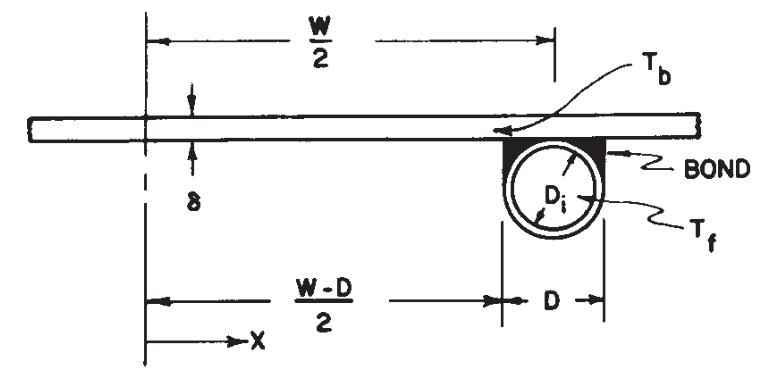
\includegraphics[width=.9\linewidth]{./pictures/collector-tube-dimension.png}
\end{center} 


สมการการอนุรักษ์พลังงานสามารถเขียนอธิบายสมดุลของการถ่ายเทความร้อนได้ดังนี้
\begin{center}
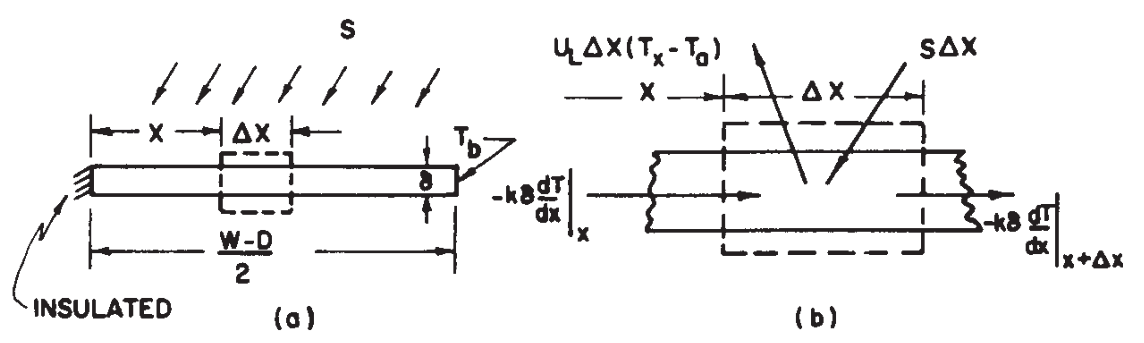
\includegraphics[width=.9\linewidth]{./pictures/collector-tube-dimension-2.png}
\end{center}

\begin{gather*}
  S \Delta x - U_{L} \Delta x (T - T_{a}) + \left. \left( -k \delta \frac{dT}{dx} \right) \right|_{x} - \left. \left( -k\delta \frac{dT}{dx} \right)\right|_{x + \Delta x} = 0 \\
  \frac{d^{2}T}{dx^{2}} = \frac{U_{L}}{k\delta}\left(T - T_{a} - \frac{S}{U_{L}}\right)
\end{gather*}

\begin{description}
\item[{\(S\)}] absorbed solar radiation = \(\alpha I_t\)
\end{description}
\begin{itemize}
\item Using boundary conditions

\begin{enumerate}
\item Symmetry at the centerline: \(\dfrac{dT}{dx} \Bigr|_{x=0} = 0\)
\item Known base temperature: \(T \bigr|_{x=(W-D)/2} = T_b\)
\end{enumerate}

\item Solution takes the form
\begin{align*}
  T = C_{1} \sinh mx + C_{2} \cosh mx + T_{a} + \frac{S}{U_{L}}
\end{align*}

Where \(m = \sqrt{\dfrac{U_L}{k\delta}}\)

\item Substitute boundary conditions give
\begin{align*}
  C_1 &= 0 \\
  T_{b} &= C_{2} \cosh m(W-D)/2 + T_{a} + \frac{S}{U_{L}} \\
  C_{2} &= \frac{T_{b} - T_{a} - S/U_{L}}{\cosh m(W-D)/2}
\end{align*}
\end{itemize}

The temperature distribution takes the form

\begin{align*}
  T &= \frac{T_{b} - T_{a} - S/U_{L}}{\cosh m(W-D)/2}\cosh mx + T_{a} + S/U_{L} \\
  \frac{T - T_{a} - S/U_{L}}{T_{b} - T_{a} - S/U_{L}} &= \frac{\cosh mx}{\cosh m(W-D)/2}
\end{align*}

\begin{itemize}
\item Energy conducted to tube per unit lenth of flow is
\end{itemize}
\begin{align*}
  q_{fin}^{\prime} &= -k\delta\frac{dT}{dx} \Bigr|_{x=(W-D)/2} \\
                   &= \left( \frac{k\delta m}{U_{L}} \right)[S - U_{L}(T_{b}- T_{a})]\tanh \frac{m(W-D)}{2}
\end{align*}

\begin{itemize}
\item Substitute \(m = \sqrt{\dfrac{U_L}{k\delta}}\) to evaluate the energy collection
\begin{align*}
  q_{fin}^{\prime} &= (W - D)[S - U_{L}(T_{b} - T_{a})] \frac{\tanh m(W-D)/2}{m(W-D)/2} \\
                 &= (W - D)[S - U_{L}(T_{b}-T_{a})]\eta_f
\end{align*}

where \(\eta_{f} = \dfrac{\tanh m(W-D)/2}{m(W-D)/2}\) is fin efficiency

\begin{itemize}
\item Energy collected from the region above the tube is
\end{itemize}
\begin{align*}
  q_{tube}^{\prime} &= D[S - U_{L}(T_{b} - T_{a})]
\end{align*}

\begin{itemize}
\item Energy collected for the tube AND fin per flow length is
\end{itemize}
\begin{align*}
  q_{u}^{\prime} &= [(W-D)\eta_f + D][S - U_{L}(T_{b}-T_{a})]
\end{align*}

\begin{description}
\item[{\(q_u^{\prime}\)}] useful heat from collector = solar collected - heat loss
\end{description}
\end{itemize}

\section{Useful Heat Gain Transfer to Fluid}
\label{sec:orgc12a9bc}
\begin{itemize}
\item Solar energy collected = energy transferred to working fluid
\begin{align*}
  q_{u}^{\prime} &= h_{fi}\pi D_{i}(T_{b} - T_{f})
\end{align*}

\begin{description}
\item[{\(h_{fi}\)}] heat transfer coefficient between fluid and tube
\item[{\(D_i\)}] internal tube diameter
\end{description}

\item Substitute other parameters for \(T_b\), we have
\begin{align*}
  q_{u}^{\prime} &= WF^{\prime}[S - U_{L}(T_{f} - T_{a})]
\end{align*}

where the collector efficiency factor \(F^{\prime}\) is
\begin{align*}
  F^{\prime} &= \frac{1/U_{L}}{W\left[ \dfrac{1}{U_{L}[D + (W-D)\eta_f]} + \dfrac{1}{\pi D_{i} h_{fi}} \right]}
\end{align*}

\begin{description}
\item[{\(F^{\prime}\)}] ratio between actual collector's power to power of ideal collector whose temp is \(T_f\)
\end{description}
\end{itemize}

\subsubsection{Example: Calculate Collector Efficiency Factor}
\label{sec:org48eb090}

Given the following data

\begin{center}
\begin{tabular}{lrl}
Overall loss coeff \(U_L\) & 8 & W/m\(^2\text{K}\)\\[0pt]
Tube spacing \(W\) & 150 & mm\\[0pt]
Tube diameter \(D\) & 10 & mm\\[0pt]
Plate thickness \(\delta\) & 0.5 & mm\\[0pt]
Plate thermal conductivity \(k\) & 385 & W/m\(^2\text{K}\)\\[0pt]
Heat transfer coeff inside tube \(h_{fi}\) & 300 & W/m\(^2\text{K}\)\\[0pt]
\end{tabular}
\end{center}

\subsubsection{Solution: Calculate Collector Efficiency Factor}
\label{sec:org41cd990}

First, we need to calculate fin efficiency \(\eta_f\)
\begin{align*}
  m &= \left( \frac{8}{385(0.0005)} \right)^{1/2} = 6.45 \\
  \eta_f &= \frac{\tanh[6.45(0.15 - 0.01)/2]}{6.45(0.15 - 0.01)/2} \\
    &= 0.937
\end{align*}

We can now calculate the collector efficiency factor \(F^{\prime}\)
\begin{align*}
  F^{\prime} &= \frac{1/8}{0.15\left[ \dfrac{1}{8[0.01 + (0.15 - 0.01)0.937]} + \dfrac{1}{\pi(0.01)(300)} \right]} \\
             &= 0.841
\end{align*}


\section{Heat Transfer in Internal Flow}
\label{sec:org17c25cd}

\begin{itemize}
\item Useful gain per flow length is transferred to working fluid
\end{itemize}

\begin{center}
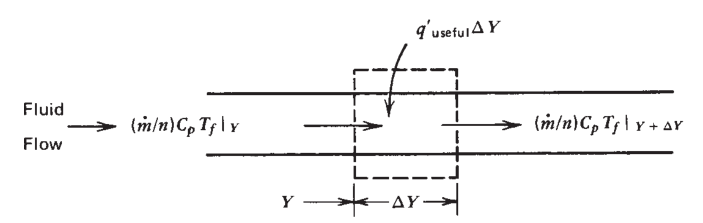
\includegraphics[width=\textwidth]{./pictures/energy-balance-fluid-element.png}
\end{center}

\begin{itemize}
\item Consider energy balance on the fluid element
\end{itemize}
\begin{align*}
  \left( \frac{\dot{m}}{n} \right) C_{p}T_{f} \Biggr|_{y} - \left(\frac{\dot{m}}{n}\right) C_{p}T_{f}\Biggr|_{y+\Delta y}  + \Delta y q_{u}^{\prime} &= 0
\end{align*}

\begin{itemize}
\item As \(\Delta y \rightarrow 0\), we have
\end{itemize}

\begin{align*}
  \dot{m}C_{p}\frac{dT_{f}}{dy} - nWF^{\prime}[S - U_{L}(T_{f}- T_{a})] &= 0
\end{align*}

\begin{itemize}
\item Take inlet fluid temperature = \(T_{fi}\)
\end{itemize}
\begin{align*}
  \frac{T_{f} - T_{a} - S/U_{L}}{T_{fi} - T_{a} - S/U_{L}} = \exp\left( -\frac{U_{L}nWF^{\prime}y}{\dot{m}C_{p}} \right)
\end{align*}

\begin{itemize}
\item Collector heat removal factor (\(F_R\)) = ratio of actual useful energy gain to ideal useful energy gain if the collector were at fluid inlet temperature \(T_{fi}\)

$$ F_R = \frac{\dot{m}C_p(T_{fo} - T_{fi})}{A_c [S - U_L(T_{fi} - T_a)]} $$

\item The equation can be rearranged so that
\end{itemize}
\begin{align*}
  F_R &= \frac{\dot{m}C_p}{A_{c}U_{L}}\left[\frac{(T_{fo} - T_{fi})}{S/U_{L} - (T_{fi} - T_a)}\right] \\
      &= \frac{\dot{m}C_p}{A_{c}U_{L}}\left[\frac{(S/U_{L} - (T_{fo} - T_{a})) - (S/U_{L} - (T_{fo} - T_{a}))}{S/U_{L} - (T_{fi} - T_a)}\right] \\
      &= \frac{\dot{m}C_p}{A_{c}U_{L}}\left[1 - \frac{S/U_{L} - (T_{fo} - T_{a})}{S/U_{L} - (T_{fi} - T_a)}\right] \\
      &= \frac{\dot{m}C_{p}}{A_{c}U_{L}} \left[1 - \exp\left( - \frac{A_{c}U_{L}F^{\prime}}{\dot{m}C_{p}} \right)\right]
\end{align*}

\begin{itemize}
\item Collector flow factor, \(F^{\prime\prime}\) is defined as
\end{itemize}
\begin{align*}
  F^{\prime\prime} = \frac{F_{R}}{F^{\prime}} &= \frac{\dfrac{\text{actual fluid heat gain}}{\text{ideal fluid heat gain at }T_f}}{\dfrac{\text{actual absorbed energy}}{\text{ideal fluid heat gain at }T_f}} \\
                   &= \frac{\text{actual fluid heat gain}}{\text{actual absorbed energy}} \\
                   &= \frac{\dot{m}C_{p}}{A_{c}U_{L}F^{\prime}} \left[1 - \exp\left( - \frac{A_{c}U_{L}F^{\prime}}{\dot{m}C_{p}} \right)\right]
\end{align*}

\begin{itemize}
\item \(F^{\prime\prime}\) only depends on dimensionless collector mass flow rate \(\dfrac{\dot{m}C_{p}}{A_{c}U_{L}F^{\prime}}\).
\end{itemize}


\begin{itemize}
\item Collector Efficiency, \(\eta\)

\item Actual fluid useful heat gain compared to incident solar radiation
\begin{align*}
  \eta &= \frac{q_{u}}{I_{T}} = \frac{Q_{u}}{I_{T}A_{c}}
\end{align*}
\end{itemize}
\subsubsection{Example: Solar Collectors in KK, Thailand}
\label{sec:orge1a9d95}

คำนวณพลังงานเพิ่มที่ได้รับและประสิทธิภาพของแผงรับพลังงานแสงอาทิตย์ 10 แผ่นซึ่งตั้งอยู่ใกล้ จ.ขอนแก่น แผ่นถูงตั้งที่มุม tilt 16.4° ไปทางทิศใต้ สมมุติว่าสัมประสิทธิ์การสูญเสียความร้อนเป็น 0.841 น้ำไหลผ่านแผ่นรับแสงอาทิตย์ขนาด 1 \texttimes{} 2-m ด้วยอัตรา 0.03 kg/s ด้วยอุณหภูมิขาเข้า 40°C ค่า absorptivity เป็น 0.8

\subsubsection{Solution: Solar Collectors in KK, Thailand}
\label{sec:org5abf90f}

First, calculate dimensionless collector mass flow rate
\begin{align*}
  \frac{\dot{m}C_{p}}{A_{c}U_{L}F^{\prime}} &= \frac{0.03(4190)}{2(8)(0.841)} = 9.35
\end{align*}

Collector flow factor can then be calculated
\begin{align*}
  F^{\prime\prime} &= 9.35 \left[ 1 - \exp \left( - \frac{1}{9.35} \right) \right] \\
                   &= 0.948
\end{align*}


The heat removal factor is
\begin{align*}
  F_{R} &= F^{\prime}F^{\prime\prime} = 0.841(0.948) = 0.797
\end{align*}

Average loss rate for the hour of 10 - 11, based on inlet temperature of 40 C, is
\begin{align*}
  q_{loss} = U_{L}(T_{fi} - T_{a}) = 8(40 - 37)(3600) = 8.64 \times 10^{4} \text{ J/m}^{2}\text{h}
\end{align*}

From spreadsheet calculation, radiation from 10 - 11 on surface \(\beta = 16.4^{\circ}\) to the south is 3.95 MJ/m\(^2\). Average useful energy gain per collector area is
\begin{align*}
  q_{u} &= F_R(S - q_{loss}) = 0.797(0.8(395) - 8.64) \times 10^{4} = 245  \times 10^4 \text{ J/m}^{2}\text{h}
\end{align*}

\subsubsection{Solution: Solar Collectors in KK, Thailand}
\label{sec:org508affe}

The collector efficiency for 10 - 11 is
\begin{align*}
  \eta &= \frac{Q_{u}}{I_{T}A_{C}} = \frac{q_{u}}{I_{T}} = \frac{2.45}{3.95} \\
       &= 0.62
\end{align*}

\subsubsection{Solution: Table of by-the-hour Results}
\label{sec:org3a5f7bd}

\begin{center}
\begin{tabular}{crccccc}
\toprule
Time & \(T_a\) & \(I_T\) & \(q_{loss}\) & \(q_u\) & \(\eta\)\\[0pt]
\midrule
6 & 28 & 0.00 & 0.35 & 0.00 & 0.00\\[0pt]
7 & 29 & 0.23 & 0.32 & 0.00 & 0.00\\[0pt]
8 & 30 & 0.94 & 0.29 & 0.37 & 0.39\\[0pt]
9 & 32 & 1.52 & 0.23 & 0.79 & 0.52\\[0pt]
10 & 35 & 3.05 & 0.14 & 1.83 & 0.60\\[0pt]
11 & 37 & 3.95 & 0.09 & 2.45 & 0.62\\[0pt]
12 & 38 & 4.44 & 0.06 & 2.79 & 0.63\\[0pt]
13 & 38 & 4.39 & 0.06 & 2.76 & 0.63\\[0pt]
14 & 37 & 3.82 & 0.09 & 2.37 & 0.62\\[0pt]
15 & 35 & 2.87 & 0.14 & 1.72 & 0.60\\[0pt]
16 & 34 & 1.79 & 0.17 & 1.00 & 0.56\\[0pt]
17 & 33 & 0.87 & 0.20 & 0.39 & 0.45\\[0pt]
18 & 32 & 0.23 & 0.23 & 0.00 & 0.00\\[0pt]
\midrule
Total &  &  &  & 16.47 & \\[0pt]
\bottomrule
\end{tabular}
\end{center}

\subsubsection{Summary}
\label{sec:orgb9fcce1}

\begin{itemize}
\item Most used type of collectors
\item Best up to 100 C
\item Improvement in machining such as laser and ultrasonic welding can improve quality of welds
\item Careful design of length, width, tube spacing is crucial to achieve optimal performances
\end{itemize}

\chapter{เทอร์โมอิเล็กทริก}
\label{sec:orged353c0}
เทอร์โมอิเล็กทริกซิตี้ (thermoelectricity) เป็นการแปลงพลังงานโดยตรงจากความร้อนไปเป็นพลังงานไฟฟ้า
ซึ่งสารที่สามารถแปลงพลังงานด้วยวิธีนี้ได้เรียกว่าวัสดุเทอร์โมอิเล็กทริก
ซึ่งเทคโนโลยีนี้มีความน่าสนใจเนื่องจากในปัจจุบันในโลกของเรายังมีแหล่งพลังงานความร้อนราคาถูกอยู่มาก
ไม่ว่าจะเป็นแหล่งพลังงานพลังงานแสงอาทิตย์ หรือพลังงานความร้อนเหลือใช้จากกระบวนการทางอุตสาหกรรมต่างๆ
โดยในการแปลงพลังงานที่เกิดขึ้นนั้นเกิดขึ้นจากปรากฏการณ์เทอร์โมอิเล็กทริก
(thermoelectric effect)
ซึ่งสามารถแบ่งย่อยออกเป็นปรากฏการณ์ซึ่งเกิดขึ้นพร้อมกัน 3
อย่างดังต่อไปนี้

\section{ปรากฏการณ์ซีเบ็ก}
\label{sec:orgae75c47}
เทอร์โมอิเล็กทริกซิตี้เป็นปรากฏการณ์การเกิดศักย์ไฟฟ้าขึ้นบนตัวนำหรือสารกึ่งตัวนำที่มีอุณหภูมิเปลี่ยนไป
โดยมีหลักการมาจากการแพร่ (diffusion) ของพาหะของประจุ (charge carrier)
ในสารเมื่อได้รับความร้อน
โดยในสารตัวนำและกึ่งตัวนำทั่วไปจะมีทั้งอิเลกตรอนอิสระ (free electrons)
ซึ่งมีประจุลบ และหลุม (holes) ซึ่งมีประจุบวก เมื่อวัสดุได้รับความร้อน
พาหะในสารจะแพร่ตัวออกไปยังบริเวณที่มีอุณหภูมิต่ำกว่า
การสะสมของพาหะเหล่านี้ทำให้เกินศักย์ไฟฟ้าขึ้น

เมื่อนำไปต่อกับภาระภายนอกจะทำให้มีการไหลของกระแสไฟฟ้าเกินขึ้นได้

สารทุกชนิดมีความสามารถในการสร้างศักย์ไฟฟ้าจากการแพร่ของพาหะประจุที่ต่างกัน
โดยค่าความสามารถนี้เรียกว่า ค่าสัมประสิทธิ์ซีเบ็ก (Seebeck Coefficient)
ซึ่งอธิบายความสามารถศักย์ไฟฟ้าที่เกิดจากอุณหภูมิที่แตกต่างได้ดังนี้

\begin{equation}
\label{eq:org950289c}
  V = \int_{T_L}^{T_H} \left( S_p - S_n \right) dT = \int_{T_L}^{T_H} S_{pn} dT
\end{equation}

ซึ่งหากเราสมมติว่าค่าสัมประสิทธิ์นี้เป็นอิสระจากอุณหภูมิ จะสามารถเขียนสมการ \ref{eq:org950289c} ใหม่ได้ว่า

\[V = S_{pn} \Delta T = S_{pn} \left( T_H - T_L \right)\]

โดยค่าสัมประสิทธิ์สำหรับวัสดุทั่วไปที่มีสมบัติเป็นวัสดุเทอร์โมอิเล็กทริกได้มีดังนี้

\begin{center}
\begin{tabular}{lr}
\toprule
Material & \(S\), V / K \(\times\) 10\(^{\text{-6}}\)\\[0pt]
\midrule
Aluminum & -0.2\\[0pt]
Constantan & -47\\[0pt]
Copper & 3.5\\[0pt]
Iron & 13.6\\[0pt]
Platinum & -5.2\\[0pt]
Germanium & 375\\[0pt]
Silicon & -455\\[0pt]
Bismuth Telluride & 200\\[0pt]
\bottomrule
\end{tabular}
\end{center}

อย่างไรก็ดี ประสิทธิภาพของเทอร์โมอิเล็กทริกจากวัสดุหนึ่งๆนั้นไม่ได้ขึ้นอยู่กับค่าสัมประสิทธิ์ซีเบ็กเพียงอย่างเดียว เนื่องจากลักษณะการทำงานและการต่อเชื่อมของเทอร์โมอิเล็กทริกกับวงจรไฟฟ้านั้นเป็นเหมือนแบตเตอรี่ชนิดหนึ่ง ซึ่งสามารถเขียนอธิบายเป็นวงจรได้ดังรูปที่ \ref{org0480276}

\begin{figure}[h]
  \centering
  \begin{tikzpicture}
    \draw (0,2) to [V_=$V_{OC}$] ++(90:-2) to [short, -*] ++ (0:2) to [short] ++ (0:2) to [R,l_=$R_L$] ++ (90:2) to [short, -*] ++ (180:2) to [R=$R_{TEG}$, -*] ++ (180:2);
    \node [yshift=1cm, xshift=2.5mm, draw, dashed, rounded corners=4mm, minimum width=3.5cm, minimum height=3.5cm](teg){};
    \node [below=of teg, yshift=1cm] {Thermoelectric Generator};
  \end{tikzpicture}
\caption{\label{org0480276}ภาพวงจรแสดงคุณสมบัติของเครื่องผลิตไฟฟ้าเทอร์โมอิเล็กทริก}
\end{figure}

ซึ่งจะเห็นว่าเทอร์โมอิเล็กทริกเป็นเหมือนแหล่งศักย์ไฟฟ้า (\(V\))
ที่มีความต้านทานภายใน (\(R_{TEG}\))

\begin{gather*}
  V_L = S_{pn}\Delta T - iR_{int} \\
  R_{int} = R_p + R_n
\end{gather*}

นอกจากนี้ อีกวิธีที่สามารถใช้เพิ่มกระแสไฟฟ้าก็คือการต่อคู่เทอร์โมอิเล็กตริกแบบอนุกรมเพื่อเพิ่มแรงดันไฟฟ้า เช่นเดียวกับการต่อแบตเตอรี่ AA หรือ AAA หลายก้อนในอุปกรณ์ไฟฟ้าแบบพกพาทั้งหลาย ถ้าสมมุติว่าต่อเทอร์โมอิเล็กทริกทั้งหมด \(m\) คู่ จะได้สมการไฟฟ้าว่า

\begin{gather*}
  V = m S_{pn} \Delta T \\
  R_{teg} = m R_{int} \\
  V_L = m S_{pn} \Delta T - i mR_{int}\end{gather*}

การที่จะสามารถดึงกำลังไฟฟ้าจากเทอร์โมอิเล็กทริกมาใช้ให้ได้มากที่สุดจึงจำเป็นจะต้องมีการปรับความต้านทานภาระ (Load resistance, \(R_L\)) ให้เหมาะสม เพื่อให้มีการสูญเสียไปกับความต้านทานภายในของเทอร์โมอิเล็กทริกให้น้อยที่สุด ซึ่งความต้านทานภาระที่เหมาะสมนี้สามารถหาได้จากสมการดังนี้

\begin{gather*}
  P_L = iV_L = i m S_{pn} \Delta T - i^2 m R_{int} \\
  \frac{d P_L}{d i } = 0 = m(S_{pn} \Delta T - 2 i R_{int}) \\
  i_{max P} = \dfrac{S_{pn} \Delta T}{2 R_{int}} \\
  i = \dfrac{V}{R} = \dfrac{ m S_{pn} \Delta T }{ m R_{int} + R_L } \\
  R_L = m R_{int}\end{gather*}

หมายความว่า ความต้านทานภาระควรจะเท่ากับความต้านทานภายใน ซึ่งนี่เรียกว่า
load matching
ซึ่งเป็นวิธีการที่ใช้ได้กับการผลิตไฟฟ้าด้วยกระบวนการอื่นๆได้เช่นกัน

\section{ปรากฏการณ์เพลเทียร์}
\label{sec:org33ad7b5}
ปรากฏการณ์เพลเทียร์เป็นปรากฏการณ์ที่ตรงกันข้ามกับปรากฏการณ์ซีเบ็ก  ในกรณีของปรากฏการณ์ซีเบ็กนั้น ผลต่างของอุณหภูมิสร้างให้เกิดความต่างศักย์และกระแสไฟฟ้า ส่วนปรากฏการณ์เพลเทียร์เป็นการสร้างผลต่างของอุณหภูมิเมื่อมีกระแสไฟฟ้าไหลผ่าน เปรียบเทียบได้กับกรณีของปรากฏการณ์แม่เหล็กไฟฟ้าในมอเตอร์ ซึ่งเมื่อใส่กระแสไฟฟ้าเข้าไปในตัวนำซึ่งอยู่ในสนามแม่เหล็กจะทำให้เกิดการหมุน ในทางตรงกันข้าม ถ้านำตัวนำไปหมุนภายในสนามแม่เหล็กก็จะทำให้เกิดกระแสไฟฟ้าเหนี่ยวนำขึ้นเช่นกัน

ประโยชน์ของปรากฏการณ์นี้สามารถนำไปประยุกต์ใช้ในการทำความเย็น โดยตัวทำความเย็นที่อาศัยหลักการนี้เรียกว่าตัวทำความเย็นเพลเทียร์ (Peltier cooler) โดยอัตราการกำจัดความร้อนสามารถคำนวณได้จาก

\begin{equation}
  Q_{peltier} = m S_{pn} T_H i
\end{equation}

ซึ่งตัวทำความเย็นนี้มีจุดเด่นเช่นเดียวกับตัวผลิตไฟฟ้าเทอร์โมอิเลกตริก
นั่นคือไม่มีชิ้นส่วนที่เคลื่อนไหว
จึงทำให้มีอัตราการสึกหรอน้อยกว่าระบบทำความเย็นแบบใช้สารทำความเย็นทั่วไป
ลดความซับซ้อนของระบบทำความเย็น รวมถึงลดค่าซ่อมแซมและดูแลรักษาได้
แม้ปัจจุบันประสิทธิภาพจะยังไม่ดีเท่ากับระบบทำความเย็นแบบทั่วไป
และมีราคาสูงเมื่อเทียบกับอัตราการกำจัดความร้อน
แต่ก็ได้มีการนำมาใช้ในกรณีที่มีพื้นที่การติดตั้งจำกัด
เช่นระบบทำความเย็นในหน่วยประมวลผล (processor) ของคอมพิวเตอร์

\section{ปรากฏการณ์ทอมสัน}
\label{sec:org086296f}
ดังที่ได้กล่าวมาแล้วในส่วนของปรากฏการณ์เทอร์โมอิเลกทริก
ค่าสัมประสิทธิ์ซีเบ็กของแต่ละวัสดุนั้นมักจะแปรผันกับอุณหภูมิ
ดังนั้นในกรณีที่วัสดุมีอุณหภูมิที่ไม่สม่ำเสมอ
ค่าสัมประสิทธิ์ซีเบ็กก็อาจจะไม่สม่ำเสมอได้เช่นกัน
และเมื่อมีกระแสไฟฟ้าไหลผ่านวัสดุนี้ก็จะทำให้มีการเกิดปรากฏการณ์เพลเทียร์เกิดขึ้นได้
ปรากฏการณ์นี้เรียกว่า'ปรากฏการณ์ทอมสัน' ตั้งตามชื่อของลอร์ดเคลวิน
(ชื่อจริง William Thomson)
ซึ่งได้ทำนายการเกิดปรากฏการณ์นี้ในตัวนำที่มีอุณหภูมิไม่สม่ำเสมอดังที่ได้กล่าวมาแล้วในส่วนของปรากฏการณ์เทอร์โมอิเลกทริก
ค่าสัมประสิทธิ์ซีเบ็กของแต่ละวัสดุนั้นมักจะแปรผันกับอุณหภูมิ
ดังนั้นในกรณีที่วัสดุมีอุณหภูมิที่ไม่สม่ำเสมอ
ค่าสัมประสิทธิ์ซีเบ็กก็อาจจะไม่สม่ำเสมอได้เช่นกัน
และเมื่อมีกระแสไฟฟ้าไหลผ่านวัสดุนี้ก็จะทำให้มีการเกิดปรากฏการณ์เพลเทียร์เกิดขึ้นได้
ปรากฏการณ์นี้เรียกว่า'ปรากฏการณ์ทอมสัน' ตั้งตามชื่อของลอร์ดเคลวิน
(ชื่อจริง William Thomson)
ซึ่งได้ทำนายการเกิดปรากฏการณ์นี้ในตัวนำที่มีอุณหภูมิไม่สม่ำเสมอและทำการทดลองจนสามารถพิสูจน์ได้จริง

ในกรณีที่มีความหนาแน่นกระแสไฟฟ้า \(J\)
ไหลผ่านตัวนำที่มีค่าสัมประสิทธิ์ทอมสัน \(\mathcal{K}\)
อัตราการเกิดความร้อนจะมีค่าเท่ากับ

\[q_{thomson} = - \mathcal{K} J \cdot \nabla T\]

สังเกตว่าในสมการนี้ กำลังความร้อนที่เกิดขึ้นมืหน่วยเป็น W/m\(^3\)
เนื่องจากคุณสมบัติของตัวนำไม่สม่ำเสมอ
กำลังความร้อนจึงไม่คงที่และต้องอาศัยการอินทิเกรตเพื่อหาค่าบนพื้นที่หรือปริมาตร

\section{หลักการทำงานของเทอร์โมอิเลกทริก}
\label{sec:org7d6aa39}
ในระหว่างการทำงานจริงมักมีปรากฏการณ์เทอร์โมอิเลกทริกสองอย่างขึ้นไปเกิดขึ้นพร้อมๆกัน
ดังนั้นจึงมีความจำเป็นที่จะต้องทำความเข้าใจความสัมพันธ์ของปรากฏการณ์ต่างๆและผลที่เกิดขึ้นกับเทอร์โมอิเลกทริก
อย่างไรก็ดี สำหรับในตำราเล่มนี้
จะขอกล่าวถึงความสัมพันธ์เมื่อเทอร์โมอิเลกทริกทำงานที่สถานะคงที่ (steady
state) ซึ่งหมายถึงอุณหภูมิที่จุดต่างๆคงที่
ในที่นี้เราจะพิจารณาที่ด้านร้อนของเทอร์โมอิเลกทริกซึ่งมีการถ่ายเทความร้อนเกิดขึ้นดังต่อไปนี้

\begin{enumerate}
\item ความร้อนจากแหล่งความร้อนเข้าสู่ด้านร้อน \(Q_{in}\)

\item ความร้อนจากปรากฏการณ์การเกิดความร้อนของจูล \(Q_{joule}\)

\[Q_{joule} = i^2 R\]

\item ความร้อนออกจากด้านร้อนไปสู่ด้านเย็นด้วยการนำความร้อน \(Q_{cold}\)

\[Q_{cold} = K \Delta T\]

\item ความร้อนออกจากด้านร้อนด้วยปรากฏการณ์เพลเทียร์ \(Q_{peltier}\)

\[Q_{peltier} = S_{pn} T_H i\]
\end{enumerate}

ที่สถานะคงที่ อัตราการได้รับความร้อนและสูญเสียความร้อนเท่ากัน
ซึ่งอัตราการได้รับความร้อน (\(Q_{in}\)) มาจาก

\[Q_{in} + Q_{joule} = Q_{cold} + Q_{peltier}\]

\begin{align*}
    Q_{in} &=  Q_{cold} + Q_{peltier} - Q_{joule}  \\
    &=  m S_{pn} T_H i +  K\Delta T -  \dfrac{i^2 R_{teg}}{2}
  \end{align*}

กำลังไฟฟ้าที่ผลิตได้ผ่านตัวต้านทานเท่ากับ

\[P_{out} = i^2 R_L\]

ซึ่งเราสามารถเอามาเขียนเป็นสมการประสิทธิภาพความร้อนของ TEG เท่ากับ

\begin{align}
\label{eq:org631700a}
  \eta &= \frac{P_{out}}{Q_{in}} \\
  &= \frac{i^2 R_L}{ m S_{pn} T_H i + K \Delta T - \dfrac{ i^2 R_{teg}}{2}}
\end{align}

กำหนดอัตราส่วน

\begin{equation}
\label{eq:orgc3b5a49}
 Z = \frac{S_{pn}^2}{K_{teg} R_{teg}}
\end{equation}

ซึ่งเรียกว่า figure of merit และแทนค่าเข้าในสมการ \ref{eq:org631700a} จะสามารถเขียนสมการประสิทธิภาพของเทอร์โมอิเลกทริกได้ว่า

\begin{equation}
\label{eq:orge0106ed}
  \eta = \dfrac{ \Delta T }{ 2 T_H + \dfrac{2}{Z} - \dfrac{ \Delta T }{ 2 } }
\end{equation}

จากสมการข้างต้น ที่อุณหภูมิ \(T_H\) และ \(T_L\) ใดๆ ประสิทธิภาพของ TEG
จะสูงสุดเมื่อมีค่า \(Z\) สูง
ซึ่งแปลว่าวัสดุจะต้องมีค่าสัมประสิทธ์ซีเบ็กสูง นำความร้อนได้ไม่ดี
และมีความต้านทานไฟฟ้าต่ำ ซึ่งคุณสมบัติสองอย่างหลังนี้หาได้ยาก
เพราะวัสดุที่เป็นตัวนำไฟฟ้าที่ดี ก็มักจะนำความร้อนได้ดีเช่นกัน
ส่วนวัสดุที่เป็นฉนวนไฟฟ้า ก็มักจะเป็นฉนวนความร้อนด้วย

ประสิทธิภาพของเครื่องยนต์ความร้อนส่วนใหญ่ (นอกจากเครื่องยนต์สันดาปภายใน)
มักจะเปรียบเทียบประสิทธิภาพเป็นสัดส่วนเทียบกับประสิทธิภาพคาร์โนต์ซึ่งเป็นประสิทธิภาพสูงสุดในทางทฤษฎีของเครื่องยนต์ความร้อนใดๆ

\begin{figure}[h]
  \centering
  \begin{tikzpicture}
    \begin{axis} [
      width=\textwidth,
      height=.7\textwidth,
      legend style={at={(0.1,0.9)},
        legend cell align={left},
        anchor=north west,
        fill=none},
      % xtick=data,
      xmin=0,xmax=400,
      ymin=0,ymax=0.6,
      domain=0:400,
      ytick distance=0.1,
      xlabel={ส่วนต่างอุณหภูมิ $\Delta T$},
      ylabel={ประสิทธิภาพความร้อน \%},
      % cycle list/Paired,
      ]
      \addplot {\x / (50 + \x + 273)};
      \addplot {\x / (2*(\x + 50 + 273) + 2*(\x + 273 + 50)/2 - \x/2) };
      \addplot {\x / (2*(\x + 50 + 273) + 2*(\x + 273 + 50)/1 - \x/2) };
      \addplot {\x / (2*(\x + 50 + 273) + 2*(\x +  273 + 50)/0.5 - \x/2) };
      \legend{Carnot, $ZT$ = 2, $ZT$ = 1, $ZT$ = 0.5};
    \end{axis}
  \end{tikzpicture}
\caption{\label{org8ba8193}ประสิทธิภาพความร้อนของ TEG เทียบกับประสิทธิภาพคาร์โนต์}
\end{figure}

จากรูป \ref{org8ba8193} จะเห็นได้ว่าแม้ที่ \(ZT = 2\) ประสิทธิภาพของเทอร์โมอิเลกทริกยังมีค่าอยู่ที่ประมาณ 10\% - 20\% ของประสิทธิภาพคาร์โนต์ ซึ่งนับว่ายังต่ำมากเมื่อเทียบกับเครื่องยนต์สันดาปภายในทั่วไปซึ่งมีประสิทธิภาพประมาณ 50\% - 80\% ของประสิทธิภาพคารโนต์

\section{{\bfseries\sffamily TODO} วัสดุเทอร์โมอิเลกทริก}
\label{sec:orgd30faa7}
จากสมการ \ref{eq:orgc3b5a49}
จะเห็นได้ว่าประสิทธิภาพของเทอร์โมอิเลกทริกขึ้นอยู่กับค่าการนำไฟฟ้า
การนำความร้อน และค่าสัมประสิทธิ์ซีเบ็ก
การที่จะปรับปรุงประสิทธิภาพสามารถทำได้โดยใช้วิธีการขั้นสูงในการปรับปรุงคุณสมบัติของวัสดุหรือใช้วัสดุที่มีขนาดเล็กมาก
\ldots{}
วัสดุที่ได้รับความสนใจและได้ถูกนำมาประยุกต์ใช้เป็นเครื่องกำเนิดไฟฟ้าเทอร์โมอิเลกทริกได้แก่

\begin{enumerate}
\item สารประกอบแชลโคเจนของบิสมัท (Bismuth Chalcogenides)

สารประกอบในกลุ่มนี้อย่างบิสมัทเทลลูไรด์ (\(\ce{Bi2Te3}\))
และบิสมัทซีลีไนด์ (\(\ce{Bi2Se3}\))
ถือเป็นเทอร์โมอิเลกทริกที่มีประสิทธิภาพสูงที่สุดที่อุณหภูมิห้องกลุ่มหนึ่ง
โดยที่มีค่า figure of merit (\(ZT\)) อยู่ที่ประมาณ 0.8 - 1.0

บิสมัทเทลลูไรด์เป็นวัสดุเทอร์โมอิเลกทริกที่อุณหภูมิห้องที่ดี
และสามารถนำมาใช้สำหรับการทำความเย็นได้ที่อุณหภูมิประมาณ 300 K (27 C)
สารประกอบเหล่านี้ได้มาจากการผลิตผลึกเดี่ยวด้วยวิธีของ Czochralski
บางส่วนถูกผลิตโดยการเย็นตัวจากของเหลวหรือเทคนิคการขึ้นรูปโลหะผง
วัสดุอย่างหลังนี้จะมีประสิทธิภาพต่ำกว่าแบบผลึกเดี่ยว
แต่จะมีคุณสมบัติทางกลที่ดีกว่าและทนต่อความบกพร่องทางโครงสร้างและสิ่งแปลกปลอมได้ดีกว่า
การสร้างความหนาแน่นของประจุไฟฟ้าสามารถทำได้โดยเพิ่มสารบิสมัทหรือเทลลูเรียมเข้าไปในสารประกอบให้เกินความไม่สมดุล
หรือการเพิ่มสารแปลกปลอมจำพวกฮาโลเจนเข้าไป
การใช้สารประกอบเทลลูไรด์ยังไม่สามารถใช้ในวงกว้างได้เนื่องจากเทลลูเรียมมีพิษและเป็นธาตุที่หาได้ยาก

\item ตะกั่วเทลลูไรด์ (\(\ce{PbTe}\))

งานวิจัยโดย Heremans และคณะแสดงให้เห็นว่าตะกั่วเทลลูไรด์ที่โดปด้วยแทลเลี่ยมมีค่า figure of merit สูงถึง 1.5 ที่อุณหภูมิ 773 K \citeprocitem{1}{[1]} นอกจากนี้ งานวิจัยโดย Snyder และคณะได้รายงานว่าสามารถสร้างเทอร์โมอิเลกทริกที่มีค่า \(ZT\) = 1.4 ที่อุณหภูมิ 750 K โดยใช้ตะกั่วเทลลูไรด์ และยังสร้างเทอร์โมอิเลกทริกที่มี \(ZT\) = 1.8 ที่อุณหภูมิ 850 K โดยใช้ตะกั่วเทลลูไรด์ซีลีไนด์ที่โดปด้วยโซเดียม (sodium-doped \(\ce{PbTe_{1-x}Se_x}\)) \citeprocitem{2}{[2]}

มีรายงานจากงานวิจัยโดย Biswas
และคณะว่าสามารถแปลงพลังงานความร้อนเหลือทิ้งเป็นไฟฟ้าด้วยประสิทธิภาพ 15 - 20\% (เทอร์โมอิเลกทริกมีค่า \(ZT\) ถึง 2.2) ซึ่งเป็นค่าที่สูงที่สุดที่เคยมีการรายงาน \citeprocitem{3}{[3]}

\item สารประกอบคลาเทรตอนินทรีย์ (Inorganic Clathrates)

กลุ่มสารประกอบเหล่านี้มีสูตรทางเคมีโดยทั่วไปว่า \(\ce{A_xB_yC_{46-y}}\) สำหรับกลุ่มที่ 1 และ \(\ce{A_xB_yC_{136-y}}\) สำหรับกลุ่มที่ 2 โดยที่ B และ C เป็นธาตุในหมู่ III และ IV ซึ่งประกอบตัวเป็นเหมือนกรอบล้อม A ไว้
\end{enumerate}

\section{การออกแบบเทอร์โมอิเลกทริก}
\label{sec:org1927320}
การเพิ่มประสิทธิภาพของการผลิตไฟฟ้าจากเทอร์โมอิเลกทริกสามารถทำได้โดยการออกแบบขนาดวัสดุหรือเพิ่มประสิทธิภาพการถ่ายเทความร้อนของด้านร้อนและเย็นของเทอร์โมอิเลกทริก

\subsection{ตัวอย่าง: การวิเคราะห์เทอร์โมอิเลกทริก}
\label{sec:org0caf02d}
เทอร์โมอิเลกทริกทำมาจาก \(\ce{PbTe-Bi2Te3}\) ซึ่งมีคุณสมบัติดังต่อไปนี้

\begin{table}[htbp]
\label{tab:orgbc6a531}
\centering
\begin{tabular}{lrr}
\toprule
Properties & P-type & N-type\\[0pt]
\midrule
Seebeck coefficient \(10^{-6}\) & 300 & -100\\[0pt]
Electrical resistivity \(10^{-6}\) & 9 & 10\\[0pt]
Thermal conductiviity & 1.2 & 1.4\\[0pt]
\bottomrule
\end{tabular}
\end{table}

ขาจากวัสดุทั้งสองชนิดมีพิ้นที่หน้าตัด (16 mm\(^2\))และความยาว (4 mm)
เท่ากัน ที่สภาวะคงที่อุณหภูมิด้านร้อนเท่ากับ 200 C และด้านเย็นเท่ากับ 50
C จงคำนวณหา

\begin{enumerate}
\item ค่า \(Z\) ของเทอร์โมอิเลกทริกนี้

\item กำลังสูงสุดที่เทอร์โมอิเลกทริกนี้ผลิตได้

\item ประสิทธิภาพของเทอร์โมอิเลกทริกนี้
\end{enumerate}

\subsection{เฉลย: การวิเคราะห์เทอร์โมอิเลกทริก}
\label{sec:org75d7247}
\begin{enumerate}
\item ค่า \(Z\) สามารถคำนวณได้จากสมการ
\(Z = \dfrac{S_{pn}^2}{K_{teg} R_{teg}}\)

\begin{align*}
S_{pn} &= S_p - S_n =0.0003- (-0.0001) \\
&= 0.0004\\
K_{teg} &= K_p + K_n = \frac{\kappa_p A}{L} + \frac{\kappa_n A}{L} \\
&= \frac{ \num{1.6e-05}}{ \num{4.00e-03}} \left(1.2+1.4\right) \\
&=0.0104\\
R_{teg} &= R_p + R_n = \frac{\rho_p L}{A} + \frac{\rho_n L}{A} \\
&= \frac{0.004}{1.6e-05} \left(\num{1.2}+\num{1.4}\right) \\
&=0.00475\\
Z &= \frac{Z^2}{K_{teg}R_{teg}} \\
&=0.00324
\end{align*}

\item กำลังสูงสุดที่ TEG สามารถผลิตได้มาจากการ load matching โดยการใช้
\(R_L = R_{teg}\)

\begin{align*}
P_L &= i V_L \\
&= i \left( S_{pn} \Delta T - i^2 R_{teg} \right) \\
&= \frac{S_{pn} \Delta T}{2 R_{teg}} \left( S_{pn} \Delta T -  \frac{S_{pn} \Delta T}{2 R_{teg}} R_{teg} \right) \\
&= \frac{ S_{pn}^2 \Delta T^2 }{4 R_{teg}} \\
&= \frac{0.0004^2 (200 - 50)^2}{4 (0.00475)} \\
&=\num{1.89e-01}
\end{align*}

\item ประสิทธิภาพของ TEG สามารถคำนวณได้จากสมการ
\ref{eq:orge0106ed}

\begin{align*}
\eta &= \frac{ \Delta T }{ 2 T_H + \dfrac{2}{Z} - \dfrac{ \Delta T }{ 2 } } \\
&= \frac{200-50}{ 2(200 + \frac{2}{0.00324} + \frac{200-50}{2}} \\
&=0.159
\end{align*}
\end{enumerate}

\chapter{เซลล์เชื้อเพลิง}
\label{sec:orge1f4467}

\epigraph{ไม่สำคัญหรอกว่าคุณจะสามารถหาคัวนำยิ่งยวดที่อุณหภูมิสูงหรือเซลล์เชื้อเพลลิงได้หรือไม่ ยังไงมันก็จะอยู่ในความสนใจของทุกคนเสมอ เพราะถ้าทำได้เมื่อใด มันก็จะมีประโยชน์มากมายมหาศาล It doesn't matter whether you can or cannot achieve high temperature superconductivity or fuel cells, they will always be on the list because if you could achieve them they would be extremely valuable.}{Martin Fleischmann}

เซลล์เชื้อเพลิงเป็นอุปกรณ์ที่อาศัยกระบวนการเปลี่ยนแปลงพลังงานจากพลังงงานเคมีไปเป็นพลังงานไฟฟ้าโดยตรง
ซึ่งแตกต่างจากการใช้เครื่องยนต์ในการปั่นไฟซึ่งเปลี่ยนพลังงานเคมีไปเป็นพลังงานความร้อนไปเป็นพลังงานกลแล้วจึงเป็นพลังงานไฟฟ้าในที่สุด
เนื่องจากเซลล์เชื้อเพลิงมีการเปลี่ยนแปลงพลังงานเพียงขั้นตอนเดียว
และยังไม่มีขั้นตอนการเปลี่ยนแปลงพลังงานความร้อน
จึงทำให้สามารถทำให้กระบวนการมีประสิทธิภาพสูงกว่าวิธีเปลี่ยนแปลงพลังงานเคมีในรูปแบบอื่น

จุดเด่นของเซลล์เชื้อเพลิงคือสามารถนำการแลกเปลี่ยนอิเลกตรอนที่เกิดขึ้นในปฏิกิริยาการสันดาปมาใช้ได้โดยตรง
ซึ่งปฏิกิริยาที่เกิดขึ้นในเซลล์เชื้อเพลิงนี้เรียกว่า \textbf{ปฏิกิริยาไฟฟ้าเคมี
(electrochemical reactions)} ซึ่งเป็นหลักการเดียวกันกับแบตเตอรี่
ข้อแตกต่างของแบตเตอรี่คือสารเคมีหรือเชื้อเพลิงทั้งหมดจะถูกบรรจุอยู่ในภายในตัวแบตเตอรี่
ในขณะที่เชื้อเพลิงของเซลล์เชื้อเพลิงถูกเก็บไว้แยกกัน
และถูกดึงเข้ามาใช้เมื่อเกิดปฏิกิริยาขึ้นเท่านั้น

\section{ส่วนประกอบของเซลล์เชื้อเพลิง}
\label{sec:org4398774}
\section{ปฏิกิริยาในเซลล์เชื้อเพลิง}
\label{sec:orgbf01ad9}
อันที่จริงแล้ว
ปฎิกิริยาที่เกิดขึ้นในเซลล์เชื้อเพลิงก็คือปฏิกิริยาการสันดาป
แต่เนื่องจากเซลล์เชื้อเพลิงเป็นอุปกรณ์เคมีไฟฟ้า
เราจึงควรทำความเข้าใจกับปริมาณของอิเลกตรอนที่มีการแลกเปลี่ยนระหว่างการเกิดปฏิกิริยาขึ้น
ยกตัวอย่างเช่น

\[ \ce{H2 + 1/2O2 -> H2O} \]

ในปฏิกิริยานี้ มีการแลกเปลี่ยนอิเลกตรอนระหว่างไฮโดรเจนกับออกซิเจน
โดยที่ไฮโดรเจนเป็นผู้ให้ ส่วนออกซิเจนเป็นผู้รับ
ซึ่งปฏิกิริยาเคมีที่มีการแลกเปลี่ยนอิเลกตรอน เรียกว่าปฏิกิริยารีดอกซ์
(redox reaction) ซึ่งมาจากการรวมกันของปฏิกิริยารีดักชัน (reduction
reaction) และออกซิเดชัน (oxidation reaction)
ซึ่งปฏิกิริยาข้างต้นสามารถแบ่งออกเป็นปฏิกิริยารีดักชันและออกซิเดชันได้ดังนี้

\subsubsection{ปฏิกิริยารีดักชัน}
\label{sec:org37be215}
\[ \ce{2H^+ + 2e^- + O2 -> H_2O}\]

\subsubsection{ปฏิกิริยาออกซิเดชัน}
\label{sec:orgb3c70c8}
\[ \ce{H2 -> 2H^+ + 2e^-}\]

ในปฏิกิริยารีดักชัน สารจะมีการรับอิเลกตรอน (จาก \(\ce{H^+}\) ซึ่งมีเลขประจุเป็น \(+1\) ไปเป็น \(\ce{H2O}\) ซึ่งไฮโดรเจนมีประจุเป็น 0) ส่วนในปฏิกิริยาออกซิเดชัน สารจะมีการปล่อยอิเลกตรอน (จาก \(\ce{H2}\) ซึ่งมีประจุเป็น 0 เป็น \(\ce{H^+}\) ซึ่งมีประจุเป็น \(+1\))

\section{พลังงานที่ได้จากเซลล์เชื้อเพลิง}
\label{sec:orgd6d89a5}
พลังงานตั้งต้นของเซลล์เชื้อเพลิงมาจากพลังงานเคมีของสารตั้งต้น
แล้วพลังงานเคมีคืออะไร
พลังงานเคมีคือพลังงานที่ถูกเก็บไว้ในพันธะระหว่างอะตอมในโมเลกุลใดๆ
และจะมีการเปลี่ยนแปลงเมื่อเกิดปฏิกิริยาสร้างผลิตภัณฑ์ใหม่ขึ้น
ซึ่งพลังงานในพันธะเคมีเหล่านี้สามารถวัดได้โดยใช้ enthalpy of formation
(\(\Delta H_f\))
ซึ่งพลังงานงานที่จะสามารถแปลงเป็นพลังงานไฟฟ้าได้มาจากพลังงานเคมีที่ได้รับการปลดปล่อยจากปฏิกิริยารีด็อกซ์
(\(\Delta H\))

\[\Delta H = \sum (\Delta H)_{products} - \sum (\Delta H)_{reactants}\]

ค่า enthalpy of formation ของสารทั่วไปสามารถหาได้จากตาราง

$$\ce{C + O2 -> CO_2}$$

\begin{align*}
  \Delta H &= \sum (\Delta H)_{products} - \sum (\Delta H)_{reactants} \\
           &= \Delta H_{\ce{CO2}} - \Delta H_{\ce{C}} - \Delta H_{\ce{O2}} \\
           &= -394 \times 10^3 - 0 - 0 \\
           &= -394 \times 10^3 \text{ J/mol } \ce{CO2}
\end{align*}

ในตัวอย่างนี้ พลังงานที่เปลี่ยนแปลงเป็นลบ
แสดงว่าพลังงานของผลิตภัณฑ์น้อยกว่าของสารตั้งต้น
หมายถึงมีการคายพลังงานออกมา ซึ่งเป็นปกติสำหรับปฏิกิริยาสันดาปทั่วไป
เรียกได้อีกอย่างว่าปฏิกิริยาการคายพลังงาน (exothermic reaction)

แต่พลังงานที่คายออกมาไม่สามารถถูกแปลงเป็นพลังงานไฟฟ้าได้ทั้งหมด
จะต้องมีการสูญเสียความร้อนเกิดขึ้นอย่างหลีกเลียงไม่ได้
ในกรณีที่ปฏิกิริยาเป็นแบบย้อนกลับได้ การสูญเสียพลังงานความร้อนเท่ากับ

\[\text{Heat Loss} = \int T dS\]

ที่สภาวะคงที่ การสูญเสียความร้อนจะกลายเป็น

\[\text{Heat Loss} = T \Delta S\]

หากเซลล์เชื้อเพลิงมีประสิทธิภาพ 100\%
พลังงานเคมีที่เหลือจะสามารถแปลงไปเป็นพลังงานไฟฟ้าได้ทั้งหมด

\[ W_e = \Delta H - T \Delta S\]

แต่หากปฏิกิริยาไม่ได้เกิดแบบย้อนกลับได้ พลังงานไฟฟ้าที่ได้จะน้อยกว่านี้

\section{พลังงานอิสระของกิบส์}
\label{sec:orgb5c1a84}
พลังงานอิสระของกิบส์ (Gibbs Free Energy, GFE) เป็นฟังก์ชันสภาวะ (state function)
ค่าสัมบูรณ์ของพลังงานอิสระของกิบส์หาได้ยากและไม่ได้มีประโยชน์นัก
ส่วนที่มีประโยชน์จริงๆคือผลต่างหรือพลังงานที่เปลี่ยนไประหว่างสารตั้งต้นกับผลิตภัณฑ์
ซึ่งใช้อธิบายว่าปฏิกิริยาหนึ่งๆสามารถเกิดขึ้นเองได้หรือไม่ หาได้จาก

\begin{equation}
\label{eq:org4bb9292}
  G = H - TS
\end{equation}

เมื่อทำการหาอนุพันธ์ของ GFE ในกระบวนการที่มีอุณหภูมิคงที่ (isothermal
process)

\begin{equation}
\label{eq:org90e7335}
  dG = dH - TdS
\end{equation}

สำหรับความเปลี่ยนแปลงเล็กน้อยของเอนทาลปีและเอนโทรปี

\begin{equation}
\label{eq:orgb61abe9}
  \Delta G = \Delta H - T \Delta S
\end{equation}

ซึ่งมีค่าเท่ากันกับพลังงานไฟฟ้าสูงสุดที่เซลล์เชื้อเพลิงสามารถผลิตได้ในสมการ \ref{eq:orgb61abe9} ซึ่งพลังงานอิสระของกิบส์ที่เปลี่ยนแปลงในปฏิกิริยาใดๆสามารถเขียนเป็นสมการได้ดังนี้

\begin{align}
\label{eq:orgf831cea}
  \Delta G = \sum \Delta G_{products} - \sum \Delta G_{reactants}
\end{align}

จากสมการ \ref{eq:orgf831cea} หากพิจารณาปฏิกิริยาของสารที่เป็นแก๊สอุดมคติ จะสามารถเขียนความสัมพันธ์ทางอุณหพลศาสตร์ได้ดังนี้

\begin{gather*}
  dU = TdS - PdV \\
  H = U + PV
\end{gather*}

หาค่าอนุพันธ์ของ \(H\) ได้

\begin{align*}
  dH &= dU + PdV + VdP \\
     &= TdS - PdV + PdV + VdP \\
     &= TdS + VdP
\end{align*}

จัดรูปสมการใหม่จะได้ว่า

\[VdP = dH - Tds = dG\]

หากพิจารณาสารตั้งต้น 1 mol จะได้ว่า

\begin{gather*}
\label{eq:orgcce9dcf}
  PV = R_u T \\
  V = \dfrac{R_u T}{P}
\end{gather*}

พิจารณาเซลล์เชื้อเพลิงที่สภาวะคงที่ จะได้ว่า \(T\) เป็นค่าคงที่

\begin{gather*}
\label{eq:orga8c5a61}
  \int_{G_0}^G dG = \int_{P_0}^P \dfrac{R_uT}{P}dP \\
  G - G_0 = R_u T \ln \dfrac{P}{P_0}
\end{gather*}

โดยกำหนดให้ \(G_0\) คือพลังงานอิสระของกิบส์อ้างอิงที่อุณหภูมิ 25 C
และความดัน 1 บรรยากาศ ดังนั้น
เราสามารถเขียนสมการพลังงานอิสระของกิบส์เป็นฟังก์ชันของอุณหภูมิและความดันได้โดย

\[G = G_0 + R_u T \ln P\]

ซึ่งพลังงานอิสระของกิบส์ที่เปลี่ยนไปในเซลล์เชื้อเพลิงสามารถอ้างอิงค่า
\(H_0\) และ \(G_0\) ได้จากตารางที่ \ref{tab:org0024abb}

\section{พลังงานอิสระของกิบส์ที่เปลี่ยนแปลงในปฏิกิริยาเคมี}
\label{sec:orge227f61}
ในปฏิกิริยาเคมี
พลังงานอิสระของกิบส์ที่เปลี่ยนไปเท่ากับส่วนต่างระหว่างพลังงานของผลิตภัณฑ์กับสารตั้งต้น
ยกตัวอย่างเช่นในกรณีของปฏิกิริยา

\[\ce{aA + bB -> cC + dD}\]

พลังงานอิสระของกิบส์ที่เปลี่ยนไปเท่ากับ

\begin{gather*}
  \Delta G = G_{0C} + G_{0D} - G_{0A} - G_{0B} - R_u T \left( \ln P_C^c + \ln P_D^d - \ln P_A^a - \ln P_B^b \right) \nonumber \\
  \Delta G = \Delta G_0 + R_u T \ln \dfrac{P_C^c P_D^d}{P_A^a P_B^b}
\end{gather*}

\begin{table}[htbp]
\caption{\label{tab:org0024abb}เอนทาลปีของการก่อเกิด (\(H_0\)) และพลังงานอิสระของกิบส์ (\(G_0\)) ของสารต่างๆ}
\centering
\begin{tabular}{lrr}
\toprule
Compound or ion & \(H_0\) (\(\times 10^3\) J/mol) & \(G_0\) (\(\times 10^3\) J/mol)\\[0pt]
\midrule
\(\ce{CO}\) & -110 & -137.5\\[0pt]
\(\ce{CO2}\) & -394 & -395\\[0pt]
\(\ce{CH4}\) & -74.9 & -50.8\\[0pt]
\(\ce{H2O(l)}\) & -286 & -237\\[0pt]
\(\ce{H2O(g)}\) & -241 & -228\\[0pt]
\(\ce{LiH}\) & +128 & +105\\[0pt]
\(\ce{NaCO2}\) & -1122 & -1042\\[0pt]
\(\ce{CO3^{-2}}\) & -675 & -529\\[0pt]
\(\ce{H^+}\) & 0 & 0\\[0pt]
\(\ce{Li^+}\) & -277 & -293\\[0pt]
\(\ce{OH^-}\) & -230 & -157\\[0pt]
\(\ce{CH3OH(g)}\) & -201 & -162.6\\[0pt]
\bottomrule
\end{tabular}
\end{table}

ถ้าหากพลังงานเคมีทั้งหมดสามารถแปลงเป็นพลังงานไฟฟ้าได้ และมีอิเลกตรอน
\(n\) ตัวถูกปล่อยออกมาต่อ 1 โมเลกุลของสารตั้งต้น
เราจะสามารถเขียนสมการได้ว่า

\begin{equation}
\label{eq:orgd259445}
  W_e= \Delta G = q E_g = ne E_g
\end{equation}

โดยที่ \(W_e\) คือพลังงานไฟฟ้า \(q\) คือประจุไฟฟ้าที่มีการแลกเปลี่ยน และ
\(E_g\) คือศักย์ไฟฟ้าที่เกิดขึ้น

\section{ศักย์ไฟฟ้าจากเซลล์เชื้อเพลิง}
\label{sec:orgfb73eb9}
จากสมการ \ref{eq:orgd259445} ศักย์ไฟฟ้าที่เซลล์เชื้อเพลิงสามารถสร้างได้เท่ากับพลังานอิสระที่เปลี่ยนไปหารด้วยประจุที่มีการแลกเปลี่ยน ดังนั้นหากทุกๆโมเลกุลของสารตั้งต้นมีการแลกอิเลกตรอน \(n\) ตัว สมการแสดงศักย์ไฟฟ้าต่อ 1 mol ของสารตั้งต้นจะเป็น

\begin{equation}
\label{eq:orgd99dd68}
  E_g = \frac{W_e}{-nF} = E_g^0 + \frac{R_u T}{nF} \ln \frac{P_A^a P_B^b}{P_C^c P_D^d}
\end{equation}

โดยที่ \(F\) คือค่าคงที่ของฟาราเดย์ซึ่งมีค่าเท่ากับประจุของอิเลกตรอนจำนวน 1 mol
\(= 6.02 \times 10^{23} \times 1.6 \times 19^{-19} = 9.65 \times 10^4 \text{ C}\)
สมการ \ref{eq:orgd99dd68} นี้ถูกตั้งชื่อตามผู้ค้นพบว่า \textbf{สมการเนิร์นสท์ (Nernst Equation)}

\section{ประสิทธิภาพของเซลล์เชื้อเพลิง}
\label{sec:orgf355632}
ในทางทฤษฎี หากพลังงานอิสระของกิบส์จากปฏิกิริยาทั้งหมดถูกแปลงเป็นพลังงานไฟฟ้า ประสิทธิภาพของเซลล์เชื้อเพลิงจะมีค่าสูงที่สุด

\begin{equation}
\label{eq:org8ba0842}
  \eta_{\max} = \frac{W_{e,\max}}{\Delta H} = \frac{\Delta G}{\Delta H} = 1 - \frac{T \Delta S}{\Delta H}
\end{equation}

ในทางปฏิบัติแล้ว ปฏิกิริยาเคมีที่เกิดในเซลล์เชื้อเพลิงมักจะมีการสูญเสียพลังงานความร้อนและอื่นๆ ทำให้ศักย์ไฟฟ้าไม่สูงถึง \(E_g\) ที่คำนวณได้ด้วยสมการของเนิร์นสท์ ประสิทธิภาพของเซลล์เชื้อเพลิงจะเหลือ

\begin{equation}
\label{eq:org9152960}
  \eta = \frac{W_e}{\Delta H} = \frac{nFV_L}{\Delta H}
\end{equation}

\subsection{ตัวอย่าง: ประสิทธิภาพของเซลล์เชื้อเพลิงไฮโดรเจน}
\label{sec:org803f646}

เซลล์เชื้อเพลิงไฮโดรเจนได้รับไฮโดรเจนจากถังอัดความดันที่ 5 atm ในขณะที่ออกซิเจนได้มาจากอากาศที่ 1 atm ผลิตภัณฑ์ที่ได้ออกมาเป็นไอน้ำที่ 1 atm อุณหภูมิขณะที่เซลล์ทำงานอยู่ที่ 200 C คำนวณศักย์ไฟฟ้าที่เซลล์ผลิตได้และประสิทธิภาพของเซลล์เชื้อเพลิงนี้

\subsection{เฉลย: ประสิทธิภาพของเซลล์เชื้อเพลิงไฮโดรเจน}
\label{sec:org40b4d3e}
จากสมการการสันดาปไฮโดเจนในเซลล์เชื้อเพลิง

\[\ce{H2 + 1/2 O2 -> H2O}\]

\begin{itemize}
\item อุณหภูมิที่เซลล์ทำงาน = 200\(^{\circ}\) C = 200 + 273 = 473 K

\item เนื่องจากอากาศมีออกซิเจนอยู่ประมาณ 21\%
ความดันของออกซิเจนเข้าสู่เซลล์มีค่าเป็น 0.21 1 = 0.21 atm

\item มีการปล่อยและรับอิเลกตรอน 2 ตัวต่อ 1 โมเลกุลของน้ำ (\(n = 2\))
\end{itemize}

จากสมการที่ \ref{eq:orgd99dd68}
เราสามารถแทนค่าเพื่อหาศักย์ไฟฟ้าได้ดังนี้

\[E_g = \frac{W_e}{-nF} = -\frac{\Delta G_0}{nF} + \frac{R_u T}{nF} \ln \frac{P_{\ce{H2}} P_{\ce{O2}}^{1/2}}{P_{\ce{H2O}}}\]

จะสามารถแทนค่าได้โดยอ้างอิงปริมาณต่อ 1 mol \(H_2O\)

\begin{align*}
E_g &= - \frac{-228000.0-0- 0.5(0)}{-296500.0} + \frac{8.314473}{296500.0} \ln \frac{(5)(0.21)^{0.5}}{1^1} \\
&= \frac{-231261}{-296500.0} \\
&= 1.198\text{ V}
\end{align*}

ประสิทธิภาพของเซลล์เชื้อเพลิงสามารถหาได้จากสมการ

\begin{align*}
\eta &= \frac{\Delta G_0 - RT \ln (P_{\ce{H_2}} P_{\ce{O2}}^{0.5}/ P_{\ce{H2O}})}{\Delta H_{water}} \\
&= \frac{-231261}{-286000} \\
&=0.809
\end{align*}

\section{ชนิดของเซลล์เชื้อเพลิง}
\label{sec:org31d7973}
\section{เซลล์เชื้อเพลิงแบบเยื่อแลกเปลี่ยนโปรตอน}
\label{sec:orgada913f}
\section{เซลล์เชื้อเพลิงแบบใช้เมทานอลโดยตรง}
\label{sec:orgdcdf635}
\section{เซลล์เชื้อเพลิงแบบออกไซด์แข็ง}
\label{sec:orgd032c6c}
\chapter{พลังงานลม}
\label{sec:org21e7a8d}
พลังงานลมนับเป็นอีกพลังงานหนึ่งที่เกิดจากการไหลของอากาศ
ดังนั้นการแปลงพลังงานลมเป็นพลังงานไฟฟ้าจึงเป็นการแปลงพลังงานกลไปเป็นพลังงานไฟฟ้า
ซึ่งในบทนี้เราจะมากล่าวถึงหลักการ วิธี
และประสิทธิภาพของการแปลงพลังงานลมด้วยเทคโนโลยีปัจจุบัน
รวมถึงการประยุกต์ใช้เทคโนโลยีเหล่านี้ในการผลิตไฟฟ้าจากระดับเล็กไปจนถึงระดับใหญ่

\section{หลักการแปลงพลังงานลม}
\label{sec:org3fb414d}
พลังงานลมเป็นพลังงานจลน์ที่มีส่วนประกอบมาจากมวลของอากาศและความเร็วลม
ซึ่งโดยทั่วไปแล้ว คำจำกัดความของพลังงานจลน์คือ

\[E = \frac{1}{2} mv^2\]

แต่เนื่องจากลมมีการเคลื่อนที่ต่อเนื่อง
จึงสะดวกกว่าที่จะอธิบายถึงพลังงานลมในรูปของ \textbf{กำลังลม} แทนโดยใช้อัตราการไหลของมวลแทน

\begin{equation}
\label{eq:org21a55bd}
  \frac{dE}{dt} = P_w = \frac{1}{2} \dot{m} v^2
\end{equation}

หากเราสมมติว่าลมมีความเร็วคงที่ จะสามารถคำนวณอัตราการไหลของมวลได้ว่า

\begin{equation}
\label{eq:orga6c391f}
  \dot{m} = \rho A v
\end{equation}

เมื่อแทนสมการ \ref{eq:orga6c391f} ลงในสมการ \ref{eq:org21a55bd} จะได้สมการแสดงกำลังของลมที่ความเร็ว \(v\)

\begin{equation}
\label{eq:org0148453}
  P_w = \frac{1}{2} \dot{m} v^2 = \frac{1}{2} \rho A v^3
\end{equation}

ถ้ามีการติดตั้งอุปกรณ์เพื่อดักและแปลงกำลังลมนี้เป็นกำลังไฟฟ้า
ความเร็วลมขาออก \(v_o\) ต้องน้อยกว่าความเร็วลมขาเข้า \(v_i\)
ดังนั้นความเร็วลมและอัตราการไหลของมวลผ่านอุปกรณ์เฉลี่ยคือ

\begin{align}
\label{eq:orgab0d5f4}
  v_{avg} &= \frac{v_i + v_o}{2} \\
  \dot{m} &= \frac{\rho A}{2} \left( v_i + v_o \right)
\end{align}

ดังนั้น
ในทางทฤษฎีแล้วกำลังที่อุปกรณ์ดึงมาจากลมได้เท่ากับผลต่างของกำลังลมขาเข้ากับขาออก

\begin{align}
  P_{output} &= P_{i} - P_{o} \nonumber \\
             &= \frac{\dot{m}}{2} \left( v_i^2 - v_o^2 \right) \nonumber \\
             &= \frac{\rho A}{4} \left( v_i + v_o \right)\left( v_i^2 - v_o^2 \right)
\end{align}

ซึ่งเราสามารถใช้แคลคูลัสหาความเร็วลมขาออกซึ่งทำให้อุปกรณ์สามารถผลิตกำลังได้สูงสุด
โดยการหาอนุพันธ์ของสมการกำลังแล้วตั้งให้เท่ากับศูนย์เพื่อแก้สมการ

\begin{gather*}
  \frac{dP_{turbine}}{dk} = 0 = \frac{d}{dk} \left[ \frac{\rho A v_i^3}{4} \left( 1 + k \right) \left( 1 - k^2 \right) \right] \\
  0 = \frac{d}{dk} \left[ 1 + k - k^2 - k^3 \right] \\
  0 = 1 - 2k - 3k^2 \\
  k = \frac{1}{3}, -1
\end{gather*}

เนื่องจากลมขาออกไม่สามารถไหลย้อนกลับได้ (\(v_o\) เท่ากับ \(-v_i\)
ไม่ได้) ดังนั้นคำตอบสมการเดียวที่เป็นไปได้คือ \(v_o = v_i /3\)
ซึ่งทำให้อุปกรณ์ในอุดมคติสามารถเก็บกำลังลมได้

\begin{gather*}
  v_o = \frac{v_i}{3} \\
  P_{turbine, \max} = \frac{8}{27} \rho A v_i^3 = \frac{16}{27} P_{in} \\
  \eta_{\max} = \frac{16}{27} = 59.3\%
\end{gather*}

ซึ่งค่าสูงสุดนี้เรียกว่า \textbf{ค่าจำกัดของเบทซ์} (Betz limit) ซึ่งวิเคราะห์กังหันลมโดยไม่ได้มีการคำนึงถึงคุณสมบัติอากาศพลศาสตร์ของใบพัดต่อสมรรถนะและประสิทธิภาพของกังหัน เพื่อให้การวิเคราะห์ของเรามีความแม่นยำ เราจะมาทำความเข้าใจหลักการของอากาศพลศาสตร์ และผลของรูปร่างของใบพัดและการไหลของอากาศต่อประสิทธิภาพของกังหันลม

\section{อากาศพลศาสตร์ของกังหันลม}
\label{sec:orgc7dbf09}
อันที่จริงแล้ว การจะวิเคราะห์ประสิทธิภาพในการแปลงพลังงานของกังหันนั้นจำเป็นจะต้องพิจารณาการไหลของอากาศในขณะที่กังหันหมุนเพื่อพิจารณาแรงที่อากาศกระทำและกำลังที่เกิดขึ้น ซึ่งเราจะใช้หลักการอากาศพลศาสตร์เพื่อวิเคราะห์ประสิทธิภาพของกังหันลม

หากพิจารณาหลักการทางอากาศพลศาสตร์ กังหันลมที่มีใช้อยู่ในปัจจุบันสามารถแบ่งได้เป็น 2 ประเภทขึ้นอยู่กับแรงซึ่งขับเคลื่อนใบพัดในกังหัน

\begin{enumerate}
\item กังหันลมแรงต้าน (Drag-based Wind Turbine)

\item กังหันลมแรงยก (Lift-based Wind Turbine)
\end{enumerate}

ย้อนหลังไปถึงหลักอากาศพลศาสตร์ วัตถุใดๆที่ถูกลมกระทบจะเกิดแรงต้านและแรงยกขึ้น ซึ่งแรงทั้งสองสามารถเขียนเป็นสมการได้โดย

\begin{align*}
\label{eq:org4aac894}
  L = C_L \frac{1}{2} \rho A v^2 \\
  D = C_D \frac{1}{2} \rho A v^2\end{align*}

โดยที่ \(C_L\) และ \(C_D\) คือสัมประสิทธิ์แรงยกและสัมประสิทธิ์แรงต้าน ดังนั้น ในการสร้างกังหันลมจึงสามารถใช้แรงหนึ่งหรือทั้งสองในการขับดันและสร้างกำลัง โดยกำลังที่กังหันสามารถดึงออกมาได้ \(P_{turbine}\) เท่ากับผลคูณภายในของแรง \(\mathbf{F}\) และความเร็วของใบพัด
\(\mathbf{u}\)

\[P_{turbine} = \mathbf{F} \cdot \mathbf{u}\]

ในกรณีของกังหันแบบแรงต้าน
ทิศทางการไหลของลมจะไปในทิศทางเดียวกับแรงต้านเสมอ
ดังนั้นสมการกำลังที่ผลิตได้จะมาจาก

\begin{gather*}
  P = \mathbf{D} \cdot \mathbf{u} = \frac{1}{2} \rho A (v - u)^2 u \nonumber \\
  P = \frac{1}{2} \rho A C_D (uv^2 - 2vu^2 + u^3) \nonumber \\
  C_P = C_D \left( \lambda - 2\lambda^2 + \lambda^3 \right)
\end{gather*}

โดยที่ \(\lambda = v / u\) เป็นอัตราส่วนของความเร็วลมต่อความเร็วกังหัน
จะเห็นได้ว่าสัมประสิทธิ์กำลังที่ผลิตได้ \(C_p\) มีค่ามากที่สุดเมื่อ
\(\lambda = 1/3\) เมื่อแทนค่าลงในสมการจะได้ว่า

\[C_{P \max} = \dfrac{4}{27}C_D\]

ซึ่งสำหรับกังหันที่มีสัมประสิทธิ์แรงต้านสูงอย่างเช่น \(C_D = 1.2\)
จะได้ว่า \(C_P = 0.1778\)

ในกรณีของกังหันลมแรงยก
ทิศทางการไหลของลมนั้นจะตั้งฉากกับความเร็วของใบพัดเสมอ
ซึ่งทำให้ไม่มีข้อจำกัดเรื่องของความเร็วกังหันที่เร็วกว่าลม
โดยที่รูปแสดงทิศทางของความเร็วและแรงที่เกิดขึ้นบนกังหันลมแรงยกสามารถแสดงได้ดังรูป

\begin{figure}
  \centering
  \begin{tikzpicture}[>=latex]
    \draw [fill=White] (0,0) arc (280:90:0.15) node(A){}  arc (90:60:3) arc (71:100:2.9) -- cycle;
    \draw [->, thick] (A.north) --++ (90:2) node[midway, right]{$u$};
    \draw [<-, thick] (A.south west) ++ (180:0.1) --++ (180:2.5) node[midway, above]{$v$};
    \draw [<-, thick] (A.north west) --++ (142:3.1) node[midway, above right]{$w$} node[at start, above, xshift=-1mm, yshift=2mm]{$\theta$};
    \draw [->, thick] (A.south east) ++ (-38:0.4)--++ (-38:1.8) node[midway, above right]{$D = \frac{1}{2} C_D \rho A w^2$};
    \draw [->, thick] (A.north east) ++ (52:0.1)--++ (52:2.2) node[midway, below right]{$L = \frac{1}{2} C_L \rho A w^2$};
  \end{tikzpicture}
  \caption{ทิศทางของความเร็วและแรงของลมที่กระทำบนใบกังหันลม}
\end{figure}

ถ้าเรากำหนดให้ \(\gamma = \dfrac{C_D}{C_L}\)
เป็นอัตราส่วนของแรงต้านต่อแรงยกที่เกิดขึ้น
เราจะสามารถเขียนสมการแสดงกำลังที่กังหันลมแรงยกสร้างขึ้นได้ว่า

\begin{gather*}
  P = (\mathbf{L} + \mathbf{D}) \cdot \mathbf{u} \nonumber \\
  P = \frac{1}{2}\rho A w^2 (C_L \frac{v}{w} u - C_D \frac{u}{w}u) \nonumber \\
  P = \frac{1}{2}\rho A \sqrt{u^2 + v^2} \left( C_L u v - C_D u^2 \right) \nonumber \\
  C_P = C_L \sqrt{1+\lambda^2} \left( \lambda - \gamma \lambda^2 \right)
\end{gather*}

สำหรับชิ้นส่วนภาคตัดขวางปีกอากาศยานทั่วไป \(\gamma =  0.01\) ที่
\(C_L = 0.6\)

\begin{figure}[h]
   \begin{tikzpicture}
    \begin{axis}[
      width=\textwidth,
      height=0.75\textwidth,
      legend style={at={(0.75,0.25)},
        anchor=south east,legend columns=-1,
        fill=none},
      xlabel={อัตราส่วนความเร็วกังหันต่อความเร็วลม, $\lambda$},
      xmin=0,xmax=100,
      ymin=0,ymax=1000,
      ylabel={สัมประสิทธิ์กำลัง, $C_P$},
      ]
      \addplot[domain=0:100, blue]{0.6*(1+\x^2)^0.5*(\x-0.01*\x^2)};
    \end{axis}
  \end{tikzpicture}
\caption{\label{org1ea30ab}ประสิทธิภาพของกังหันลมแรงยกที่อัตราส่วนความเร็วต่างๆ จะเห็นได้ว่าค่า \(\lambda\) ที่เหมาะสมที่สุดอยู่ที่ราว 67 ซึ่งให้ค่าสัมประสิทธิ์กำลังที่สูงถึง 889!}
\end{figure}

จะเห็นได้ว่ากังหันลมแบบแรงยกนั้นมีประสิทธิภาพต่อพื้นที่ใบพัดสูงกว่ากังหันแบบแรงต้านหลายเท่าตัว จึงทำให้เป็นที่นิยมใช้ในอุตสาหกรรมผลิตไฟฟ้าพลังงานลมอย่างแพร่หลาย

\section{การออกแบบกังหันลมผลิตไฟฟ้า}
\label{sec:org7e825d8}
นอกจากเรื่องของการเลือกกังหันตามหลักการทำงานแล้ว ยังมีคุณลักษณะอื่นๆที่ผู้ใช้สามารถเลือกออกแบบกังหันลมได้ เช่น

\section{แนวแกนกังหัน}
\label{sec:org47e1e81}
กังหันลมผลิตไฟฟ้ามีทั้งแบบที่มีแกนหมุนตามแนวนอนและแนวตั้ง ซึ่งแต่ละแบบมีข้อได้เปรียบเสียเแรียบอยู่ดังนี้

\begin{enumerate}
\item ค่าติดตั้งและซ่อมแซม กังหันแบบตั้งสามารถรับลมได้จากทุกทิศทาง และสามารถติดตั้งอุปกรณ์ปั่นไฟฟ้าไว้ใกล้กับพื้นได้ จึงสะดวกต่อการติดตั้งและซ่อมแซม ในขณะที่กังหันแบบแกนนอนจะต้องติดตั้งอุปกรณ์ทุกอย่างในแนวเดียวกับกังหัน จึงมีค่าใช้จ่ายส่วนนี้ที่สูงกว่า

\item ประสิทธิภาพ เมื่อติดตั้งที่ความสูงที่สมควรและหันหน้าเข้าหาทิศทางลมแล้ว กังหันแบบแนวนอนจะมีประสิทธิภาพสูงกว่า
\end{enumerate}

\section{วัสดุผลิตกังหัน}
\label{sec:org57b0642}
เนื่องจากกังหันต้องหมุนอยู่ตลอดเวลา ภาระที่สำคัญที่ใบพัดจะได้รับคือแรงสู่ศูนย์กลางซึ่งขึ้นอยู่กับมวล ดังนั้นคุณสมบัติที่สำคัญสำหรับวัสดุที่จะนำมาใช้ออกแบบกังหันคือจะต้องมีอัตราส่วนความแข็งแรงต่อมวลสูง (high strength-to-mass ratio) ในอดีตวัสดุที่ใช้ในการผลิตกังหันลมได้แก่ ไม้เนื้อแข็ง (แข็งแรง น้ำหนักเบา แต่ไม่ทนทานต่อความชื้น)และโลหะเบาอย่างอลูมิเนียม (แข็งแรง เบา ขึ้นรูปง่าย แต่ไม่ทนทานต่อการล้า) ในปัจจุบันวัสดุที่ตอบโจทย์นี้ได้อย่างดีคือคาร์บอนไฟเบอร์เคลือบโพลีเมอร์ (CFRP) ซึ่งมีน้ำหนักเบาและความแข็งแรงสูง นอกจากนี้ยังสามารถขึ้นรูปเป็นรูปทรงที่ซับซ้อนได้ง่ายและมีความทนทานต่อการล้าได้ดี

\chapter{พลังงานชีวภาพ}
\label{sec:org06a61ac}

\epigraph{เอทานอลและไบโอดีเซลช่วยให้เราใช้พลังงานในรูปแบบเดิมที่สะอาดขึ้น Ethanol and biodiesel allow people to burn a cleaner form of energy.}{Mark Kennedy}

\section{วัตถุดิบ}
\label{sec:org897f100}
วัตถุดิบที่ใช้นำมาผลิตเป็นเชื้อเพลิงชีวภาพนั้นสามารถแบ่งออกได้เป็นหมวดย่อย
4 หมวดดังนี้

\section{แป้งและน้ำตาล}
\label{sec:orgedf61a0}
บรรดากลุ่มวัตถุดิบที่มีส่วนประกอบหลักเป็นคาร์โบไฮเดรตประเภทแป้งและน้ำตาลทั้งหลาย
อาทิเช่น ข้าว ข้าวโพด อ้อย กากน้ำตาล หัวบีทรูท เป็นต้น

\section{เซลลูโลส}
\label{sec:org306b490}
เป็นวัตถุดิบที่มีส่วนประกอบหลักเป็นเซลลูโลส
ซึ่งแม้จะนับเป็นคาร์โบโฮเดรตโมเลกุลใหญ่ชนิดหนึ่ง
แต่เนื่องจากเซลลูโลสนั้นมีการเรียงตัวของกลูโคสที่ต่างจากแป้ง
จึงทำให้ต้องใช้กระบวกการผลิตเป็นเชื้อเพลิงชีวภาพที่ต่างกัน
ตัวอย่างของวัตถุดิบเหล่านี้ได้แก่ หญ้าเนเปียร์ ขี้เลื่อย

\section{น้ำมัน}
\label{sec:org69a9132}
วัตถุดิบจำพวกพืชที่สามารถนำเมล็ดหรือผลมาผลิตน้ำมัน อันได้แก่ ปาล์มน้ำมัน
ถั่วเหลือง มะพร้าว รวมถึงน้ำมันเหลือใช้จากการประกอบอาหารด้วย

\section{ซากวัสดุเหลือใช้}
\label{sec:org90350f2}
วัสดุเหลือใช้หรือขยะชีวภาพต่างๆเช่น เศษอาหาร มูลสัตว์

\section{ไบโอเอทานอล}
\label{sec:org8378da2}
ไบโอเอทานอลเป็นเอทานอล(หรือเอทิลแอลกอฮอล์)ที่ผลิตมาจากวัตถุดิบทางชีวภาพด้วยกระบวนการการหมัก
ซึ่งวัตถุดิบที่สามารถนำมาใช้หมักเพื่อผลิตเอทานอลมาจากวัตถุดิบในหมวดแป้งและน้ำตาลและเซลลูโลส

\section{กระบวนการผลิตเอทานอล}
\label{sec:org2182d86}
กระบวนการที่ใช้ในการผลิตเอทานอลจากวัตถุดิบพวกแป้งและน้ำตาลและเซลลูโลสมาจากกระบวนการหมักซึ่งมีปฏิกิริยาหลักดังนี้

\begin{enumerate}
\item ปฏิกิริยาไฮโดรไลซิส (Hydrolysis)
\[\text{polysaccharides} \xrightarrow{\text{enzyme/acid}} \text{sugars}\]

\item ปฏิกิริยาหมัก (Fermentation)

\begin{gather*}
\label{eq:org151a46f}
  \text{sugar} \xrightarrow{\text{yeast/bacteria}} \text{ethanol} \\
  \ce{C6H12O6 -> 2 C2H5OH + 2 CO2}
\end{gather*}
\end{enumerate}

ขั้นตอนการผลิตจริงเริ่มจากการนำวัตถุดิบตั้งต้นเช่น ข้าวโพด มาโม่จนเป็นผงละเอียดแล้วผสมกับน้ำเพื่อเตรียมเข้ากระบวนการเปลี่ยนเป็นน้ำตาล สารละลายน้ำตาลที่ได้จะถูกนำไปผสมกับยีสต์เพื่อหมักเป็นแอลกอฮอล์ (เอทานอล) ยีสต์เปลี่ยนน้ำตาลเป็นแอลกอฮอล์ซึ่งผสมกับน้ำเพื่อที่จะได้เอทานอลที่มีความบริสุทธิ์มากขึ้น จำเป็นจะต้องนำสารละลายเอทานอลที่ได้จากการหมักไปกลั่นเอาน้ำออก เมื่อได้ความบริสุทธิ์ที่ต้องการแล้ว จำเป็นจะต้องมีทำให้เอทานอลแปรสภาพด้วยการเติมน้ำมันเบนซินลงไปเพื่อป้องกันการนำไปใช้บริโภค เอทานอลที่ผลิตจากกระบวนการนี้เรียกว่า \textbf{เอทานอลรุ่นที่ 1} (1st-generation ethanol) ซึ่งกระบวนการทั้งหมดสามารถสรุปเป็นแผนภาพได้ดังรูปที่ \ref{orgeec83e6}

\begin{figure*}
  \centering
  \begin{tikzpicture}[>=latex]
    \node [draw, circle, ultra thick, fill=CornflowerBlue, minimum height=1.5cm, minimum width=2.5cm, ](fee){Feedstock};
    \node at (fee) [yshift=-3cm, minimum height=1.5cm, fill=CornflowerBlue, minimum width=2.5cm, ](mill){Milling};
    \node at (mill.south west) [below right] {\footnotesize{Turn into powder}};
    \node at (mill.east) [below right, text width=1.5cm] {\footnotesize{fine powder}};
    \node at (mill) [xshift=4cm, fill=CornflowerBlue, minimum height=1.5cm, minimum width=2.5cm, ](liq){Liquefaction};
    \node at (liq.south west) [below right, text width=5cm] {\footnotesize{Mix with water \& $\alpha$-amylase\\Heat to 120-150 $^{\circ}$C}};
    \node at (liq) [xshift=4cm, fill=CornflowerBlue, minimum height=1.5cm, minimum width=2.5cm, text width=2.5cm, align=center](sac){Saccharification\\(Hydrolysis)};
    \node at (sac.south west) [below right, text width=3cm] {\footnotesize{Cool the mash\\Add glucoamylase}};
    \node at (sac.east) [below right] {\footnotesize{dextrose}};
    \node at (mill) [yshift=-3cm, minimum height=1.5cm, fill=CornflowerBlue, minimum width=2.5cm, ](fer){Fermentation};
    \node at (fer.south west) [below right] {\footnotesize{Add yeast to ferment sugars}};
    \node at (fer) [xshift=4cm, fill=CornflowerBlue, minimum height=1.5cm, minimum width=2.5cm, ](dis){Distillation};
    \node at (dis.south west) [below right] {\footnotesize{Separate solids}};
    \node at (dis.east) [below right, text width=1.5cm] {\footnotesize{96\% alcohol}};
    \node at (dis) [xshift=4cm, fill=CornflowerBlue, minimum height=1.5cm, minimum width=2.5cm, text width=2.5cm, align=center](deh){Dehydration};
    \node at (deh.south west) [below right] {\footnotesize{Remove water}};
    \node at (deh) [xshift=4cm, fill=CornflowerBlue, minimum height=1.5cm, minimum width=2.5cm, text width=2.5cm, align=center](den){Denaturing};
    \node at (den.south west) [below right] {\footnotesize{Add small amount of gasoline}};
    \node at (den) [draw, circle, ultra thick, yshift=-3cm, fill=CornflowerBlue, minimum height=1.5cm, minimum width=2.5cm, text width=2.5cm, align=center](bio){Bioethanol};

    %% arrows
    \draw [->, thick] (fee) -- (mill);
    \draw [->, thick] (mill) -- (liq);
    \draw [->, thick] (liq) -- (sac);
    \draw [->, thick] (sac) --++ (0:3) --++ (-90:2) --++ (180:11) -- (fer);
    \draw [->, thick] (fer) -- (dis) node[midway](mid){};
    \draw [->, thick] (mid) --++ (-90:2) node[below, text width=3cm, align=center]{\footnotesize{10\% alcohol\\90\% non-fermentable solids}};
    \draw [->, thick] (fer.east) ++ (90:0.5) --++ (0:0.5) node[right]{\footnotesize{\ce{CO2}}};
    \draw [->, thick] (dis) -- (deh);
    \draw [->, thick] (deh) -- (den);
    \draw [->, thick] (den) -- (bio);
  \end{tikzpicture}
\caption{\label{orgeec83e6}กระบวนการผลิตไบโอเอทานอลจากน้ำตาลและแป้ง (วาดใหม่โดยได้รับอนุญาตจาก \citeprocitem{4}{[4]})}
\end{figure*}

ในกรณีที่วัตถุดิบตั้งต้นเป็นพวกเซลลูโลส การผลิตเอทานอลจะมีความแตกต่างกับวัตถุดิบจำพวกแป้ง โดยจะเริ่มจากการนำวัตถุดิบมาตัด โม่ หรือบด (biomass handling) เพื่อเตรียมพร้อมสำหรับขั้นตอนต่อไป ซึ่งจะนำวัตถุดิบที่ผ่านการตัดย่อยเบื้องต้นแล้วมาย่อยสลายโดยใช้กรดกำมะถัน (biomass pretreatment) ทำให้เนื้อไม้สลายตัวเป็นเซลลูโลส เติมเอนไซม์ลงไปเพื่อทำปฏิกิริยาไฮโดรไลซิส (cellulose hydrolysis) ย่อยออกมาเป็นกลูโคสซึ่งสามารถนำไปหมักเป็นเอทานอลได้ นอกจากนี้ในการย่อยด้วยกรดกำมะถัน อาจจะได้ผลิตภัณฑ์เป็นน้ำตาลเพนโทสมาด้วย ซึ่งจำเป็นจะต้องใช้แบคทีเรียพิเศษเพื่อเปลี่ยนให้เป็นเอทานอล หลังจากนี้เอทานอลที่ได้จะถูกนำไปผ่านกระบวนการกำจัดน้ำออกเพื่อนำไปใช้งานต่อไป โดยที่เอทานอลที่ได้จะเรียกว่า \textbf{เอทานอลรุ่นที่ 2} (2nd-generation ethanol) หรือเอทานอลชั้นสูง (advanced ethanol)

\begin{figure*}
  \centering
  \begin{tikzpicture}[>=latex]
    \node [draw, circle, ultra thick, fill=CornflowerBlue, minimum height=1.5cm, minimum width=2.5cm, ](fee){Feedstock};
    \node at (fee) [yshift=-3cm, fill=CornflowerBlue, minimum height=1.5cm, minimum width=2.5cm, text width=2.5cm, align=center ](han){Biomass\\Handling};
    \node at (han) [xshift=4cm, fill=CornflowerBlue, minimum height=1.5cm, minimum width=2.5cm, text width=2.5cm, align=center ](enz){Enzyme\\Production};
    \node at (han) [yshift=-3cm, fill=CornflowerBlue, minimum height=1.5cm, minimum width=2.5cm, text width=2.5cm, align=center ](pre){Biomass\\Pretreatment};
    \node at (pre.south west) [below right, text width=4.5cm] {\footnotesize{Mix with dilute sulfuric acid Hemicellulose hydrolyze to simple sugars}};
    \node at (pre) [xshift=4cm, fill=CornflowerBlue, minimum height=1.5cm, minimum width=2.5cm, text width=2.5cm, align=center ](cel){Cellulose\\Hydrolysis};
    \node at (cel.south west) [below right, text width=5cm] {\footnotesize{With enzyme, cellulose\\hydrolyze to glucose}};
    \node at (cel) [xshift=4cm, fill=CornflowerBlue, minimum height=1.5cm, minimum width=2.5cm, text width=2.5cm, align=center ](glu){Glucose\\Fermentation};
    \node at (glu.south west) [below right, text width=5cm] {\footnotesize{Ferment glucose with yeast}};
    \node at (glu) [xshift=4cm, fill=CornflowerBlue, minimum height=1.5cm, minimum width=2.5cm, text width=2.5cm, align=center ](eth){Ethanol\\Recovery};
    \node at (eth.south west) [below right, text width=5cm] {\footnotesize{Distill and dehydrate ethanol}};
    \node at (cel) [yshift=-3cm, fill=CornflowerBlue, minimum height=1.5cm, minimum width=2.5cm, text width=2.5cm, align=center ](pen){Pentose\\Fermentation};
    \node at (pen.south west) [below right, text width=5cm] {\footnotesize{Ferment pentose with \\genetically engineered bacteria}};
    \node at (eth) [yshift=3cm, fill=CornflowerBlue, minimum height=1.5cm, minimum width=2.5cm, text width=2.5cm, align=center ](lig){Lignin\\Utilization};
    \node at (eth) [draw, circle, ultra thick, yshift=-3cm, fill=CornflowerBlue, minimum height=1.5cm, minimum width=2.5cm, text width=2.5cm, align=center ](2nd){Bioethanol};

    %% Arrows
    \draw [->, thick] (fee) -- (han);
    \draw [->, thick] (han) -- (pre);
    \draw [->, thick] (pre) -- (cel);
    \draw [->, thick] (enz) -- (cel);
    \draw [->, thick] (pre) --++ (0:2) --++ (90:3) -- (enz);
    \draw [->, thick] (pre) --++ (0:2) --++ (-90:3) -- (pen);
    \draw [->, thick] (cel) -- (glu);
    \draw [->, thick] (cel) -- (glu);
    \draw [->, thick] (glu) -- (eth);
    \draw [->, thick] (pen) --++ (0:6) --++ (90:3) -- (eth);
    \draw [->, thick] (eth) -- (lig);
    \draw [->, thick] (eth) -- (2nd);
  \end{tikzpicture}
\caption{\label{org2463852}กระบวนการผลิตไบโอเอทานอลจากเซลลูโลส (วาดใหม่โดยได้รับอนุญาตจาก \citeprocitem{4}{[4]})}
\end{figure*}

\section{ความแตกต่างระหว่างเอทานอลรุ่นที่ 1 และรุ่นที่ 2}
\label{sec:org4af3cbe}
เอทานอลรุ่นที่ 1 ใช้วัตถุดิบซึ่งประกอบด้วยน้ำตาลและแป้งที่สามารถนำมาใช้เป็นอาหารได้  ดังนั้นการนำวัตถุดิบเหล่านี้มาผลิตเป็นเอทานอลย่อมทำให้วัตถุดิบ

\section{ไบโอดีเซล}
\label{sec:org79e1a85}
ไบโอดีเซลเป็นสารประกอบเอสเทอร์ซึ่งสามารถสังเคราะห์ได้จากปฏิกิริยาระหว่างไขมันจากพืชหรือสัตว์กับแอลกอฮอล์ ซึ่งสามารถนำมาใช้แทนน้ำมันดีเซลได้ ในกระบวนการผลิตไบโอดีเซล ปฏิกิริยาหลักที่ใช้ในการสังเคราะห์ไบโอดีเซลจากไขมันหรือน้ำมันตั้งต้นเรียกว่าทรานส์เอสเทอริฟิเคชัน (transesterification) ซึ่งเกิดจากกรดไขมันทำปฏิกิริยากับเอลกอฮอล์ในสภาพแวดล้อมที่เป็นด่างจนเกิดเป็นแอลคิลเอสเตอร์ของกรดไขมัน (fatty acid alkyl ester) ซึ่งเรียกได้อีกอย่างคือไบโอดีเซล และกลีเซอรอล ดังสมการ

\begin{gather}
\label{eq:orgf15b663}
  \text{Triglycerides} + \text{Alcohol} \xrightarrow{\text{base / catalyst}} \text{fatty acid alkyl esters (biodiesel)} + \text{glycerol} \\
  \text{น้ำมันพืช} + \text{เมทานอล} \xrightarrow{\text{NaOH / KOH}} \text{เมทิลเอสเทอร์ของกรดไขมัน} + \text{กลีเซอรอล}
\end{gather}

กระบวนการผลิตไบโอดีเซลสามารถแสดงเป็นแผนภาพได้ดังนี้

\begin{figure*}
  \centering
  \begin{tikzpicture}[>=latex]
    \node[circle](oil){Vegetable oils};
    \node at (oil) [yshift=-3cm, fill=CornflowerBlue, minimum height=1.5cm, minimum width=3cm, text width=3cm, align=center ](tra){Transesterification};
    \node at (tra.east) [below right, text width=1.5cm, align=center] {\footnotesize{Crude Biodiesel}};
    \node at (tra) [xshift=4cm, fill=CornflowerBlue, minimum height=1.5cm, minimum width=2cm, align=center ](ref){Refining};
    \node at (ref.south west) [below right] {\footnotesize{Washing with water}};
    \node at (ref) [xshift=4cm, circle, draw, ultra thick, fill=CornflowerBlue, align=center](bio){Biodiesel};
    \node at (tra) [xshift=-4cm, text width=3cm, align=center ](me+ko){Methanol + KOH};
    \node at (tra) [yshift=-3cm, fill=CornflowerBlue, minimum height=1.5cm, minimum width=2.5cm, text width=2.5cm, align=center ](gly){Glycerol Refining};
    \node at (gly) [xshift=-4cm, fill=CornflowerBlue, minimum height=1.5cm, minimum width=2.5cm, text width=2.5cm, align=center ](met){Methanol Recovery};
    \node at (gly) [yshift=-2cm, text width=2.5cm, align=center ](glyc){Glycerol};

    %% Arrows
    \draw [->, thick] (oil) -- (tra);
    \draw [->, thick] (tra) -- (gly) node [midway, right, text width=1.5cm, align=center] {\footnotesize{Crude Glycerol}};
    \draw [->, thick] (tra) -- (ref);
    \draw [->, thick] (ref) -- (bio);
    \draw [->, thick] (ref) --++ (-90:6) --++ (180:8) -- (met);
    \draw [->, thick] (gly) -- (met);
    \draw [->, thick] (gly) -- (glyc);
    \draw [->, thick] (met) -- (me+ko);
    \draw [->, thick] (me+ko) -- (tra);
  \end{tikzpicture}
\caption{\label{org25af996}กระบวนการผลิตไบโอดีเซล (วาดใหม่โดยได้รับอนุญาตจาก \citeprocitem{4}{[4]})}
\end{figure*}

การผลิตน้ำมันไบโอดีเซลเป็นกระบวนการที่ไม่ซับซ้อนและใช้สารเคมีที่สามารถหาซื้อได้ไม่ยาก ประกอบกับเครื่องจักรทางเกษตรกรรมส่วนใหญ่มักใช้เครื่องยนต์ดีเซล เกษตรกรหรือแม้แต่ประชาชนทั่วไปจึงสามารถผลิตไบโอดีเซลไว้ใช้เองได้

\section{แก็สชีวภาพ}
\label{sec:org4f4f592}
กระบวนการผลิตแก๊สชีวภาพมีดังต่อไปนี้

\section{อุปสงค์และอุปทานของเชื้อเพลิงชีวภาพ}
\label{sec:org22d242c}

\chapter{การกักเก็บพลังงาน}
\label{sec:orgfa09515}

\epigraph{ไม่ว่าอุปกรณ์ เครื่องมือ รถ EV ไหนๆก็จะดีขึ้นไปอีกเยอะเลยถ้าแบตเตอรี่ปัจจุบันมันไม่ห่วยขนาดนี้ Every great device, gadget, electric car, and robot would be even greater if batteries didn't suck so badly.}{Steven Levy}

\section{ความจำเป็นของการกักเก็บพลังงาน}
\label{sec:orge3ff7ac}
ปัญหาหนึ่งของพลังงานแสงอาทิตย์และพลังงานทดแทนเช่นพลังงานลมหรือพลังงานคลื่นคือความไม่แน่นอนและไม่สามารถควบคุมได้ ซึ่งเป็นเกณฑ์วัดสำคัญของการสามารถพึ่งพาแหล่งพลังงานชนิดหนึ่งๆได้ ยกตัวอย่างเช่น ในกรณีของโรงไฟฟ้าพลังงานแก็สธรรมชาติ สามารถเปิดต่อเนื่องตลอดเวลาได้และสามารถเพิ่มหรือลดกำลังการผลิดได้ตามอุปสงค์อย่างไม่ยากเย็นนัก ในทางตรงกันข้าม พลังงานแสงอาทิตย์ไม่สามารถผลิตต่อเนื่องตลอดเวลาได้เนื่องจากช่วงเลากลางวันและกลางคืน นอกจากนี้ยังมีเรื่องของเมฆ ความชื้นในอากาศ ดังนั้น หากต้องการจะสร้างโรงไฟฟ้าพลังงานแสงอาทิตย์ (ไม่ว่าจะเป็นแบบ photovoltaics หรือ solar thermal หรือ แบบอื่นๆ) จำเป็นจะต้องสร้างเผื่อความไม่แน่นอนเหล่านี้ เช่นถ้ามีความต้องการพลังงานไฟฟ้า 10 MW อาจจะต้องสร้างโรงไฟฟ้าที่สามารถผลิตได้ 20 MW แล้วมีการกักเก็บส่วนที่เกินความต้องการไว้ใช้ในยามที่ไม่มีแสงอาทิตย์หรือพลังงานไม่เพียงพอต่อความต้องการผลิตต่อความต้องการผลิตต่อความต้องการผลิตต่อความต้องการผลิตต่อความต้องการผลิตต่อความต้องการผลิตต่อความต้องการผลิตต่อความต้องการผลิตต่อความต้องการผลิต

นอกจากปัญหาด้านความไม่แน่นอนของอุปทานแล้ว ก็ยังมีปัญหาเรื่องความไม่แน่นอนของอุปสงค์ด้วย ซึ่งความผันผวนนี้เกิดได้ขึ้นตามฤดูกาลและช่วงเวลาของวัน ดังแสดงในภาพ ส่งผลให้เกิดความไม่สมดุลของอุปสงค์และอุปทาน

\begin{figure}[htbp]
\centering
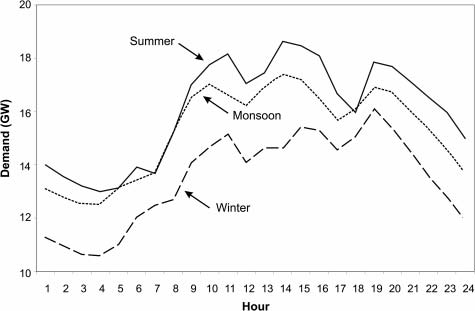
\includegraphics[width=.9\linewidth]{./pictures/daily-e-demand-thailand.png}
\caption{ความผันแปรของอุปสงค์กำลังไฟฟ้าเฉลี่ยใน 1 วันในฤดูร้อน ฤดูฝนและฤดูหนาว \citeprocitem{5}{[5]}}
\end{figure}

ดังนั้น การจะลดผลกระทบจากความผันผวนของอุปสงค์และอุปทานจากแหล่งพลังงานทดแทนเช่นพลังงานแสงอาทิตย์หรือพลังงานลม จำเป็นที่จะต้องมีอุปกรณ์กับเก็บพลังงานที่มีประสิทธิภาพเพื่อเก็บพลังงานส่วนเกินไว้ แล้วสามารถดึงพลังงานที่กเก็บไว้มาใช้ในช่วงที่มีความต้องการได้โดยไม่ต้องพึ่งพาแหล่งพลังงานโดยตรง

วิธีการกับเก็บพลังงานจากแสงอาทิตย์สามารถแบ่งได้เป็นหลายประเภท
ซึ่งแต่ละประเภทก็มีจุดเด่นและจุดด้อยต่างกันไป
พึงคำนึงไว้เสมอว่าไม่มีเทคโนโลยีใดที่ดีกว่าเทคโนโลยีอื่นในทุกสถานการณ์
เราจึงควรทำความเข้าใจประเด็นต่างๆที่สำคัญเหล่านี้ไว้
เพื่อจะได้นำเทคโนโลยีเหล่านี้ไปประยุกต์ใช้ในสถานการณ์ต่างๆได้อย่างเหมาะสม

\section{บ่อกักเก็บพลังงานแสงอาทิตย์}
\label{sec:org4e26301}

บ่อกักเก็บพลังงานแสงอาทิตย์ในที่นี้หมายถึงบ่อกับเก็บของเหลวซึ่งสามารถกับเก็บความร้อนจากพลังงานแสงอาทิตย์เพื่อนำไปใช้ประโยชน์ต่อไปได้ ในปัจจุบันบ่อกักเก็บพลังงานแสงอาทิตย์ส่วนมากใช้สารละลายเกลือคลอไรด์หรือซัลเฟตในน้ำ หลักการทำงานของบ่อดังกล่าวคือการแบ่งชั้นของสารละลายตามความความเข้มข้น โดยสารละลายที่มีความเข้มข้นมากจะตกอยู่ที่ชั้นล่างเนื่องจากมีความหนาแน่นสูง และสารละลายที่มีความเข้มข้นน้อยจะลอยอยู่ด้านบนเนื่องจากมีความหนาแน่นน้อย ซึ่งการแบ่งชั้นนี้จะป้องกันการหมุนเวียนของสารละลายเมื่อได้รับความร้อน ซึ่งในบ่อน้ำปกติเมื่อได้รับความร้อน จะมีการหมุนเวียนขึ้นเนื่องจากน้ำที่ร้อนกว่าจะมีการขยายตัว ทำให้ความหนาแน่นลดลงและลอยขึ้นสู่ด้านบน แต่ในบ่อน้ำที่มีการแบ่งชั้นของสานละลายนี้จะไม่มีการหมุนเวียนของสารละลาย ทำให้สามารถกักเก็บความร้อนไว้ได้

กระบวนการสร้างบ่อกักเก็บพลังงานแสงอาทิตย์มีอยู่ 2 วิธี

\section{บ่อกักเก็บแบบประดิษฐ์}
\label{sec:org040bb57}
บ่อกักเก็บพลังงานแบบนี้สร้างโดยการเติมสารละลายที่มีความเข้มข้นจากสูงลงไปสู่ชั้นล่างแล้วลดลงต่ำลงเมื่อเพิ่มระดับน้ำขึ้นเรื่อยๆ
จนเมื่อเติมเสร็จ บ่อก็จะสามารถกับเก็บพลังงานแสงอาทิตย์ไว้ได้

\section{บ่อกักเก็บแบบเกิดเอง}
\label{sec:orgf047f51}
บ่อประเภทนี้อาศัยหลักการของการละลายอิ่มตัวของเกลือในน้ำที่อุณหภูมิต่างๆกัน
โดยที่ความสามารถในการละลายแปรผันตรงกับอุณหภูมิของตัวทำละลาย
ซึ่งเกลือที่จะนำมาใช้ในบ่อประเภทนี้
จำเป็นจะต้องมีอัตราการเปลี่่ยนแปลงความสามารถในการละลายต่ออุณหภูมิสูง
เพื่อที่จะได้สามารถสร้าง gradient ของความเค็มต่อความลึกได้สูง
และมีความสามารถในการเก็บความร้อนได้ดี

\section{แบตเตอรี่}
\label{sec:org7b2c92d}

แบตเตอรี่ที่เราจะพูดถึงในบทนี้เป็นแบตเตอรี่ทุติยภูมิ หรือแบตเตอรี่ที่ประจุไฟใหม่ได้ (rechargeable batteries หรือ secondary cell) เพื่อนำมาใช้ในเป็นตัวกลางกักเก็บพลังงานจากการผลิตไฟฟ้าของพลังงานหมุนเวียนชนิดอื่น โดยแบตเตอรี่แบบเติมประจุได้นี้มีหลายชนิด เช่น

\begin{itemize}
\item แบตเตอรี่แบบตะกั่ว-กรด (lead-acid battery)
\item แบตเตอรี่นิเกิล-แคดเมียม (NiCd)
\item แบตเตอรี่นิเกิลเมตทัลไฮไดรด์ (nickel-metal hydride, NiMH)
\item แบตเตอรี่ลิเทียม-ไอออน (lithium-ion, Li-Ion)
\item แบตเตอรี่ลีเทียม-ไอออน พอลิเมอร์ (lithium-ion polymer, LiPo)
\end{itemize}

สาเหตุที่แบตเตอรี่แบบนี้สามารถเติมประจุได้เพราะใช้ปฏิกิริยาไฟฟ้าเคมีที่สามารถย้อนกลับได้ (reversible electrochemical reaction)

\subsection{{\bfseries\sffamily TODO} การชาร์จและการคายประจุ}
\label{sec:org29080b4}

ในระหว่างการเติมประจุ วัสดุที่เป็นขั้วบวกจะถูกออกซิไดซ์และให้อิเลกตรอน ส่วนวัสดุที่เป็นขั้วลบจะถูกรีดิวซ์และรับอิเลกตรอน อิเลกตรอนที่เกิดจากปฏิกิริยานี้ทำให้เกิดการไหลของกระแสเมื่อต่อให้ครบวงจร สำหรับอิเลกโทรไลต์ที่อยู่ในแบตเตอรี่อาจเป็นได้ทั้งตัวนำกระแสระหว่างขั้ว (อย่างเช่นในกรณีของแบตเตอรี่ลิเทียม-ไออน) หรืออาจะเป็นหนึ่งในสารตั้งต้นที่ทำให้เกิดปฏิกิริยารีดอกซ์ขึ้น (เช่นกรณีของแบตเตอรี่ตะกั่ว-กรด)

\subsection{{\bfseries\sffamily TODO} แบตเตอรี่ตะกั่ว-กรด}
\label{sec:orga3f0368}

\begin{marginfigure}
  \centering
  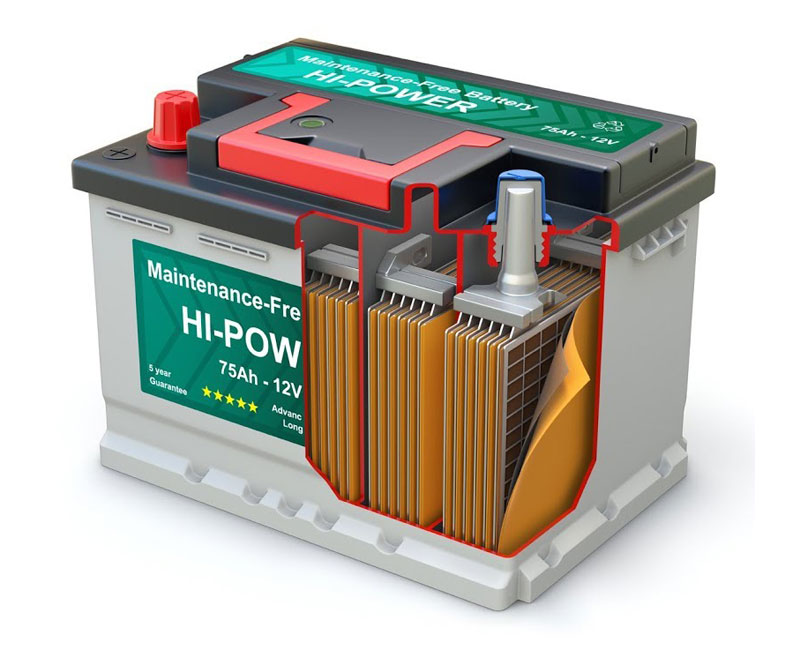
\includegraphics[width=\textwidth]{pictures/lead-acid-battery}
\caption{แบตเตอรี่ตะกั่ว-กรด}
\end{marginfigure}

ปฏิกิริยาที่ขั้วลบ:

$$ \ce{Pb + HSO4^-(aq) <=> PbSO4(s) + H^+(aq) + 2e^-} $$

ปฏิกิริยาที่ขั้วบวก:

$$ \ce{PbO2(s) + HSO4^-(aq) + 3H^+(aq) + 2e^- <=> PbSO4(s) + 2H2O(l)} $$

ข้อดีของแบตเตอรี่ชนิดนี้คือเนื่องจากเป็นเทคโนโลยีเก่าและมีใช้อย่างแพร่หลายในรถยนต์ จึงทำให้มีราคาถูกมาก นอกจากนี้ยังสามารถส่งกระแสไฟกระชากได้ดี แต่เนื่องจากมีขนาดใหญ่และประสิทธิภาพต่ำกว่าแบตเตอรี่อื่นๆ จึงทำให้เหมาะกับการใช้เป็นอุปกรณ์เก็บพลังงานขนาดใหญ่มากกว่าสำหรับใช้ในอุปกรณ์พกพา

ตัวแบตเตอรี่เองมีปัญหา

\begin{enumerate}
\item การเกิดชั้นของกำมะถันขึ้นที่ขั้วซึ่งกันกระแสไฟฟ้าไหลผ่าน
\item การแยกชั้นของน้ำกับกรดซัลฟิวริก ทำให้ไม่เกิดปฏิกิริยา
\item ในบางกรณี \(\ce{H2}\) และ \(\ce{O2}\) อาจค้างอยู่ด้านในของแบตเตอรี่ทำให้เกิดการระเบิดขึ้น
\end{enumerate}

\subsection{{\bfseries\sffamily TODO} แบตเตอรี่นิเกิล-แคดเมียม}
\label{sec:org53c73c2}

\begin{marginfigure}
  \centering
  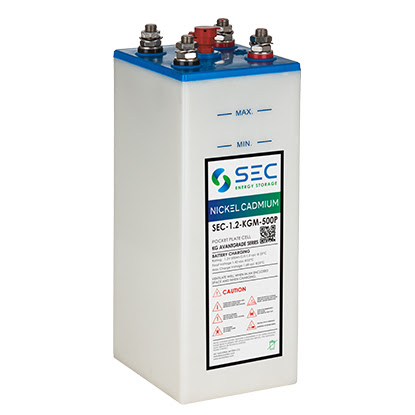
\includegraphics[width=\textwidth]{pictures/nickel-cadmium-battery}
\caption{แบตเตอรี่นิเกิล-แคดเมียม}
\end{marginfigure}

แคดเมียม (ขั้วบวก)
$$ \ce{Cd + 2OH^- <=> Cd(OH)_2 + 2e^-} $$

นิเกิลออกไซด์ไฮดรอกไซด์ (ขั้วลบ)
$$ \ce{2NiO(OH) + 2H_2O + 2e^- <=> 2Ni(OH)_2 + 2OH^-} $$

สำหรับข้อดีของแบตเตอรี่ชนิดนี้คือ สามารถเติมประจุใหม่ได้หลายครั้ง ทำงานได้ดีที่อุณหภูมิต่ำ อัตราการจ่ายกระแสไม่มีผลกระทบกับความจุประจุ ส่วนข้อเสียคือแคดเมียมเป็นโลหะหนักที่เป็นพิษอย่างร้ายแรง นอกจากนี้ยังมีปัญหาเรื่อง \textbf{ความจำ} การเติมประจุ และเนื่องจากมีราคาแพงกว่าแต่มีความจุน้อยกว่าแบตเตอรี่แบบนิกเกิลเมตทัลไฮไดรด์ ปัจจุบันจึงไม่มีการใช้แบตเตอรี่ชนิดนี้แล้ว

\subsection{{\bfseries\sffamily TODO} แบตเตอรี่นิเกิลเมตทัลไฮไดรด์}
\label{sec:orgd66c505}

\begin{marginfigure}
  \centering
  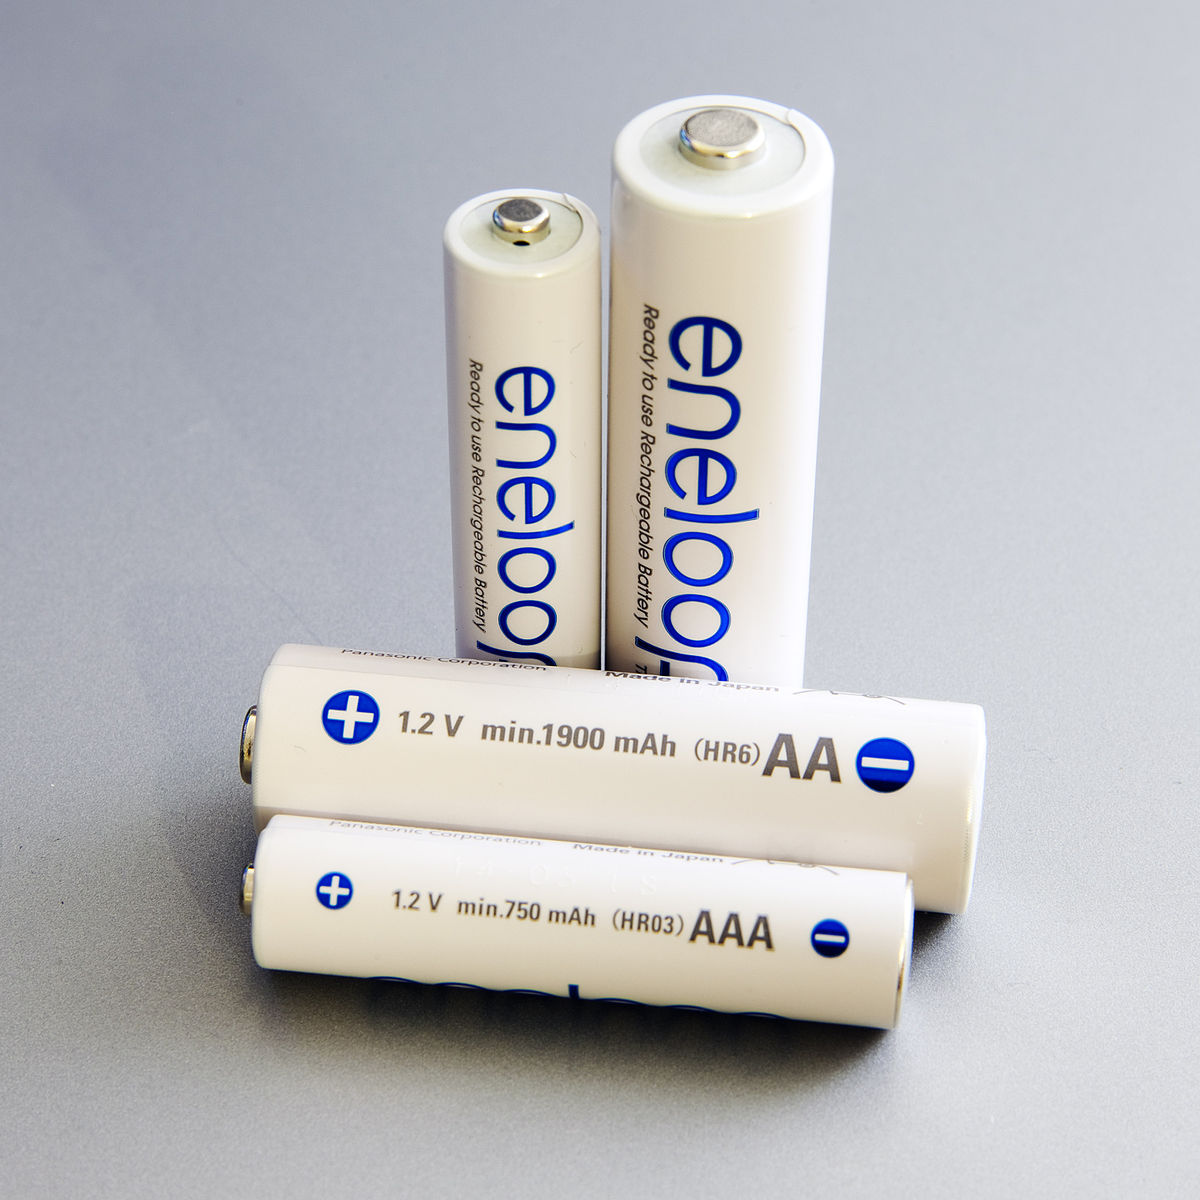
\includegraphics[width=\textwidth]{pictures/nimh-battery}
\caption{แบตเตอรี่นิเกิลเมตทัลไฮไดรด์}
\end{marginfigure}

ขั้วลบ:
$$ \ce{H2O + M + e^- <=> OH^- + MH} $$

ขั้วบวก:
$$ \ce{Ni(OH)2 + OH^- <=> NiO(OH) + H2O + e^-} $$

ข้อดีของแบตเตอรี่ชนิดนี้คือมีความจุเพิ่มขึ้นเป็น 2-3 เท่าของแบตเตอรี่ NiCd ขนาดเดียวกัน และไม่ต้องพึ่งพาแคดเมียม นอกจากนี้ยังลดปัญหาเรื่องความจำลงไปได้เยอะ จึงได้ถูกนำมาใช้อย่างแพร่หลายในอุปกรณ์อิเลกทรอนิกส์ทั่วไปและในรถยนต์ไฟฟ้า

\subsection{{\bfseries\sffamily TODO} แบตเตอรี่ลิเทียมไอออน}
\label{sec:orgf65e1ea}

\begin{marginfigure}
  \centering
  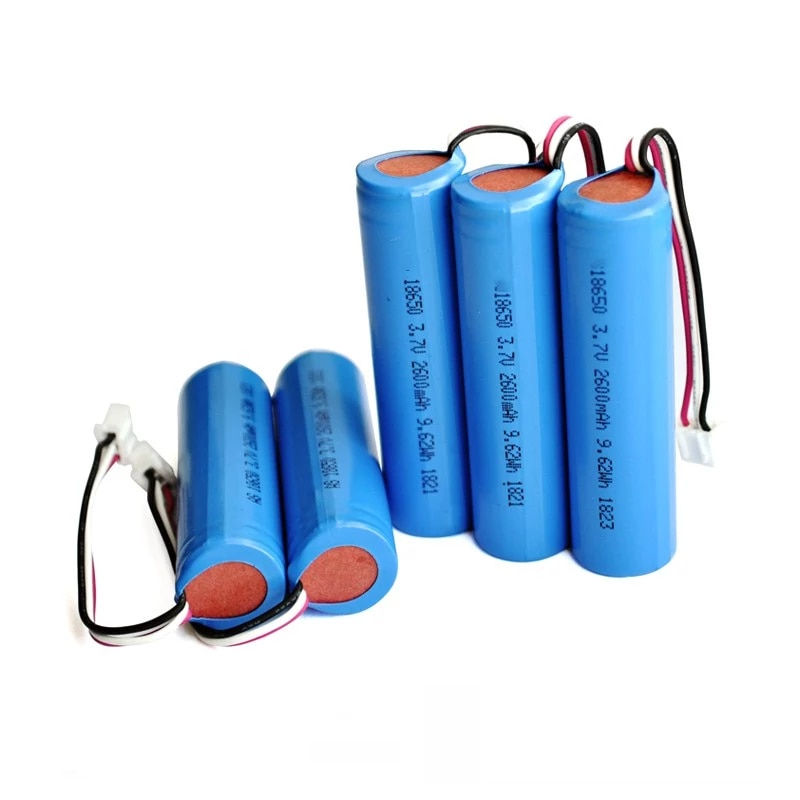
\includegraphics[width=\textwidth]{pictures/liion-battery}
\caption{แบตเตอรี่ลิเทียมไออน}
\end{marginfigure}

Negative:
$$ \ce{LiC6 <=> C6 + Li^+ + e^-} $$

Positive:
$$ \ce{CoO2 + Li^+ + e^- <=> LiCoO2} $$

แบตเตอรี่ชนิดนี้มีข้อดีหลายประการ เช่น มีความจุไฟฟ้าสูง น้ำหนักเบา แทบจะไม่มีปัญหาเรื่องความจำ มีอัตราการสูญเสียประจุระหว่างไม่ใช้งานต่ำ แต่ข้อที่พึงพิจารณานอกจากเรื่องราคาที่สูงก็จะเป็นเรื่องของอุณหภูมิในช่วงการใช้งานและช่วงการประจุไฟ ซึ่งหากสูงเกินไปจะทำให้อายุการใช้งานสั้นลงหรือแม้แต่เกิดผลข้างเคียงเช่นแก๊สที่ติดไฟ ทำให้เกิดการระเบิดได้

ส่วนประกอบสำคัญของแบตเตอรี่ลิเทียมไออนคือ

\begin{itemize}
\item ขั้วลบ มีองค์ประกอบหลักเป็นคาร์บอนที่มีรูพรุน (เช่น แกรไฟต์) เคลือบบนแผ่นทองแดง
\item ขั้วบวกเป็นลิเทียมเมทัลออกไซด์เคลือบบนแผ่นอะลูมิเนียม
\item สารละลายอิเล็กโทรไลต์ ประกอบด้วยเกลือของลิเทียม เช่น \(\ce{LiPF6}\) หรือ \(\ce{LiBF4}\) ในตัวทำละลาย เช่น เอทิลีนคาร์บอเนต (ethylene carbonate) ไดเอทิลคาร์บอเนต (diethyl carbonate) และ/หรือ ไดเมทิลคาร์บอเนต (dimethyl carbonate)
\item เยื่อเลือกผ่าน (separator) กั้นระหว่างขั้วทั้งสอง ทำจากพอลิโพรพิลีน (polypropylene, PP) และ/หรือพอลิเอทิลีน (polyethylene, PE)
\end{itemize}

\subsection{{\bfseries\sffamily TODO} เปรียบเทียบแบตเตอรี่}
\label{sec:org10c49be}

\begin{figure}[htbp]
\centering

\includegraphics[width=.9\linewidth]{./pictures/battery-energy-density-comparison.png}
\caption{\label{fig:orgd672c5e}แผนภูมิเปรียบเทียบพลังงานจำเพาะและความหนาแน่นพลังงานของแบตเตอรี่ทุติยภูมิ}
\end{figure}

\section{ล้อตุนกำลัง}
\label{sec:orgda5756f}

ล้อตุนกำลังเป็นระบบที่เก็บพลังงานที่ต้องการในรูปของพลังงานจลน์จากการหมุนของล้อตุนกำลังด้วยความเร็วสูง เมื่อต้องการนำพลังงานที่เก็บออกมาใช้ก็จะทำให้ความเร็วของล้อตุนกำลังลดลง และเมื่อเติมพลังงานให้ ล้อก็จะหมุนเร็วขึ้น โดยมากแล้วระบบล้อตุนกำลังจะใช้ไฟฟ้าในการเร่งและหน่วงระบบ แต่ระบบที่ใช้พลังงานกลโดยตรงกำลังได้รับการพัฒนาอยู่เช่นกัน

\section{ส่วนประกอบของระบบล้อตุนกำลัง}
\label{sec:org40b85fa}

\begin{figure}[htbp]
\centering
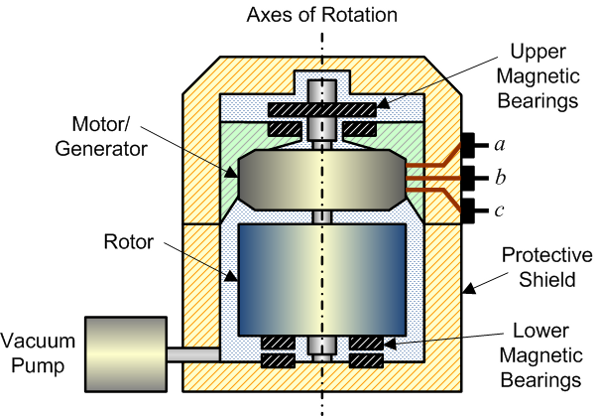
\includegraphics[width=.9\linewidth]{./pictures/flywheel-components.png}
\caption{ระบบล้อตุนกำลังแบบใช้แบร์ริงแม่เหล็ก}
\end{figure}

\begin{enumerate}
\item มอเตอร์ -
เครื่องปั่นไฟฟ้าเพื่อใช้ในการแปลงพลังงานจลน์ไปเป็นพลังงานไฟฟ้าและจากพลังงานไฟฟ้าเป็นพลังงานจลน์

\item แบร์ริง
ซึ่งเป็นส่วนหลักที่ทำให้มีการสูญเสียพลังงานเนื่องจากความเสียดทานจากแบร์ริงแบบตลับลูกปืนทั่วไป
อย่างไรก็ดี
ในระบบล้อตุนกำลังแบบใหม่มักใช้แบร์ริงแบบแม่เหล็กไฟฟ้าเพื่อลดการสูญเสียพลังงานส่วนนี้

\item ในบางกรณี
อาจจะมีระบบปั๊มสุญญากาศเพื่อลดการสูญเสียพลังงานจากแรงเสียดทานอากาศด้วย
\end{enumerate}

\section{พลังงานที่สะสมในล้อตุนกำลัง}
\label{sec:org4648338}
พลังงานจลน์ที่สะสมในล้อตุนกำลังสามารถหาได้จากสมการ
\[E = \frac{1}{2}J \omega^2\] โดยที่ \(J\)
คือโมเมนต์ความเฉื่อยเชิงมุมของล้อ และ \(\omega\)
คือความเร็วเชิงมุมของล้อ อย่างไรก็ตาม
ล้อตุนกำลังเองก็มีข้อจำกัดที่ไม่สามารถจะหมุนเร็วเกินไปได้
เนื่องจากเมื่อความเร็วเชิงมุมสูงก็จะมีความเค้นตามเส้นรอบรูป (hoop
stress) สูงขึ้นด้วยเช่นกัน

\section{วัสดุสำหรับล้อตุนกำลัง}
\label{sec:orgdb5f9e5}
หากจะพิจารณาหาวัสดุที่เหมาะจะนำมาสร้างล้อตุนกำลัง
จำเป็นจะต้องพิจารณาถึงพลังงานจำเพาะ (พลังงานต่อมวล)
ที่วัสดุสามารถเก็บได้ ซึ่งสามารถคำนวณได้จาก
\[\frac{E}{J} = K \left( \frac{S_{ut}}{\rho} \right)\] โดยที่ \(K\) เป็น
shape factor ของล้อตุนกำลัง \(S_{ut}\) เป็นค่าความต้านทานแรงดึงสูงสุด
(ultimate tensile strength) และ \(\rho\) คือความหนาแน่นของวัสดุ
จะเห็นได้ว่าค่าพลังงานจำเพาะนั้นขึ้นอยู่กับรูปร่างของล้อและอัตราส่วนความแข็งแรงต่อมวลของวัสดุล้อ

ค่า shape factor ของรูปทรงเรชาคณิตต่างๆมีดังนี้

\begin{figure}[htbp]
\centering
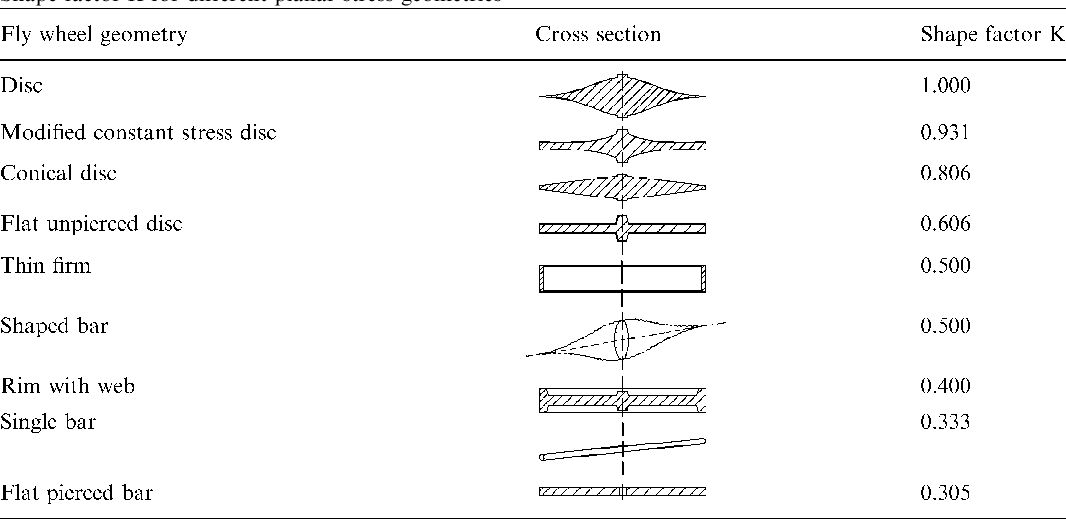
\includegraphics[width=.9\linewidth]{./pictures/flywheel-shape-factor.png}
\caption{ค่า shape factor ของภาคตัดรูปทรงต่างๆที่ใช้ทำล้อตุนกำลัง}
\end{figure}

สำหรับค่าอัคราส่วนความแข็งแรงต่อมวลของวัสดุต่างๆมีดังนี้

\begin{table}[htbp]
\caption{อัตราส่วนความแข็งแรงต่อมวลของวัสดุสำหรับผลิตล้อตุนกำลัง}
\centering
\begin{tabular}{p{2.5cm}p{3cm}p{3.5cm}}
\toprule
Material & Specific tensile strength (kJ/kg) & Remarks\\[0pt]
\midrule
Ceramics & 200 - 2000 & Brittle and weak in tension\\[0pt]
CFRP & 200 - 500 & Best performance\\[0pt]
GFRP & 100 - 400 & Almost as good, but cheaper\\[0pt]
Beryllium & 300 & Best metal, but expensive and toxic\\[0pt]
High strength steel & 100 - 200 & Cheaper than Mg and Ti\\[0pt]
High strength Al & 100 - 200 & Cheaper than Mg and Ti\\[0pt]
High strength Mg & 100 - 200 & Equal performance to steel and Al\\[0pt]
Ti Alloys & 100 - 200 & Equal performance to steel and Al\\[0pt]
Lead alloy & 3 & Poor performance\\[0pt]
Cast iron & 8 - 10 & Poor performance\\[0pt]
\bottomrule
\end{tabular}
\end{table}

\subsection{การออกแบบล้อตุนกำลังสำหรับรถโดยสารประจำทาง}
\label{sec:org7200c82}

เราต้องการจะออกแบบล้อตุนกำลังสำหรับรถประจำทางเพื่อใช้ในการชาร์จไฟระหว่างจอดรับผู้โดยสาร
และขับเคลื่อนรถในช่วงออกตัว เพื่อให้รับพลังงานได้ 50 kJ มีวัสดุให้เลือก
4 วัสดุซึ่งมีคุณสมบัติดังต่อไปนี้

\begin{table}[htbp]
\caption{คุณสมบัติของวัสดุสำหรับออกแบบล้อตุนกำลัง}
\centering
\begin{tabular}{lrp{3cm}}
\toprule
Material & Density (kg/m\(^{\text{3}}\)) & Ultimate Tensile Strength (MPa)\\[0pt]
\midrule
CFRP & 1500 & 550\\[0pt]
High strength steel & 7800 & 1500\\[0pt]
Cast Iron & 7300 & 200\\[0pt]
\bottomrule
\end{tabular}
\end{table}

การออกแบบล้อตุนกำลังสามารถทำได้โดยใช้สมการคำนวณพลังงานจลน์และความเค้นดังนี้
\begin{gather*}
  E = \frac{1}{2} J \omega^2 \\
  J = \frac{1}{2} m r^2 \\
  \sigma_t = \rho r^2 \omega^2
\end{gather*}
ซึ่งจากการวิเคราะห์สมการ
หากเรากำหนดให้ล้อตุนกำลังจากทุกวัสดุใช้ความหนา \(t\) เท่ากัน
เราจะสามารถคำนวณรัศมีและมวลของล้อได้ดังนี้

\begin{gather*}
  E = \frac{1}{4} m r^2 \omega^2 \\
  r^2 \omega^2 = \frac{\sigma_t}{\rho} \\
  E = \frac{1}{4} m \frac{\sigma_t}{\rho} \\
  m = \rho \pi r^2 t \\
  r = \sqrt{ \frac{4E}{\pi t \sigma_t}}
\end{gather*}

เมื่อแก้สมการหาค่ารัศมีโดยกำหนดให้ความเค้นมากที่สุดของล้อกำลัง
\(\sigma_t = S_{ut}\) จะได้มวลและรัศมีของล้อตุนกำลังจากวัสดุต่างๆดังนี้

\begin{center}
\begin{tabular}{lrr}
\toprule
Material & Radius (m) & Mass (kg)\\[0pt]
\midrule
CFRP & 0.048 & 0.545\\[0pt]
HSS & 0.029 & 1.040\\[0pt]
Cast Iron & 0.080 & 7.300\\[0pt]
\bottomrule
\end{tabular}
\end{center}

ซึ่งจะเห็นได้ว่า CFRP ให้ล้อตุนกำลังที่มีมวลเบาที่สุด
เนื่องจากอัตราส่วนความแข็งแรงจำเพาะสูงที่สุด
แต่หากมีข้อจำกัดเรื่องของขนาด ล้อที่ทำจาก HSS มีรัศมีน้อยที่สุด

\section{โรงไฟฟ้าพลังน้ำแบบสูบกลับ}
\label{sec:org3a07312}
เป็นหลักการกักเก็บพลังงานโดยแปลงพลังงานชนิดอื่น (มักจะเป็นพลังงานไฟฟ้า)
มาเป็นพลังงานศักย์ในรูปของน้ำเหนือเขื่อน


\epigraph{การจะปฏิรูปเศรษฐกิจ ปกป้องความมั่นคง และรักษาโลกของเราจากเงื้อมมือของการเปลี่ยนแปลงสภาพภูมิอากาศนั้น สิ่งที่จำเป็นที่สุดคือเราจะต้องทำให้พลังงานทดแทนที่สะอาดกลายเป็นพลังงานที่สร้างกำไรได้}{บารัค โอบามา}

เคยสงสัยกันบ้างไหมว่า เวลาที่การไฟฟ้าเก็บค่าไฟเราหน่วยละ 3 บาทกว่าๆนั้น
เขาคิดคำนวณกันมาอย่างไร
มีหลักฐานอ้างอิงหรือข้อมูลอะไรมาช่วยสนับสนุนนี้ไหม
หรือว่าแค่นั่งเทียนกำหนดเลขกลมๆขึ้นมา จริงๆแล้วก็คงไม่ใช่อย่างนั้น
และแน่นอนว่าค่าไฟที่เก็บนั้นก็คงไม่ได้เท่าทุนพอดี
คงจะต้องมีส่วนบวกเพื่อให้เป็นกำไรไว้ไม่มากก็น้อยเป็นแน่

ในบทนี้ เราจะมาพูดถึงการวิเคราะห์ต้นทุนทางเศรษฐศาสตร์ของการผลิตพลังงานเพื่อใช้ในการเปรียบเทียบระหว่างการผลิตไฟฟ้าปัจจุบัน (พ.ศ. 2560) โดยส่วนมากยังพึ่งพาเชื้อเพลิงปิโตรเลียมอยู่กับการผลิตไฟฟ้าจากพลังงานทดแทนซึ่งเราได้กล่าวถึงเทคโนโลโยีและอุปกรณ์ที่ต้องใช้ไปในส่วนที่ 1

หลายครั้งที่วิศวกรโดยเฉพาะอย่างยิ่งในสถานศึกษา (ตัวผมเองก็ด้วย) คิดวิเคราะห์ปัญหาทางพลังงานที่มีอยู่ในปัจจุบันโดยยังไม่ได้พิจารณาเรื่องของความเหมาะสมของเทคโนโลยีทางเศรษฐศาสตร์ หรือที่เรียกง่ายๆว่า เทคโนโลยีนั้นมันแพงเกินไปหรือเปล่า การจะพิจารณาความเป็นไปได้ที่จะนำเทคโนโลยีพลังงานหนึ่งๆมาใช้ แม้ว่าจะมีความล้ำสมัย สะอาด และเป็นมิตรต่อสิ่งแวดล้อมเพียงใด หากมีราคาแพงกว่าของเดิมที่ใช้อยู่ปัจจุบัน ก็ยากที่จะโน้มน้าวให้ประชาชนส่วนมากเห็นดีเห็นงามไปด้วย ไม่ใช่ว่าพวกเขาไม่ได้รักโลก หรือไม่ห่วงเรื่องสิ่งแวดล้อม แต่ว่าการจะบอกว่าได้โปรดใช้ของที่แพงขึ้นหน่อยเพื่อให้โลกสะอาดขึ้นก็ฟังดูเป็นข้ออ้างที่อาจจะดูหลักลอยไปสักหน่อย วิธีง่ายที่สุดที่จะชวนให้ประชาชนทั่วไปหันมาสนใจการใช้พลังงานทดแทนอย่างจริงจังก็คือต้องบอกว่าของใหม่นั้น*ถูกกว่า*

ดังนั้น เพื่อจะแน่ใจว่าเทคโนโลยีพลังงานทดแทนของเรานั้นถูกกว่าไฟฟ้าที่ผลิตอยู่ปัจจุบัน เราจำเป็นจะต้องทำความเข้าใจก่อนว่าโครงสร้างต้นทุนการผลิตไฟฟ้า หรือพลังงานอื่นๆที่ใช้ในครัวเรือนปัจจุบันนั้นเป็นอย่างไร

\chapter{เศรษฐศาสตร์วิศวกรรมเบื้องต้น}
\label{sec:orgdf905e0}

\epigraph{เงินมักจะราคาแพงเกินไปอยู่เสมอ}{Ralph Waldo Emerson}

\section{มูลค่าเงินตามเวลา (Time Value of Money)}
\label{sec:orge2a41af}
แนวคิดเรื่องของมูลค่าเงินตามเวลานั้นว่าด้วยมูลค่าของเงินที่เปลี่ยนแปลงไป
ขึ้นอยู่กับเวลาที่เราได้รับหรือจ่ายเงินนั้นออกไป
ฟังดูอาจจะแปลกๆอยู่สักหน่อย 100 บาทวันนี้ พรุ่งนี้ก็ยัง 100
บาทอยู่มิใช่หรือ แต่หากเริ่มเพิ่มเวลาเข้าไปเป็น 1 เดือน 1 ปี 10 ปี
เงินนี้ก็อาจจะไม่เหมือนเดิมแล้ว พิจารณาได้อย่างง่ายด้วยคำถามนี้
หากมีคนสัญญาว่าจะให้เงินเรา 100 บาทตอนนี้เลยหรือ 100 บาทในอีก 10
ปีข้างหน้า ทุกคนคงตอบพร้อมเป็นเสียงเดียวกันว่า ขอเงิน 100
บาทตอนนี้เลยก็แล้วกัน นั่นเป็นเพราะว่าเงิน 100
บาทตอนนี้มี \textbf{มูลค่า} มากกว่าเงิน 100 บาทในอีก 10 ปีข้างหน้า

\section{ต้นทุนเฉลี่ยตลอดอายุโครงการ (Levelized Cost)}
\label{sec:org6e432d2}
ในมุมมองของหน่วยงานควบคุมราคาหรือคุ้มครองผู้บริโภค ความสามารถในการทำกำไรหรืออัตราผลตอบแทนของโครงการโรงงานผลิตไฟฟ้าหนึ่งมักจะไม่ใช่สิ่งแรกที่น่าสนใจ ราคาต่อหน่วยพลังงานที่ผู้บริโภคจะต้องจ่ายเป็นตัววัดที่สามารถนำมาช่วยพิจารณาความเหมาะสมของการเลือกใช้พลังงานทางเลือกเพื่อผลิตไฟฟ้า

\begin{align*}
\label{eq:orgbb923b9}
  \text{LCOE} &= \frac{\text{ผลรวมของต้นทุนที่พิจารณามูลค่าเงินตามเวลา}}{\text{ผลรวมของพลังงานไฟฟ้าที่ผลิตได้}} \\[10pt]
 &= \dfrac{\sum \dfrac{I_t + M_t + F_t}{(1+r)^t}}{\sum E_t} \\[10pt]
              &= \frac{\text{มูลค่าปัจจุบันสุทธิของต้นทุน}}{\text{พลังงานไฟฟ้าที่ผลิตได้ทั้งหมด}}
\end{align*}

\section{การวิเคราะห์ความเป็นไปได้ทางเศรษฐศาสตร์}
\label{sec:org5924c2c}
\section{อัตราผลตอบแทนภายใน (Internal Rate of Return - IRR)}
\label{sec:org39f69bd}
การจะวิเคราะห์

\section{มูลค่าปัจจุบันสุทธิ (Net Present Value - NPV)}
\label{sec:org543ad0e}

\section{โครงสร้างต้นทุน}
\label{sec:org9edacf4}
ศาสตร์เรื่องการวิเคราะห์โครงสร้างต้นทุนนั้นมีมานานโขอยู่ เริ่มจากปี \ldots{}
ซึ่งพลังงานก็นับเป็นผลิตภัณฑ์อย่างหนึ่งซึ่งใช้สามารถจะวิเคราะห์ต้นทุนได้
การแบ่งประเภทต้นทุนนั้นสามารถทำได้อยู่หลายวิธี
แล้วแต่จุดประสงค์และการนำไปใช้ประโยชน์ อย่างไรก็ดี
ในหนังสือเล่มนี้เราต้องการศึกษาประเภทของต้นทุนเพื่อทำความเข้าใจแนวโน้มการเปลี่ยนแปลงเมื่อมีการพัฒนาเทคโนโลยีต่างๆที่เปลี่ยนไป
จึงได้เลือกใช้วิธีการจำแนกต้นทุนตามความสัมพันธ์กับระดับของกิจกรรม
ซึ่งสามารถสะท้อนความเปลี่ยนแปลงอันขึ้นอยู่กับระดับการผลิต
โดยโครงสร้างต้นทุนแบบนี้สามารถแบ่งออกเป็นประเภทดังนี้

\section{ต้นทุนคงที่ (Fixed Costs)}
\label{sec:orgb73c8de}
เป็นต้นทุนส่วนที่ไม่มีการเปลี่ยนแปลงในช่วงระดับการผลิตหนึ่ง
ซึ่งทำให้ต้นทุนต่อหน่วยลดลงเมื่อเพิ่มปริมาณการผลิตมากขึ้น

\section{ต้นทุนผันแปร (Variable Costs)}
\label{sec:orgca03754}
เป็นต้นทุนส่วนที่ต้นทุนรวมมีการเปลี่ยนแปลงขึ้นอยู่กับปริมาณการผลิต
ในขณะที่ต้นทุนต่อหน่วยยังคงที่

\section{ต้นทุนผสม (Mixed Costs)}
\label{sec:org2668b58}
เป็นต้นทุนที่มีลักษณะของทั้งต้นทุนคงที่และผันแปรผสมกัน
สามารถแบ่งได้เป็นสองประเภท

\begin{enumerate}
\item ต้นทุนกึ่งผันแปร (semi variable cost)
เป็นต้นทุนที่จะมีส่วนหนึ่งคงที่ทุกระดับกิจกรรม
และมีส่วนที่ผันแปรไปกับระดับกิจกรรม เช่น ค่าโทรศัพท์ เป็นต้น
บางครั้งก็เป็นการยากที่จะประเมินส่วนที่คงที่หรือแปรผันของส่วนนี้

\item ต้นทุนเชิงขั้น (step cost) หรือต้นทุนกึ่งคงที่ (semi fixed cost)
หมายถึงต้นทุนที่คงที่ในช่วงระดับกิจกรรมหนึ่ง
และเปลี่ยนไปคงที่ในอีกระดับกิจกรรมหนึ่ง เช่น ค่าผู้ควบคุมงาน
เงินเดือน
\end{enumerate}

\section{ต้นทุนของพลังงานจากเทอร์โมอิเลกทริก}
\label{sec:orged105ef}

\begin{table}[htbp]
\caption{ต้นทุนวัสดุที่ใช้ทำเทอร์โมอิเลกทริกในปัจจุบัน}
\centering
\begin{tabular}{lrrlp{1cm}}
\toprule
Material Family & Max \(ZT\) & Temp (°C) & Efficiency & Material Cost (\$/kg)\\[0pt]
\midrule
Cobalt Oxide & 1.4 & 727 & 12\% & 345\\[0pt]
Cobalt Oxide & 1.4 & 727 & 12\% & 345\\[0pt]
Clathrate & 1.4 & 727 & 12\% & 5,310\\[0pt]
SiGe & 0.86 & 727 & 9\% & 6,033\\[0pt]
Chalcogenide & 2.27 & 727 & 16\% & 730\\[0pt]
Half-Heusler & 1.42 & 427 & 17\% & 1,988\\[0pt]
Skutterudite & 1.5 & 427 & 18\% & 562\\[0pt]
Silicide & 0.93 & 727 & 9\% & 151\\[0pt]
\bottomrule
\end{tabular}
\end{table}

เมื่อทำการวิเคราะห์ด้วยราคาต้นทุนไฟฟ้าที่ผลิตจากเทอร์โมอิเลกทริกด้วยราคาปัจจุบัน (พ.ศ. 2561) จะเห็นได้ว่า ต้นทุนหลักมาจากค่าอุปกรณ์เทอร์โมอิเลกทริก เนื่องจากยังมีราคาสูงและประสิทธิภาพต่ำ

การเปรียบเทียบต้นทุนการผลิตไฟฟ้าจากเทอร์โมอิเลกทริกด้วยอุณหภูมิขนาดกลาง

กรณีเปรียบเทียบ 3 แบบ: น้ำมันเตาเป็นเชื้อเพลิง ความร้อนเหลือทิ้งจากอุตสาหกรรม หรือซื้อไฟฟ้าจากการไฟฟ้าฯ

สมมติฐานที่ใช้ในการวิเคราะห์

\begin{enumerate}
\item การผลิตไฟฟ้าขนาด 1 MW โดยสิ่งก่อสร้างและอุปกรณ์ทั้งหมดมีอายุการใช้งาน
10 ปี

\item ต้นทุนคงที่จากอุปกรณ์เทอร์โมอิเลกทริก อินเวอร์เตอร์ ค่าที่ดิน
และค่าติดตั้ง

\item ต้นทุนแปรผันนับจากค่าซ่อมแซมและค่าเชื้อเพลิง(ถ้ามี)

\item ค่าอินเวอร์เตอร์ 22 บาทต่อวัตต์ ค่าเทอร์โทอิเลกทริกอุณหภูมิสูง 175
บาทต่อวัตต์ ค่าเทอร์โมอิเลกทริกอุณหภูมิกลาง 525 บาทต่อวัตต์

\item ค่าติดตั้ง 10\% ของค่าอุปกรณ์ (TEG + Inverter)

\item ค่าซ่อมแซม 1\% ของค่าอุปกรณ์ต่อปี

\item ไฟฟ้าจากการไฟฟ้าหน่วยละ 4.5 บาท (4.5 บาท / kWh)
\end{enumerate}

ก่อนอื่น เราสามารถคำนวณค่าอุปกรณ์ที่ต้องใช้ในการแปลงไฟฟ้า
ซึ่งประกอบด้วยค่า TEG และ inverter

เปรียบเทียบต้นทุนระหว่างกรณีที่ 1, 2, และ 3 ได้เป็นตารางดังนี้

\begin{center}
\begin{tabular}{lrr}
\toprule
Costs (million THB) & Fuel & Waste\\[0pt]
\midrule
TEGs & 175 & 525\\[0pt]
Inverters & 22 & 22\\[0pt]
Land & 1 & 1\\[0pt]
Installation & 20 & 55\\[0pt]
Maintenance (per year) & 2 & 5.5\\[0pt]
Fuel (per year) & 191 & 0\\[0pt]
\bottomrule
\end{tabular}
\end{center}


และยังสามารถแสดงกระแสเงินสดเปรียบเทียบระหว่างกรณีได้ดังนี้

\begin{center}
\begin{tabular}{rrrrrr}
\toprule
Year & Base & Fuel & Waste & Base-Fuel & Base-Waste\\[0pt]
\midrule
0 & 0.0 & 218.0 & 603.0 & -218.0 & -603.0\\[0pt]
1 & 39.42 & 193.0 & 5.5 & -153.6 & 33.92\\[0pt]
2 & 39.42 & 193.0 & 5.5 & -153.6 & 33.92\\[0pt]
3 & 39.42 & 193.0 & 5.5 & -153.6 & 33.92\\[0pt]
4 & 39.42 & 193.0 & 5.5 & -153.6 & 33.92\\[0pt]
5 & 39.42 & 193.0 & 5.5 & -153.6 & 33.92\\[0pt]
6 & 39.42 & 193.0 & 5.5 & -153.6 & 33.92\\[0pt]
7 & 39.42 & 193.0 & 5.5 & -153.6 & 33.92\\[0pt]
8 & 39.42 & 193.0 & 5.5 & -153.6 & 33.92\\[0pt]
9 & 39.42 & 193.0 & 5.5 & -153.6 & 33.92\\[0pt]
10 & 39.42 & 193.0 & 5.5 & -153.6 & 33.92\\[0pt]
\bottomrule
\end{tabular}
\end{center}

ในขณะเดียวกัน ค่าไฟฟ้าที่ซื้อจากการไฟฟ้าฯสามารถสมมติว่าเป็นค่าคงที่ในแต่ละปี ซึ่งหากเปรียบเทียบกับการลงทุนในระบบ TEG ทั้งสองแบบแล้ว จะสามารถหาผลต่างของกระแสเงินสดเพื่อจะนำไปใช้หาโครงการที่มีมูลค่าปัจจุบันสุทธิ (NPV) สูงสุดได้ดังนี้

จากผลการวิเคราะห์กระแสเงินสดจะเห็นได้ว่าโครงการสร้างโรงไฟฟ้า TEG ทั้งสองแบบยังมีมูลค่าปัจจุบันสุทธิเป็นลบ หมายความว่าโครงการทั้งสองยังมีผลตอบแทนที่ยังไม่น่าพอใจเมื่อเปรียบเทียบกับใช้กระแสไฟฟ้าจากการไฟฟ้าฯ มาลองพิจารณากันเพิ่มว่า ค่าไฟฟ้าจะต้องเป็นเท่าไหร่จึงจะทำให้การลงทุนในโรงงาน TEG นี้คุ้มค่าได้

จะเห็นได้ว่ามูลค่าสุทธิของโรงไฟฟ้าเพิ่มขึ้นเมื่อค่าไฟจากการไฟฟ้าสูงขึ้น เนื่องจากมีความคุ้มค่าในการสร้างแหล่งผลิตไฟฟ้าทดแทนมากขึ้น และที่จุดตัดศูนย์เป็นค่าไฟที่ทำให้การลงทุนสร้างโรงไฟฟ้าใหม่นี้คุ้มค่ามากกว่าการซื้อไฟฟ้าจากการไฟฟ้าต่อไป สำหรับโรงไฟฟ้า TEG แบบใช้เชื้อเพลิงอยู่ที่ประมาณ 24 บาทต่อกิโลวัตต์-ชั่วโมง ส่วนโรงไฟฟ้า TEG แบบใช้ความร้อนเหลือใช้อยู่ที่ประมาณ 7 บาทต่อกิโลวัตต์-ชั่วโมง

\section{ต้นทุนของพลังงานจากเซลล์เชื้อเพลิง}
\label{sec:orgb51a1f7}

\begin{figure}[h]
  \centering
  \begin{tikzpicture}
    \pgfplotstableread[row sep=\\,col sep=&]{
      Year  & Cost   \\
      2006  & 124    \\
      2007  & 106    \\
      2008  &  81    \\
      2009  &  69    \\
      2010  &  59    \\
      2011  &  57    \\
      2012  &  55    \\
      2013  &  55    \\
      2014  &  55    \\
      2020  &  40    \\
      2050  &  30    \\
    }\mydata

    \centering
    \footnotesize
    \begin{axis}[
      scatter,
      only marks,
      nodes near coords,
      width=\textwidth,
      height=0.5\textwidth,
      bar width=0.5cm,
      axis x line=bottom,
      axis y line=left,
      xlabel={Year},
      xtick=data,
      ytick distance=20,
      symbolic x coords={2006,2007,2008,2009,2010,2011,2012,2013,2014,2020,2050},
      legend style={at={(1,1)},anchor=north east, text=Black},
      ]
      \addplot table[x=Year, y=Cost]{\mydata};
    \end{axis}
  \end{tikzpicture}
\caption{\label{orgdb10963}Historical and projected transportation fuel cell system cost}
\end{figure}

\begin{figure}[h]
  \centering
  \begin{tikzpicture}
    \pgfplotstableread[row sep=\\,col sep=&]{
      Year  & MEA  & Bipolar & BOS & BOP \\
      2007  &  40  &     5   &   6 &  60 \\
      2008  &  34  &     5   &   5 &  45 \\
      2009  &  29  &     5   &   4 &  35 \\
      2010  &  18  &     2   &   3 &  25 \\
      2015  &  12  &     2   &   2 &  18 \\
    }\mydata

    \centering
    \footnotesize
    \begin{axis}[
      ybar stacked,
      % nodes near coords,
      width=\textwidth,
      height=0.5\textwidth,
      bar width=0.5cm,
      xlabel={Year},
      ylabel={\$/kW},
      xtick=data,
      reverse legend,
      ytick distance=20,
      symbolic x coords={2006,2007,2008,2009,2010,2015},
      legend style={at={(1,1)},anchor=north east, text=Black},
      ]
      \addplot table[x=Year, y=MEA]{\mydata};
      \addplot table[x=Year, y=Bipolar]{\mydata};
      \addplot table[x=Year, y=BOS]{\mydata};
      \addplot table[x=Year, y=BOP]{\mydata};
      \legend{MEA, Bipolar, BOS, BOP};
    \end{axis}
  \end{tikzpicture}
\caption{\label{orgc2cdd7c}Historical and projected transportation fuel cell system cost}
\end{figure}

\section{ต้นทุนการผลิตไฟฟ้าพลังงานลม}
\label{sec:org6f7a3e1}
เนื่องจากว่าลมเป็นพลังงานที่ได้เปล่า ต้นทุนในการผลิตส่วนมากจึงมาจากค่าอุปกรณ์กังหัน

\begin{figure}[h]
  \centering
  \begin{tikzpicture}
    \pgfplotstableread[row sep=\\,col sep=&]{
      Cost Item  & Turbine    & BOS    & Financial \\
      Land-based & 1221       & 345    & 154       \\
      Offshore   & 1952       & 2277   & 1084      \\
    }\mydata

    \centering
    \begin{axis}[
      xbar stacked,
      width=0.9\textwidth,
      height=0.5\textwidth,
      bar width=1cm,
      xmin=0,
      xtick distance=1000,
      xlabel={Cost of Components (\$/kW)},
      ytick=data,
      symbolic y coords={Offshore, Land-based},
      % ytick=data,
      legend style={at={(1,1)},anchor=north east, text=Black},
      enlarge y limits=0.5,
      ]
      \addplot table[x=Turbine, y=Cost Item]{\mydata};
      \addplot table[x=BOS, y=Cost Item]{\mydata};
      \addplot table[x=Financial, y=Cost Item]{\mydata};
      \legend{Turbine,BOS,Financial};
    \end{axis}
  \end{tikzpicture}
\end{figure}

\begin{figure}[h]
  \begin{tikzpicture}
    \pgfplotstableread[row sep=\\,col sep=&]{
      Cost Item  & Turbine    & BOS    & Financial & OM       \\
      Land-based & 35         & 10     & 3         & 15       \\
      Offshore   & 51         & 60     & 29        & 39      \\
    }\mydata

    \centering
    \begin{axis}[
      xbar stacked,
      % nodes near coords,
      width=0.9\textwidth,
      height=0.5\textwidth,
      bar width=1cm,
      xmin=0,
      xlabel={Cost of Components (\$/MWh)},
      symbolic y coords={Offshore, Land-based},
      ytick=data,
      legend style={at={(1,1)},anchor=north east, text=Black},
      enlarge y limits=0.5,
      ]
      \addplot table[x=Turbine, y=Cost Item]{\mydata};
      \addplot table[x=BOS, y=Cost Item]{\mydata};
      \addplot table[x=Financial, y=Cost Item]{\mydata};
      \addplot table[x=OM, y=Cost Item]{\mydata};
      \legend{Turbine,BOS,Financial,O\&M};
    \end{axis}
  \end{tikzpicture}
\caption{\label{org0998716}แผนภูมิเปรียบเทียบต้นทุนตลอดการใช้งานของโรงงานผลิตไฟฟ้าพลังงานลมแบบบนพิ้นดินกับแบบนอกชายฝั่ง}
\end{figure}

\section{การจำลองแบบต้นทุนการผลิตพลังงาน}
\label{sec:org7831dc2}
ความเข้าใจในเรื่องของต้นทุนการผลิตพลังงานในปัจจุบันอันจะส่งผลถึงการยอมรับใช้เทคโนโลยีมีความสำคัญเป็นอย่างมาก เราควรจะทำความเข้าใจถึงแนวโน้มของต้นทุนของการผลิตพลังงานในอนาคต เพื่อจะสามารถคาดการณ์ถึงเทคโนโลยีใหม่ที่จะเข้ามาแทนที่เทคโนโลยีเดิม รวมถึงสามรถเตรียมพร้อมในการพิจารณาผลกระทบที่จะเกิดขึ้นจากการเปลี่ยนแปลง ความผันผวน และแม้แต่เหตุการณ์ที่ไม่คาดคิดที่อาจจะส่งผลถึงต้นทุนเหล่านี้ได้

\chapter{การพัฒนาที่ยั่งยืน}
\label{sec:org8cfa88f}

\epigraph{การพัฒนาที่ยั่งยืนคือการพัฒนาที่ตอบโจทย์ความต้องการในปัจจุบันโดยไม่บั่นทอนศักยภาพของคนรุ่นหลังที่จะตอบโจทย์ความต้องการของตัวเอง}{World Commission on Enviroment and Development, Our Common Future, the Brundtland Report, 1987}

พลังงานที่ยั่งยืนเพื่อไทย--ฟังดูแล้วเหมือนกับคำโฆษณาของปตท.เมื่อ 20
ปีที่แล้ว
ซึ่งความหมายของคำก็อาจจะเปลี่ยนไปตามเวลาด้วยเช่นกันเนื่องมาจากความเข้าใจในความหมายของคำว่า
"ยั่งยืน" ที่เปลี่ยนไป ในบทนี้ เราจะมาอภิปรายถึงความหมายของคำว่ายั่งยืน
ว่าในบริบทของพลังงานหมายถึงอะไร
รวมทั้งอภิปรายถึงสถานการณ์การใช้พลังงานในประเทศไทย
ศักยภาพในการผลิตพลังงานทดแทนของประเทศไทย
และอนาคตการนำพลังงานทดแทนมาใช้ในประเทศอีกด้วย

เรามักจะได้ยินคำว่ายั่งยืนมาพร้อมกับเรื่องของการพัฒนา ดังนั้น
เพื่อจะเข้าใจความหมายของคำว่ายั่งยืน
เราจึงควรอภิปรายหลักการและเหตุผลของการพัฒนาอย่างยั่งยืน
เพราะอันที่จริงแล้ว
การที่ประเทศไทยจะมีพลังงานที่ยั่งยืนได้ย่อมเกิดมาจากการมีอุปทานและอุปสงค์พลังงานที่สมดุลกัน
ซึ่งจะเกิดขึ้นได้ก็ต่อเมื่อมีพัฒนาและบริโภคพลังงานอย่างยั่งยืนด้วย

แล้วความยั่งยืนจริงๆแล้วหมายถึงอะไร
ถ้าจะว่ากันตามความหมายจากพจนานุกรมแล้วหมายถึงความคงทน ยาวนาน
ซึ่งเน้นให้เราประเด็นสำคัญของคำว่ายั่งยืนคือเรื่องสิ่งที่คงอยู่เป็นระยะเวลานาน

ส่วนการพัฒนาที่ยั่งยืนนั้นมีผู้เชี่ยวชาญหลายหน่วยงานคนเคยให้คำจำกัดความไว้ดังนี้

\begin{quote}
การพัฒนาที่ยั่งยืนยกระดับคุณภาพชีวิตของประชากรโดยไม่ล้ำความสามารถในการรองรับของระบบนิเวศ
-- Caring for the Earth
\end{quote}

\begin{quote}
ความยั่งยืนคือแนวคิดที่ว่ามนุษย์เป็นส่วนหนึ่งของระบบนิเวศ
ดังนั้นเราจำเป็นจะต้องเรียนรู้ที่จะใช้ระบบนิเวศเพื่อความต้องการทางเศรษฐกิจและสังคมของเราอย่างรู้คุณค่า
เพื่อรักษาและดำรงไว้ มิใช่เพื่อลดทอนหรือทำลายลง -- Sustainable
Community Indicators
\end{quote}

จะเห็นได้ว่า ในคำจำกัดความของการพัฒนาที่ยั่งยืนจะมีประเด็นหลักอยู่ 2
ประการ

\begin{enumerate}
\item การใช้ทรัพยากรเพื่อพัฒนาและปรับปรุงโดยคำนึงถึงผลกระทบ
(ทั้งด้านบวกและลบ) ในระยะยาว

\item การพิจารณาถึงความสมดุลของความต้องการทางเศรษฐกิจ สังคม และสิ่งแวดล้อม
\end{enumerate}

\section{หลักการของการพัฒนาที่ยั่งยืน}
\label{sec:org638b0b3}
การพัฒนาที่ยั่งยืนประกอบไปด้วยคุณลักษณะ 3 อย่าง

\begin{enumerate}
\item การพัฒนาทางเศรษฐกิจ

\item การพัฒนาทางสังคม

\item การพัฒนาทางสิ่งแวดล้อม
\end{enumerate}

\section{การพัฒนาทางเศรษฐกิจ}
\label{sec:org327ed27}
\section{การพัฒนาทางสังคม}
\label{sec:org990dc51}
\section{การพัฒนาทางสิ่งแวดล้อม}
\label{sec:orga7ac36a}
\section{ตัวอย่างของการพัฒนาที่ยั่งยืน}
\label{sec:orgfbbc887}
การพัฒนาที่ยั่งยืนสามารถประยุกต์ใช้ได้หลายระดับ อย่างเช่น

\begin{itemize}
\item ที่อยู่อาศัยที่ยั่งยืน

\item ชุมชนยั่งยืน

\item ธุรกิจที่ยั่งยืน

\item กระบวนการผลิตที่ยั่งยืน

\item การเกษตรแบบยั่งยืน
\end{itemize}

\section{ที่อยู่อาศัยที่ยั่งยืน}
\label{sec:org2a85f88}
เรามาลองพิจารณาตัวอย่างของที่อยู่อาศัยที่ยั่งยืนกัน
บ้านที่เห็นนี้ชื่อว่า Earthship Brighton เป็นบ้านดินในประเทศอังกฤษ
ซึ่งบ้านนี้สร้างโดยต่อเติมขึ้นมาจากด้านข้างของเนินดิน
ดังนั้นเนินดินจึงทำหน้าที่เป็นกำแพงด้านหนึ่งของบ้านไปโดยปริยาย
ซึ่งช่วยควบคุมอุณหภูมิในบ้านไม่ให้เย็นหรือร้อนเกินไป
เนื่องจากอุณหภูมิของดินจะไม่แกว่งมากเหมือนอุณหภูมิอากาศ
ด้านบนของเนินดินมีการปลูกหญ้าและพืชผักสวนครัวเพื่อป้องกันการกัดเซาะดินและผลิตอาหาร
มีการติดตั้งแผ่นเซลล์แสงอาทิตย์และกังหันลมเพื่อผลิตไฟฟ้า
และติดตั้งเครื่องผลิตน้ำร้อนพลังงานแสงอาทิตย์ มีถังเก็บน้ำฝนไว้ใช้
ห้องน้ำที่ใช้เป็นแบบส้วมหลุมนอกบ้านเพื่อลดการใช้น้ำ
กำแพงของบ้านด้านที่ไม่ใช่เนินดินติดตั้งหน้าต่างขนาดสูงเต็มกำแพงเพื่อให้แสงอาทิตย์เข้าได้เต็มที่
ลดความจำเป็นในการใช้หลอดไฟ

\begin{figure}[htbp]
\centering
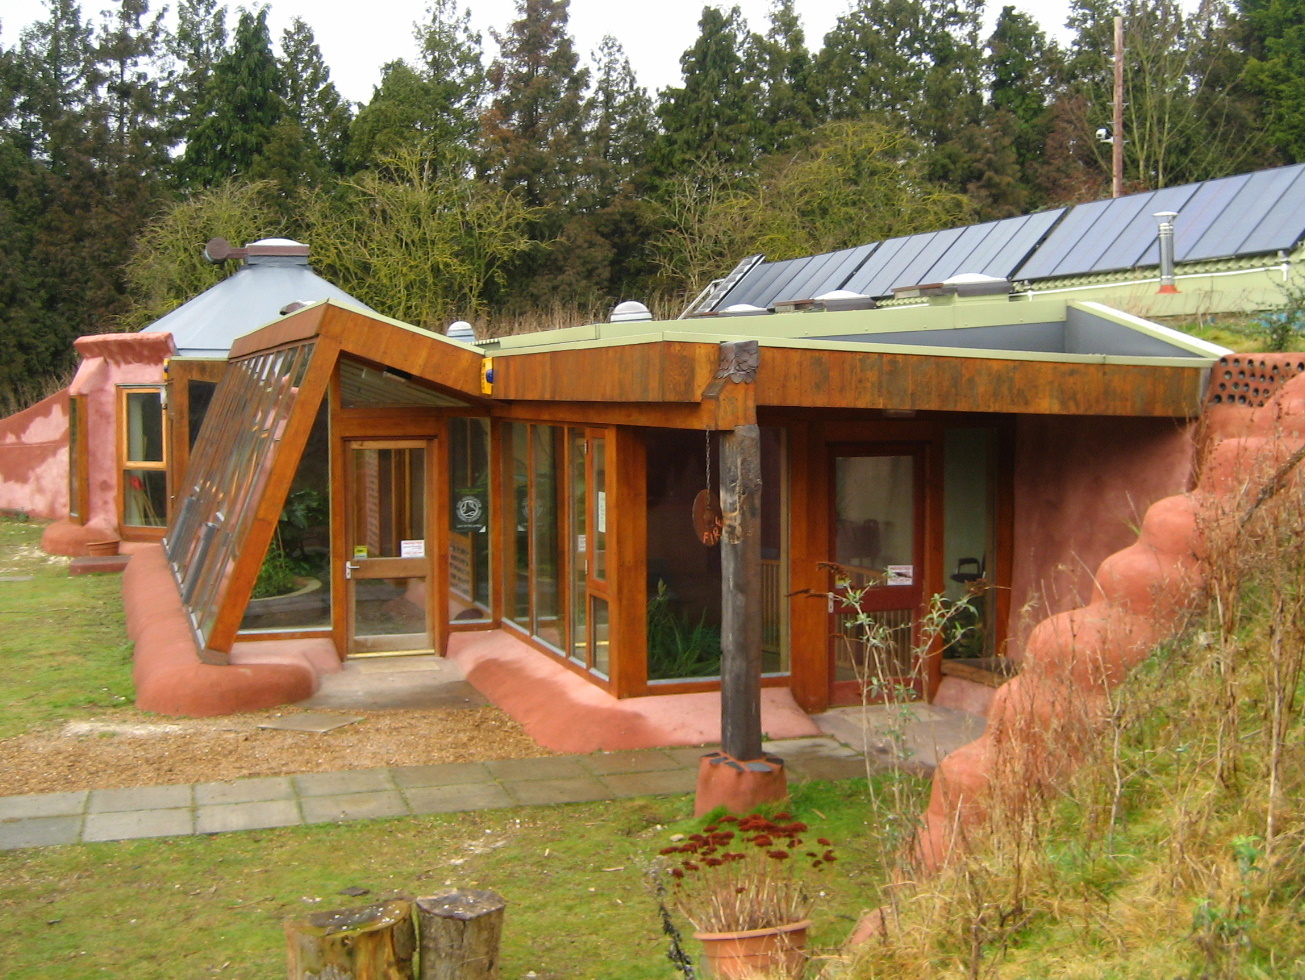
\includegraphics[width=.9\linewidth]{./pictures/earthship-brighton.jpg}
\caption{\label{fig:orgeb47be1}Earthship Brighton, UK}
\end{figure}

\section{ชุมชนที่ยั่งยืน}
\label{sec:orgacd63d2}
คราวนี้มาลองพิจารณาความยั่งยืนในระดับที่ใหญ่ขึ้นบ้าง ในชุมชนที่ชื่อว่า
Kaikoura ในประเทศนิวซีแลนด์
นับเป็นหนึ่งในชุมชนที่ได้ชื่อว่ามีความยั่งยืน อันเนื่องมาจาก

\begin{itemize}
\item มีระบบนิเวศที่อุดมสมบูรณ์และมีความหลากหลายทำหน้าที่เป็นแหล่งผลิตทรัพยากรให้มนุษย์

\item มีรากฐานทางสังคมที่ส่งเสริมคุณภาพชีวิตของประชากรในชุมชน
ให้ความเคารพกับความแตกต่างทางวัฒนธรรม ให้ความสำคัญกับความเท่าเทียมกัน
และเล็งเห็นถึงความต้องการของประชากรในรุ่นต่อๆไป

\item มีเศรษฐกิจที่มีความหลากหลายเพียงพอที่จะรับกับความเปลี่ยนแปลง
สร้างความมั่นคงให้กับประชากรได้ในระยะยาว รวมทั้ง
\end{itemize}

\section{กรณีศึกษา: ศักยภาพของเชื้อเพลิงชีวภาพต่อการพัฒนาที่ยั่งยืนในอนุภูมิภาคลุ่มแม่น้ำโขง}
\label{sec:orgb56d80c}
\subsubsection{ข้อมูลเบื้องต้น}
\label{sec:org2f43469}
อนุภูมิภาคลุ่มแม่น้ำโขง (Greater Mekong Subregion: GMS)
ประกอบไปด้วยประเทศและมณฑลที่อยู่ในบริเวณที่ราบลุ่มแม่น้ำโขงอันประกอบไปด้วยประเทศกัมพูชา
ลาว เมียนมาร์ เวียดนาม มณฑลยูนนาน และมณฑลกว่างซีในประเทศจีน
มีประชากรรวมกว่า 325 ล้านคน (2008)
และมีทรัพยาการธรรมชาติมากมายไม่ว่าจะเป็นไม้ แร่ธาติ ถ่านหิน ปิโตรเลียม
รวมถึงแม่น้ำย่อยอีกหลายสาย

\subsubsection{ความร่วมมือทางเศรษฐกิจในอนุภูมิภาคลุ่มแม่น้ำโขง}
\label{sec:org4e65bd5}
เป็นแผนความร่วมมือที่เน้นถึงการปฏิรูปทางเศรษฐกิจว่าด้วยเรื่องของการเชื่อมโยงคมนาคม
โทรคมนาคม และการค้าขายข้ามชายแดน อันอาจจะส่งผลกระทบถึงทรัพยากรธรรมชาติ
ไม่ว่าจะเป็นเรื่องของการสูญเสียทางระบบนิเวศน์ พืชพรรณ
และสัตว์ป่าต่างๆด้วย

\subsubsection{ศักยภาพของการใช้เชื้อเพลิงชีวภาพเพื่อการพัฒนาที่ยังยืนใน GMS}
\label{sec:org7d17d4c}
การใช้เชื้อเพลิงที่มีแหล่งที่มาจากใน GMS
เองย่อมส่งผลดีต่อความมั่นคงทางด้านพลังงานของอนุภูมิภาค
ลดการพึ่งพาการนำเข้าปิโตรเลียม
นอกจากนี้ยังเป็นการสร้างงานและขยายตลาดของผลิตผลทางการเกษตร
ซึ่งเป็นการช่วยกระตุ้นเศรษฐกิจภาคการเกษตรและกระจายรายได้สู่ชนบท
และท้ายที่สุดแล้วเชื้อเพลิงชีวภาพเป็นเชื้อเพลิงที่ปล่อยคาร์บอนสุทธิเป็นศูนย์หรือติดลบ
ซึ่งส่งผลดีต่อการป้องกันภาวะโลกร้อนและการเปลี่ยนสภาพชองภูมิอากาศ

ความซับซ้อนของการวิเคราะห์โครงการนี้มีจากการที่จะต้องพัฒนามีการพัฒนาปรับปรุงขนาดใหญ่ครอบคลุมภูมิภาค
ต้องมีการส่งเสริมให้ประชากรหันมาใช้เชื้อเพลิงชนิดใหม่
นอกจากนี้ยังมีผู้เกี่ยวข้องที่ได้รับผลประโยชน์และผลกระทบหลายฝ่าย
จึงจำเป็นจะต้องมีการวางแผนอย่างรัดกุม
วิเคราะห์ผลลัพธ์ที่จะเกิดขึ้นจากทุกด้าน

\subsubsection{ประเด็นที่พึงคำนึงถึงในหนทางสู่เชื้อเพลิงชีวภาพ}
\label{sec:org5cef7d1}

\begin{enumerate}
\item การเปลี่ยนแปลงของภูมิอากาศและสิ่งแวดล้อม

\item ผลกระทบต่อคนยากจนและคนในชนบท

\item เทคโนโลยีและวัตถุดิบที่จะใช้

\item โครงสร้างพื้นฐาน

\item การบริหารและจัดการ

\item นโยบายที่เกี่ยวข้อง
\end{enumerate}

\subsubsection{การดำเนินการ}
\label{sec:orge7989ae}
จากประเด็นที่พีงคำนึง
เราสามารถนำมาวิเคราะห์เป็นกลุ่มปัญหาอย่างเช่นเรื่องของกลุ่มอุตสาหกรรมคมนาคม
ห่วงโซ่อุปทาน เทคโนโลยีที่เหมาะสม การร่างนโยบาย
การสรรหาแหล่งเงินทุนและการสร้างขีดความสามารถ
ซึ่งประเด็นเหล่านี้จะต้องนำมาอภิปรายเมื่อได้ไปตรวจเยี่ยมสถานที่จริงที่ประเทศกัมพูชา
เวียดนาม ลาว มณฑลยูนนาน และประเทศไทย
โดยได้ทำการสัมภาษณ์และรับฟังข้อเสนอแนะ
รวมถึงข้อวิพากษ์วิจารณ์จากหลายหน่วยงาน ไม่ว่าจะเป็นบริษัทพลังงานท้องถิ่น
นักลงทุน ธนาคารนานาชาติ หน่วยงานพิทักษ์สิ่งแวดล้อม องค์การเพื่อการพัฒนา
สถาบันวิจัย มหาวิทยาลัย หน่วยงานท้องถิ่นด้านอุตสาหกรรม พลังงาน ป่าไม้
สิ่งแวดล้อม เกษตรกรรม คมนาคม พาณิชย์ พัฒนาท้องถิ่น และนโยบาย

\subsubsection{มิติด้านนโยบาย}
\label{sec:org799ec75}

\begin{itemize}
\item แต่ละประเทศควรมีนโยบายเกี่ยวกับเชื้อเพลิงชีวภาพที่สอดคล้องกัน
และมีแผนพัฒนาร่วมกันในระยะยาว
ทั้งนี้เพื่อให้มีมาตรฐานในการผลิตและใช้เชื้อเพลิงเดียวกัน
มีการส่งเสริมการลงทุน การให้แรงจูงใจทางภาษี การกำหนดการใช้ที่ดิน
การกำหนดมาตรฐานของเชื้อเพลิงชีวภาพ การกำหนดคุณลักษณะของยานพาหนะ
โลจิสติกส์

\item การร่างนโยบายระดับชาติโดยได้รับความร่วมมือจากทุกกระทรวงที่เกี่ยวข้อง

\item มีโครงสร้างแรงจูงใจที่จะช่วยเร่งสร้างห่วงโซ่อุปทานสำหรับธุรกิจเชื้อเพลิงชีวภาพรุ่นแรกๆ

\item กำหนดมาตรฐานภาคบังคับเพื่อรับประกันคุณภาพและประสิทธิภาพด้านสิ่งแวดล้อม
และเพื่อสร้างความมั่นใจแก่ผู้บริโภค

\item การกำหนดมาตรฐานร่วมในภูมิภาคเดียวกัน

\item การกำหนดนโยบายอื่นๆที่เกี่ยวข้องเพื่อช่วยในการลดคาร์บอน ลดความยากจน
รักษาความหลากทางชีวภาพ และเพิ่มความมั่นคงทางพลังงานให้แก่ภูมิภาค
\end{itemize}

\subsubsection{มิติด้านการกำกับดูแลและการจัดการ}
\label{sec:orge67d428}

\begin{itemize}
\item การกำกับดูแลการปลูกพืชเชื้อเพลิงชีวภาพในที่สัมปทาน
เพื่อลดปัญหาจากการแสวงหาประโยชน์ในทางที่ผิดเช่นการถางป่าหรือทำไร่เลื่อนลอย
มีการตรวจสอบผู้ได้รับสัมปทานและติดตามผล มีการจัดแบ่งโซนการเพาะปลูก

\item มีการจัดการห่วงโซ่อุปทานดีเพื่อหลีกเลี่ยงปัญหาจากการกระจายตัวของแหล่งผลิต
\end{itemize}

\subsubsection{มิติด้านโครงสร้างพื้นฐาน}
\label{sec:org7cbbb51}

\begin{itemize}
\item ต้องมีการลงทุนอย่างมหาศาลในโครงสร้างพื้นฐานสำหรับการวิจัยและพัฒนา
การกลั่น การกระจายสินค้า
และการกักเก็บเชื้อเพลิงชีวภาพสำหรับการใช้ในภาคคมนาคม

\item การลงทุนจากฝ่ายเอกชนและจากต่างชาติเพื่อส่งเสริมทรัพยากรบางส่วนที่อาจจะมีอยู่จำกัดในท้องถิ่น
\end{itemize}

\subsubsection{มิติด้านการใช้เทคโนโลยีและวัตถุดิบที่เหมาะสม}
\label{sec:org1849678}

\begin{itemize}
\item ต้องเลือกวัตถุดิบที่ไม่ต้องใช้เป็นอาหาร
ไม่ต้องใช้พื้นที่เพาะปลูกที่ใช้ในอุตสาหกรรมการผลิตอาหาร ยกตัวอย่างเช่น
ไม่ไปแย่งพื้นที่ในการปลูกข้าว พืชผัก
หรือแม้แต่พืชที่ใช้เป็นอาหารสัตว์ที่นำมาเป็นอาหาร
และต้องเป็นพืชที่ให้อัตราผลผลิต (แป้ง น้ำมัน น้ำตาลหรืออื่นๆ)

\item พิจารณาการสร้างรายได้เพิ่มเติมจากพืชวัตถุดิบ เช่น นำมาทำเป็นยาสมุนไพร
อาหารสัตว์ ปุ๋ยหมัก หรืออาหารเสริม

\item ใช้เทคโนโลยีการผลิตที่เหมาะสมกับท้องถิ่น
\end{itemize}

\subsubsection{มิติด้านผลกระทบต่อความเป็นอยู่ของคนยากจนและคนในชนบท}
\label{sec:org80e9b9e}

\begin{itemize}
\item สร้างรายได้เพิ่มเติมให้กับประชาชนทั้งในระดับครัวเรือนและชุมชนจากการผลิตเชื้อเพลิงชีวภาพขนาดย่อม
เช่นการปลูกพืชวัตถุดิบบนที่ดินชายขอบเป็นรายได้เพิ่ม
การสร้างงานจากการสร้างโครงสร้างพื้นฐาน หรือการจ้างงานในสวน

\item การประเมินความเสี่ยงจากผลผลิตล้นตลาดจากการที่ราคาพืชวัตถุดิบพุ่งสูงขึ้นชั่วคราว
ทำให้เกษตรกรหันมาปลูกมากเกินไปจนทำให้ราคาตก
ซึ่งตัวอย่างนี้เราเห็นได้เป็นประจำไม่ว่าจะเป็นกรณีของข้าว ยางพารา
มะนาว

\item การทุจริตสัมปทาน บุกรุกพื้นที่ป่า นายทุนกว้านซื้อที่ดิน
การสูญเสียรายได้ การพลัดถิ่นฐานอันมีผลมาจากการพัฒนา
การสร้างโครงสร้างพื้นฐานอาจมีผลกระทบถึงความสามารถในการเข้าถึงถนน น้ำ
และไฟฟ้า
\end{itemize}

\subsubsection{มิติด้านการเปลี่ยนแปลงสภาพภูมิอากาศและสิ่งแวดล้อม}
\label{sec:orga5f5609}

\begin{itemize}
\item การปลูกป่าทดแทนบนที่ดินชายขอบในสวนขนาดใหญ่แม้จะเป็นพื้นที่เพียงเล็กน้อย
ฟื้นฟูหน้าที่ทางระบบนิเวศบางส่วนเช่นการป้องกันการกัดเซาะหน้าดิบ

\item ในสวนที่มีการจัดการที่ไม่ดี อาจมีปัญหาของการตัดไม้ทำลายป่า
การสูญเสียความหลากหลายทางชีวภาพ การแก่งแย่งทรัพยากรธรรมชาติ
ผลกระทบกับคุณภาพของดิน

\item การให้สัมปทานอาจก่อให้เกิดการตัดไม้ทำลายป่า
ซึ่งจะหักล้างกับผลประโยชน์การลดแก็สเรือนกระจกที่ได้จากการเปลี่ยนมาใช้พลังงานจากเชื้อเพลิงชีวภาพ
\end{itemize}

\subsubsection{สรุป}
\label{sec:orgb48b1e9}
เชื้อเพลิงชีวภาพเป็นหนทางหนึ่งอันจะพาไปสู่การพัฒนาที่ยั่งยืนได้
ไม่ว่าจะเป็นเรื่องของการพัฒนาแหล่งพลังงานในประเทศ สร้างงานและความมั่นคง
ขยายตลาดผลผลิตทางการเกษตร และการลดการปล่อยคาร์บอนสู่บรรยากาศ อย่างไรก็ดี
ในหนทางการพัฒนานี้ หากไม่มีการจัดการและวางแผนที่ดี
อาจจะเกิดผลเสียขึ้นได้หลายประการตามที่ได้กล่าวมา
โดยเฉพาะอย่างยิ่งในประเทศกำลังพัฒนาซึ่งอาจจะยังมีปัญหาเรื่องของการบังคับใช้กฎ
ระเบียบ และมาตรฐานต่างๆ

\section{กรณีศึกษา 2: การพัฒนาและใช้น้ำมันไบโอดีเซลในมหาวิทยาลัยธรรมศาสตร์}
\label{sec:orgb73d455}
ในกรณีศึกษาที่แล้ว โครงการมีขนาดใหญ่ ครอบคลุมพื้นที่ขนาดอนุภูมิภาค
คราวนี้เรามาลองทำความเข้าใจโครงการ(สมมติ)ที่มีขนาดเล็กลงในมหาวิทยาลัยธรรมศาสตร์(ซึ่งใกล้ตัวเรามากขึ้น)
ลองพิจารณาความยั่งยืนของนโยบายพัฒนาและบังคับใช้ไบโอดีเซลในมหาวิทยาลัยธรรมศาสตร์
ในที่นี้ประเด็นสำคัญที่เราจะต้องพิจารณาก็คือเรื่องของการผลิตไบโอดีเซลในพื้นที่มหาวิทยาลัยและเรื่องของผลกระทบต่อระบบต่างๆภายในมหาวิทยาลัย
ซึ่งเราจะสามารถแยกพิจารณาเป็น 3 หัวข้อได้ดังนี้

\begin{enumerate}
\item ด้านเศรษฐศาสตร์

\begin{itemize}
\item ต้นทุนพลังงานที่เพิ่มขึ้น/ลดลงของมหาวิทยาลัย

\item ต้นทุนคมนาคมขนส่งของนักศึกษาและบุคลากร

\item ขยายตลาดผลผลิตทางการเกษตร

\item โอกาสในการลงทุน/บั่นทอนโอกาสของเทคโนโลยีอื่น
\end{itemize}

\item ด้านสิ่งแวดล้อม

\begin{itemize}
\item การปล่อยมลพิษ

\item ของเหลือและมลภาวะจากการผลิต

\item ความหลากหลายทางชีวภาพ

\item การตัดไม้ทำลายป่า
\end{itemize}

\item ด้านสังคม

\begin{itemize}
\item ความมั่นคงทางพลังงาน

\item การสร้างงานหรือการสูญเสียงานในมหาวิทยาลัย

\item การจราจรติดขัด

\item ภาพลักษณ์ความเป็นสีเขียว

\item การแข่งขันกับการปลูกพืชเป็นอาหารในชุมชนรอบๆ

\item โอกาสในการศึกษาระบบ
\end{itemize}
\end{enumerate}

\section{ตัวบ่งชี้ความยั่งยืน}
\label{sec:org67b4812}
แม้ว่าเราจะมีความเข้าใจว่าความยั่งยืนหมายถึงอะไร
แต่ก็ยังเป็นความเข้าใจในเชิงนามธรรม
ซึ่งหากเราต้องการประเมินความยั่งยืนของโครงการหนึ่งๆนั้น
การจะใช้เกณฑ์ที่เป็นนามธรรมย่อมจะทำได้ยากหากเราขาดเกณฑ์ที่มีความชัดเจนเพียงพอ
จำเป็นที่เราจะต้องมีเกณฑ์ที่เป็นรูปธรรม เป็นตัวเลข
มีวิธีวัดที่ชัดเจนเพื่อที่จะสามารถประเมินความยั่งยืนได้อย่างมีประสิทธิภาพและคงเส้นคงวา

ดังนั้น เราจะนำ\textbf{ตัวบ่งชี้}มาใช้ในการวัดความยั่งยืน
ตัวบ่งชี้มักจะเป็นค่าหรือจำนวนที่ใช้ในการวัดระดับหรือสถานะของสิ่งสิ่งหนึ่ง

ยกตัวอย่างเช่น หากเราจะหาตัวบ่งชี้ที่จะบอกสถานะความเปรี้ยวของมะนาว
บอกว่าเปรี้ยวมาก เปรี่ยวจี๊ด เปรี้ยวนิดหน่อยก็อาจจะไม่ชัดเจน
ยิ่งไปกว่านั้น เปรี้ยวมากของแต่ละคนก็ไม่เท่ากัน
ดังนั้นตัวบ่งชี้ด้วยคำพูดจะไม่เหมาะสม
เพราะไม่สามารถวัดได้สม่ำเสมอและไม่มีความชัดเจน ในกรณีนี้ เราสามารถเอาค่า
pH ของน้ำมะนาวมาเป็นตัวบ่งชี้ เนื่องจากมีวิธีการวัดที่ชัดเจนและสม่ำเสมอ

หรือหากต้องการหาตัวบ่งชี้ความสดของมะนาว
การจะใช้สีเปลือกหรือวัดความแน่นของเนื้อด้วยการบีบก็จะได้ค่าที่ไม่ชัดเจน
ดังนั้นเราสามารถใช้จำนวนวันนับจากวันเก็บเกี่ยวมาใช้เป็นตัวบ่งชี้ได้
เป็นต้น

แล้วถ้าจะหาตัวบ่งชี้ความยั่งยืนของโครงการ ชุมชน หรือประเทศ
จะต้องใช้ตัวบ่งชี้ทางสิ่งแวดล้อม เศรษฐกิจและสังคมตัวใดบ้าง

\subsubsection{คุณสมบัติของตัวบ่งชี้ที่ดี}
\label{sec:org07a9d25}

\begin{itemize}
\item มีความถูกต้องเหมาะสม

\item มีความเกี่ยวข้องกับผู้มีส่วนได้ส่วนเสีย

\item ต้นทุนการเก็บข้อมูลไม่สูงจนเกินไป

\item มีความน่าเชื่อถือ

\item เข้าใจและตีความได้ง่าย

\item มีมาตรฐานเพื่อใช้เปรียบเทียบ

\item สามารถแสดงแนวโน้มเมื่อเวลาผ่านไปได้

\item ตั้งกรอบทั้งด้านเวลาและบริเวณอย่างเหมาะสม
\end{itemize}

\section{กระบวนการประเมินความยั่งยืน}
\label{sec:orge2a0136}
การประเมินความยั่งยืนคือการนำเอาตัวบ่งชี้ที่วัดได้มาวิเคราะห์และแปรผลออกมา โดยจริงๆแล้วผลจะไม่ได้ออกมาเป็นแบบผ่านหรือไม่ผ่าน แต่จะออกมาเป็นค่าตัวบ่งชี้เพื่อช่วยให้ผู้ประเมินมองเห็นในภาพรวมว่าโครงการมีผลกระทบด้านบวกและด้านลบทางเศรษฐกิจ สังคม และสิ่งแวดล้อมอย่างไรบ้าง และสามารถนำไปเปรียบเทียบกับโครงการทางเลือกอื่นๆได้ โดยกระบวนการประเมินนั้นก็สามารถแยกย่อยออกมา

\chapter{พลังงานในประเทศไทย}
\label{sec:org4fd983b}

\backmatter

\hypertarget{citeproc_bib_item_1}{[1] J. P. Heremans \textit{et al.}, “Enhancement of thermoelectric efficiency in pbte by distortion of the electronic density of states,” \textit{Science}, vol. 321, no. 5888, pp. 554–557, 2008.}

\hypertarget{citeproc_bib_item_2}{[2] Y. Pei, A. LaLonde, S. Iwanaga, and G. J. Snyder, “High thermoelectric figure of merit in heavy hole dominated pbte,” \textit{Energy \& environmental science}, vol. 4, no. 6, pp. 2085–2089, 2011.}

\hypertarget{citeproc_bib_item_3}{[3] K. Biswas \textit{et al.}, “High-performance bulk thermoelectrics with all-scale hierarchical architectures,” \textit{Nature}, vol. 489, no. 7416, p. 414, 2012.}

\hypertarget{citeproc_bib_item_4}{[4] S. Sukkasi, “Biofuels,” \textit{Energy sources and conversion}, 2015.}

\hypertarget{citeproc_bib_item_5}{[5] I. Baird and N. Quastel, “Rescaling and reordering nature–society relations: The nam theun 2 hydropower dam and laos–thailand electricity networks,” \textit{Annals of the association of american geographers}, 2015, doi: \href{https://doi.org/10.1080/00045608.2015.1064511}{10.1080/00045608.2015.1064511}.}\bigskip
\end{document}